
%% bare_jrnl.tex
%% V1.4b
%% 2015/08/26
%% by Michael Shell
%% see http://www.michaelshell.org/
%% for current contact information.
%%
%% This is a skeleton file demonstrating the use of IEEEtran.cls
%% (requires IEEEtran.cls version 1.8b or later) with an IEEE
%% journal paper.
%%
%% Support sites:
%% http://www.michaelshell.org/tex/ieeetran/
%% http://www.ctan.org/pkg/ieeetran
%% and
%% http://www.ieee.org/

%%*************************************************************************
%% Legal Notice:
%% This code is offered as-is without any warranty either expressed or
%% implied; without even the implied warranty of MERCHANTABILITY or
%% FITNESS FOR A PARTICULAR PURPOSE! 
%% User assumes all risk.
%% In no event shall the IEEE or any contributor to this code be liable for
%% any damages or losses, including, but not limited to, incidental,
%% consequential, or any other damages, resulting from the use or misuse
%% of any information contained here.
%%
%% All comments are the opinions of their respective authors and are not
%% necessarily endorsed by the IEEE.
%%
%% This work is distributed under the LaTeX Project Public License (LPPL)
%% ( http://www.latex-project.org/ ) version 1.3, and may be freely used,
%% distributed and modified. A copy of the LPPL, version 1.3, is included
%% in the base LaTeX documentation of all distributions of LaTeX released
%% 2003/12/01 or later.
%% Retain all contribution notices and credits.
%% ** Modified files should be clearly indicated as such, including  **
%% ** renaming them and changing author support contact information. **
%%*************************************************************************


% *** Authors should verify (and, if needed, correct) their LaTeX system  ***
% *** with the testflow diagnostic prior to trusting their LaTeX platform ***
% *** with production work. The IEEE's font choices and paper sizes can   ***
% *** trigger bugs that do not appear when using other class files.       ***                          ***
% The testflow support page is at:
% http://www.michaelshell.org/tex/testflow/



\documentclass[journal]{IEEEtran}
%
% If IEEEtran.cls has not been installed into the LaTeX system files,
% manually specify the path to it like:
% \documentclass[journal]{../sty/IEEEtran}





% Some very useful LaTeX packages include:
% (uncomment the ones you want to load)

% added package
% \usepackage{graphicx}%插入图片
\usepackage{amssymb}%数学符号
\usepackage{amsthm}%数学定理
\usepackage{amsmath}%数学公式、矩阵、积分求和等
\usepackage{lineno}%显示行号
\usepackage{txfonts} %默认字体times new roman
\usepackage{enumitem}%项目编号
\usepackage{multirow} %多行合并
\usepackage{caption} %改变图表标题
\usepackage{txfonts} %默认字体times new roman
\usepackage{array} %\调用公式宏包的命令应放在调用定理宏包命令之前,也能控制表格
\usepackage{booktabs} %调整表格线与上下内容的间隔
\usepackage{longtable}%调用跨页表格
\usepackage{bm}%数学字体加粗
\usepackage{setspace} %调整一段文字的行间距
\usepackage[comma, numbers,square]{natbib} %参考文献管理包
\usepackage{subfigure}
%% The amssymb package provides various useful mathematical symbols
\usepackage{amssymb}
% %% The amsthm package provides extended theorem environments
\usepackage{amsthm}



% *** MISC UTILITY PACKAGES ***
%
%\usepackage{ifpdf}
% Heiko Oberdiek's ifpdf.sty is very useful if you need conditional
% compilation based on whether the output is pdf or dvi.
% usage:
% \ifpdf
%   % pdf code
% \else
%   % dvi code
% \fi
% The latest version of ifpdf.sty can be obtained from:
% http://www.ctan.org/pkg/ifpdf
% Also, note that IEEEtran.cls V1.7 and later provides a builtin
% \ifCLASSINFOpdf conditional that works the same way.
% When switching from latex to pdflatex and vice-versa, the compiler may
% have to be run twice to clear warning/error messages.






% *** CITATION PACKAGES ***
%
% \usepackage{cite}
% cite.sty was written by Donald Arseneau
% V1.6 and later of IEEEtran pre-defines the format of the cite.sty package
% \cite{} output to follow that of the IEEE. Loading the cite package will
% result in citation numbers being automatically sorted and properly
% "compressed/ranged". e.g., [1], [9], [2], [7], [5], [6] without using
% cite.sty will become [1], [2], [5]--[7], [9] using cite.sty. cite.sty's
% \cite will automatically add leading space, if needed. Use cite.sty's
% noadjust option (cite.sty V3.8 and later) if you want to turn this off
% such as if a citation ever needs to be enclosed in parenthesis.
% cite.sty is already installed on most LaTeX systems. Be sure and use
% version 5.0 (2009-03-20) and later if using hyperref.sty.
% The latest version can be obtained at:
% http://www.ctan.org/pkg/cite
% The documentation is contained in the cite.sty file itself.






% *** GRAPHICS RELATED PACKAGES ***
%
\ifCLASSINFOpdf
   \usepackage[pdftex]{graphicx}
  % declare the path(s) where your graphic files are
  % \graphicspath{{../pdf/}{../jpeg/}}
  % and their extensions so you won't have to specify these with
  % every instance of \includegraphics
  % \DeclareGraphicsExtensions{.pdf,.jpeg,.png}
\else
  % or other class option (dvipsone, dvipdf, if not using dvips). graphicx
  % will default to the driver specified in the system graphics.cfg if no
  % driver is specified.
   \usepackage[dvips]{graphicx}
  % declare the path(s) where your graphic files are
  % \graphicspath{{../eps/}}
  % and their extensions so you won't have to specify these with
  % every instance of \includegraphics
  % \DeclareGraphicsExtensions{.eps}
\fi
% graphicx was written by David Carlisle and Sebastian Rahtz. It is
% required if you want graphics, photos, etc. graphicx.sty is already
% installed on most LaTeX systems. The latest version and documentation
% can be obtained at: 
% http://www.ctan.org/pkg/graphicx
% Another good source of documentation is "Using Imported Graphics in
% LaTeX2e" by Keith Reckdahl which can be found at:
% http://www.ctan.org/pkg/epslatex
%
% latex, and pdflatex in dvi mode, support graphics in encapsulated
% postscript (.eps) format. pdflatex in pdf mode supports graphics
% in .pdf, .jpeg, .png and .mps (metapost) formats. Users should ensure
% that all non-photo figures use a vector format (.eps, .pdf, .mps) and
% not a bitmapped formats (.jpeg, .png). The IEEE frowns on bitmapped formats
% which can result in "jaggedy"/blurry rendering of lines and letters as
% well as large increases in file sizes.
%
% You can find documentation about the pdfTeX application at:
% http://www.tug.org/applications/pdftex





% *** MATH PACKAGES ***
%
%\usepackage{amsmath}
% A popular package from the American Mathematical Society that provides
% many useful and powerful commands for dealing with mathematics.
%
% Note that the amsmath package sets \interdisplaylinepenalty to 10000
% thus preventing page breaks from occurring within multiline equations. Use:
%\interdisplaylinepenalty=2500
% after loading amsmath to restore such page breaks as IEEEtran.cls normally
% does. amsmath.sty is already installed on most LaTeX systems. The latest
% version and documentation can be obtained at:
% http://www.ctan.org/pkg/amsmath





% *** SPECIALIZED LIST PACKAGES ***
%
%\usepackage{algorithmic}
% algorithmic.sty was written by Peter Williams and Rogerio Brito.
% This package provides an algorithmic environment fo describing algorithms.
% You can use the algorithmic environment in-text or within a figure
% environment to provide for a floating algorithm. Do NOT use the algorithm
% floating environment provided by algorithm.sty (by the same authors) or
% algorithm2e.sty (by Christophe Fiorio) as the IEEE does not use dedicated
% algorithm float types and packages that provide these will not provide
% correct IEEE style captions. The latest version and documentation of
% algorithmic.sty can be obtained at:
% http://www.ctan.org/pkg/algorithms
% Also of interest may be the (relatively newer and more customizable)
% algorithmicx.sty package by Szasz Janos:
% http://www.ctan.org/pkg/algorithmicx




% *** ALIGNMENT PACKAGES ***
%
%\usepackage{array}
% Frank Mittelbach's and David Carlisle's array.sty patches and improves
% the standard LaTeX2e array and tabular environments to provide better
% appearance and additional user controls. As the default LaTeX2e table
% generation code is lacking to the point of almost being broken with
% respect to the quality of the end results, all users are strongly
% advised to use an enhanced (at the very least that provided by array.sty)
% set of table tools. array.sty is already installed on most systems. The
% latest version and documentation can be obtained at:
% http://www.ctan.org/pkg/array


% IEEEtran contains the IEEEeqnarray family of commands that can be used to
% generate multiline equations as well as matrices, tables, etc., of high
% quality.




% *** SUBFIGURE PACKAGES ***
%\ifCLASSOPTIONcompsoc
%  \usepackage[caption=false,font=normalsize,labelfont=sf,textfont=sf]{subfig}
%\else
%  \usepackage[caption=false,font=footnotesize]{subfig}
%\fi
% subfig.sty, written by Steven Douglas Cochran, is the modern replacement
% for subfigure.sty, the latter of which is no longer maintained and is
% incompatible with some LaTeX packages including fixltx2e. However,
% subfig.sty requires and automatically loads Axel Sommerfeldt's caption.sty
% which will override IEEEtran.cls' handling of captions and this will result
% in non-IEEE style figure/table captions. To prevent this problem, be sure
% and invoke subfig.sty's "caption=false" package option (available since
% subfig.sty version 1.3, 2005/06/28) as this is will preserve IEEEtran.cls
% handling of captions.
% Note that the Computer Society format requires a larger sans serif font
% than the serif footnote size font used in traditional IEEE formatting
% and thus the need to invoke different subfig.sty package options depending
% on whether compsoc mode has been enabled.
%
% The latest version and documentation of subfig.sty can be obtained at:
% http://www.ctan.org/pkg/subfig




% *** FLOAT PACKAGES ***
%
%\usepackage{fixltx2e}
% fixltx2e, the successor to the earlier fix2col.sty, was written by
% Frank Mittelbach and David Carlisle. This package corrects a few problems
% in the LaTeX2e kernel, the most notable of which is that in current
% LaTeX2e releases, the ordering of single and double column floats is not
% guaranteed to be preserved. Thus, an unpatched LaTeX2e can allow a
% single column figure to be placed prior to an earlier double column
% figure.
% Be aware that LaTeX2e kernels dated 2015 and later have fixltx2e.sty's
% corrections already built into the system in which case a warning will
% be issued if an attempt is made to load fixltx2e.sty as it is no longer
% needed.
% The latest version and documentation can be found at:
% http://www.ctan.org/pkg/fixltx2e


%\usepackage{stfloats}
% stfloats.sty was written by Sigitas Tolusis. This package gives LaTeX2e
% the ability to do double column floats at the bottom of the page as well
% as the top. (e.g., "\begin{figure*}[!b]" is not normally possible in
% LaTeX2e). It also provides a command:
%\fnbelowfloat
% to enable the placement of footnotes below bottom floats (the standard
% LaTeX2e kernel puts them above bottom floats). This is an invasive package
% which rewrites many portions of the LaTeX2e float routines. It may not work
% with other packages that modify the LaTeX2e float routines. The latest
% version and documentation can be obtained at:
% http://www.ctan.org/pkg/stfloats
% Do not use the stfloats baselinefloat ability as the IEEE does not allow
% \baselineskip to stretch. Authors submitting work to the IEEE should note
% that the IEEE rarely uses double column equations and that authors should try
% to avoid such use. Do not be tempted to use the cuted.sty or midfloat.sty
% packages (also by Sigitas Tolusis) as the IEEE does not format its papers in
% such ways.
% Do not attempt to use stfloats with fixltx2e as they are incompatible.
% Instead, use Morten Hogholm'a dblfloatfix which combines the features
% of both fixltx2e and stfloats:
%
% \usepackage{dblfloatfix}
% The latest version can be found at:
% http://www.ctan.org/pkg/dblfloatfix




%\ifCLASSOPTIONcaptionsoff
%  \usepackage[nomarkers]{endfloat}
% \let\MYoriglatexcaption\caption
% \renewcommand{\caption}[2][\relax]{\MYoriglatexcaption[#2]{#2}}
%\fi
% endfloat.sty was written by James Darrell McCauley, Jeff Goldberg and 
% Axel Sommerfeldt. This package may be useful when used in conjunction with 
% IEEEtran.cls'  captionsoff option. Some IEEE journals/societies require that
% submissions have lists of figures/tables at the end of the paper and that
% figures/tables without any captions are placed on a page by themselves at
% the end of the document. If needed, the draftcls IEEEtran class option or
% \CLASSINPUTbaselinestretch interface can be used to increase the line
% spacing as well. Be sure and use the nomarkers option of endfloat to
% prevent endfloat from "marking" where the figures would have been placed
% in the text. The two hack lines of code above are a slight modification of
% that suggested by in the endfloat docs (section 8.4.1) to ensure that
% the full captions always appear in the list of figures/tables - even if
% the user used the short optional argument of \caption[]{}.
% IEEE papers do not typically make use of \caption[]'s optional argument,
% so this should not be an issue. A similar trick can be used to disable
% captions of packages such as subfig.sty that lack options to turn off
% the subcaptions:
% For subfig.sty:
% \let\MYorigsubfloat\subfloat
% \renewcommand{\subfloat}[2][\relax]{\MYorigsubfloat[]{#2}}
% However, the above trick will not work if both optional arguments of
% the \subfloat command are used. Furthermore, there needs to be a
% description of each subfigure *somewhere* and endfloat does not add
% subfigure captions to its list of figures. Thus, the best approach is to
% avoid the use of subfigure captions (many IEEE journals avoid them anyway)
% and instead reference/explain all the subfigures within the main caption.
% The latest version of endfloat.sty and its documentation can obtained at:
% http://www.ctan.org/pkg/endfloat
%
% The IEEEtran \ifCLASSOPTIONcaptionsoff conditional can also be used
% later in the document, say, to conditionally put the References on a 
% page by themselves.




% *** PDF, URL AND HYPERLINK PACKAGES ***
%
%\usepackage{url}
% url.sty was written by Donald Arseneau. It provides better support for
% handling and breaking URLs. url.sty is already installed on most LaTeX
% systems. The latest version and documentation can be obtained at:
% http://www.ctan.org/pkg/url
% Basically, \url{my_url_here}.




% *** Do not adjust lengths that control margins, column widths, etc. ***
% *** Do not use packages that alter fonts (such as pslatex).         ***
% There should be no need to do such things with IEEEtran.cls V1.6 and later.
% (Unless specifically asked to do so by the journal or conference you plan
% to submit to, of course. )


% correct bad hyphenation here
\hyphenation{op-tical net-works semi-conduc-tor}


\begin{document}
%
% paper title
% Titles are generally capitalized except for words such as a, an, and, as,
% at, but, by, for, in, nor, of, on, or, the, to and up, which are usually
% not capitalized unless they are the first or last word of the title.
% Linebreaks \\ can be used within to get better formatting as desired.
% Do not put math or special symbols in the title.
\title{Cooperative Adaptive Cruise Platoon Controller Design Considering Switching Control and Stability}
%
%
% author names and IEEE memberships
% note positions of commas and nonbreaking spaces ( ~ ) LaTeX will not break
% a structure at a ~ so this keeps an author's name from being broken across
% two lines.
% use \thanks{} to gain access to the first footnote area
% a separate \thanks must be used for each paragraph as LaTeX2e's \thanks
% was not built to handle multiple paragraphs
%

\author{Hao~Wang,
  Tiancheng~Ruan,
  Zewen~Zuo,
  Yuxuan~Hou,
  Rui~Jiang,
  \thanks{H. Wang, T. Ruan, Z. Zuo and Y. Hou are with the
    School of Transportation, Southeast University, Nanjing 211189, P.R. China;
    Jiangsu Key Laboratory of Urban ITS, Southeast University, Nanjing, 210096, P.R. China;
    Jiangsu Province Collaborative Innovation Center of Modern Urban Traffic Technologies, Southeast University, Nanjing, 210096, P.R. China(e-mail: haowang@seu.edu.cn;ruantiancheng@seu.edu.cn; 220203312@seu.edu.cn;NOTEVENWRONG@outlook.com).}% <-this % stops a space
  \thanks{J. Rui is with Key Laboratory of Transport Industry of Big Data Application Technologies for Comprehensive Transport, Ministry of Transport, Beijing Jiaotong University, Beijing, 100044,  China(e-mail: jiangrui@bjtu.edu.cn).}% <-this % stops a space
  % await for specific detail
  \thanks{Manuscript received September 21, 2022.(Corresponding author: Hao Wang.)}}

% note the % following the last \IEEEmembership and also \thanks - 
% these prevent an unwanted space from occurring between the last author name
% and the end of the author line. i.e., if you had this:
% 
% \author{....lastname \thanks{...} \thanks{...} }
%                     ^------------^------------^----Do not want these spaces!
%
% a space would be appended to the last name and could cause every name on that
% line to be shifted left slightly. This is one of those "LaTeX things". For
% instance, "\textbf{A} \textbf{B}" will typeset as "A B" not "AB". To get
% "AB" then you have to do: "\textbf{A}\textbf{B}"
% \thanks is no different in this regard, so shield the last } of each \thanks
% that ends a line with a % and do not let a space in before the next \thanks.
% Spaces after \IEEEmembership other than the last one are OK (and needed) as
% you are supposed to have spaces between the names. For what it is worth,
% this is a minor point as most people would not even notice if the said evil
% space somehow managed to creep in.



% The paper headers
% \markboth{Journal of \LaTeX\ Class Files,~Vol.~14, No.~8, August~2015}%
% {Shell \MakeLowercase{\textit{et al.}}: Bare Demo of IEEEtran.cls for IEEE Journals}
% The only time the second header will appear is for the odd numbered pages
% after the title page when using the twoside option.
% 
% *** Note that you probably will NOT want to include the author's ***
% *** name in the headers of peer review papers.                   ***
% You can use \ifCLASSOPTIONpeerreview for conditional compilation here if
% you desire.




% If you want to put a publisher's ID mark on the page you can do it like
% this:
%\IEEEpubid{0000--0000/00\$00.00~\copyright~2015 IEEE}
% Remember, if you use this you must call \IEEEpubidadjcol in the second
% column for its text to clear the IEEEpubid mark.



% use for special paper notices
%\IEEEspecialpapernotice{(Invited Paper)}




% make the title area
\maketitle

% As a general rule, do not put math, special symbols or citations
% in the abstract or keywords.
\begin{abstract}
  With the development of Cooperative Adaptive Cruise Control (CACC) technology, CACC Market Penetration Rate (MPR) is expected to increase rapidly, resulting in more CACC platoons. However, the single vehicle control mode makes it difficult to take full advantage of the gain of CACC for capacity. Moreover, the platoon control model with a fixed platoon size is also ineffective since the size of the CACC platoon is arbitrary depending on the dispersion of CACCs and Manual Vehicles (MVs). Therefore, this paper first proposed a novel switching control mode — Cooperative Adaptive Cruise Platoon Control (CACPC)—that takes the CACC platoon as the control object and is adaptive to the platoon size to utilize the CACC technology further. Secondly, a switching control method, Youla-Kučera (YK) parameterization, was adopted to construct a controller class that can stabilize the CACC platoon, thus ensuring stability while the controller switches as the platoon size changes. Then, the tuning function as the switching signal of the controller class constructed by YK parameterization is developed so that CACPC can be adaptive to different platoon sizes. Finally, numerical analyses and simulations were conducted to explore the effectiveness of CACPC on dynamic performance. The CACPC can effectively function and ensure the string stability of the CACC platoon under different platoon sizes. Moreover, with YKparameterization, the CACPC can significantly suppress the endogenous perturbation caused by the controller switching signal due to the change of platoon size, specifically reducing the perturbation amplitude from $2 m/s^2$ to $0.011m/s^2$.
\end{abstract}


% Note that keywords are not normally used for peerreview papers.
\begin{IEEEkeywords}
  Cooperative adaptive cruise control; Platoon control; Single final string stability; Switching control.
\end{IEEEkeywords}






% For peer review papers, you can put extra information on the cover
% page as needed:
% \ifCLASSOPTIONpeerreview
% \begin{center} \bfseries EDICS Category: 3-BBND \end{center}
% \fi
%
% For peerreview papers, this IEEEtran command inserts a page break and
% creates the second title. It will be ignored for other modes.
\IEEEpeerreviewmaketitle



\section{Introduction}
\label{Section 1}
% The very first letter is a 2 line initial drop letter followed
% by the rest of the first word in caps.
% 
% form to use if the first word consists of a single letter:
% \IEEEPARstart{A}{demo} file is ....
% 
% form to use if you need the single drop letter followed by
% normal text (unknown if ever used by the IEEE):
% \IEEEPARstart{A}{}demo file is ....
% 
% Some journals put the first two words in caps:
% \IEEEPARstart{T}{his demo} file is ....
% 
% Here we have the typical use of a "T" for an initial drop letter
% and "HIS" in caps to complete the first word.
\IEEEPARstart{T}{o} maintain safety, mobility, and environmental sustainability as transportation systems develop rapidly, Connected Autonomous Vehicle (CAV) technology has burgeoned and attracted considerable attention in the past decade. The connectivity and automation of the vehicle have been significantly improved. Vehicle-to-Vehicle (V2V) communication technology enables communication and cooperation between vehicles \citep{wang2019survey,ploeg2011design,zhou2021impact}.
% You must have at least 2 lines in the paragraph with the drop letter
% (should never be an issue)

The most typical application of V2V communication is Cooperative Adaptive Cruise Control (CACC). A vehicle controlled by this type of system automatically follows the preceding vehicles. Simulation results and field experiments reveal that, compared with traditional vehicles, cooperatively controlled CAVs can maintain a shorter time headway between vehicles \citep{vander2002effects}. Therefore, consecutively connected vehicles can form a platoon-based driving mode through Cellular vehicle-to-everything (C-V2X) communication to improve traffic efficiency \citep{VerizonNorth2020,gong2018cooperative,wang2020cooperative}. In extensive research, theoretical analyses and numerical simulations demonstrate that the CACC system is a more promising and attractive platooning technology in capacity, stability, safety, and pollutant emissions \citep{liu2018impact,xiao2018unravelling}.

Despite the advantages mentioned above of the CACC system, it will take a long time for the CACC Market penetration rate (MPR) to grow due to the immaturity of CACC technology, as the CACC MPR is estimated to be only 24.8\% in 2045, according to the latest research \citep{Bansal2017}. Therefore, there are heterogeneous traffic flows consisting of Manual Vehicles (MVs) and CACCs on the road. Since CACCs are separated into several CACC platoons with small platoon sizes by MVs, only a small amount of CACCs can guarantee that communication functions properly. Therefore, CACCs that do not communicate properly will degrade into Adaptive Cruise Controls (ACCs) functionally \citep{ruanImpactsInformationFlow2022,Yao2021}.

The primary goal of the ACC and CACC system is to guarantee local stability, which means perturbations will gradually disappear over time \citep{qin2018stability,ruan2021stability}. Moreover, most single-vehicle controllers are also designed to maintain the string stability, i.e., the perturbation propagates through the system and will not be amplified \citep{wang2018infrastructure,sun2018stability,ploeg2013lp}. According to research, string stability depends on the desired time gap adopted by the system, which is inversely proportional to capacity \citep{wang2019stability,qin2021lighthill}. As the desired time gap gets smaller, string stability becomes harder to maintain \citep{navas2016using}. It is easy to ensure that CACCs maintain string stability by setting a proper desired time gap; however, it is challenging for ACCs \citep{Montanino2021a,Shang2021,marsden2001towards}. ACCs are difficult to maintain string stability unless a large desired time gap is set, which takes the capacity as the cost.

With the above conditions, the traditional single-vehicle control mode is challenged, which ensures the string stability of the CACC platoon by guaranteeing the string stability of each CACC. Therefore, the platoon control mode is increasingly attracting attention, considering the CACC platoon as the control objective instead of a single CACC. The primary goal of the platoon control mode is to coordinate the behaviors (accelerations or decelerations) of all of the following vehicles in the CAV platoon and optimize platoon control based on a specific objective function \citep{Wang2022a,Shen2021,Xu2019a}. Although the effect of the ACC on string stability mainly deteriorates, the gain of the CACC can effectively suppress this deterioration. Specifically, by setting the desired time gaps of the CACC and ACC appropriately, the string stability of the platoon formed by the ACC and CACC is guaranteed, even if the ACC does not. Moreover, thanks to the benefit of CACC on string stability, the desired time gap can be set lower while maintaining string stability as the CAV platoon size increases \citep{Qin2021b}. Wang et al. \citep{Wang2022a} develop a robust cooperative control strategy to ensure the safe and efficient maneuvering of a CAV platoon in the worst-case situation due to the uncertainties in the vehicle dynamics. Shen et al. \citep{Shen2021} propose a fully distributed optimization-based platoon-centred CAV platooning control via model predict control with a broad prediction horizon. Numerical tests demonstrate the effectiveness of the proposed fully distributed schemes and CAV platooning control on transient traffic performance and string stability. Xu et al. \citep{Xu2019a} propose an energy-oriented robust platoon control strategy based on the $H_{\infty}$ method, which enables efficient driving of each vehicle while ensuring the platoon string stability.

While the aforementioned platoon control strategies can coordinate the car-following behaviors of CAVs in a platoon effectively, most of the platoon control strategies are stationary, i.e., the control strategy performs optimal control for a specific optimal objective after the CAV platoon is formed. Such platoon control strategies can effectively improve the performance of the CAV platoon by improving the control objective. However, the design of platoon control strategy without paying attention to different CAV platoon sizes leads to its limitation and does not function properly when the platoon size changes. Furthermore, limited by the slow growth of CACC MPRs, the platoon sizes of several CACC platoons separated by MVs are arbitrary, depending on the dispersion of CACCs and MVs on the road \citep{zhou2020stabilizing}. Therefore, the CACC platoon control mode with a fixed platoon size does not function effectively. To this end, an adaptive CACC platoon control strategy according to the platoon size is required to exploit the gain of CACC for traffic flow effectively.

In addition, the platoon control strategies in existing research only focus on optimal control after the formation of the CAV platoon and ignore the platoon forming and splitting process. The process of controller switching during platoon forming and splitting can lead to significant autogenous perturbation, which is one of the factors of system insecurity \citep{Stefanovic2008}. Even if the controllers are stable before and after switching, they are not always stable during the switching process. Therefore, a switching control strategy that can guarantee the stability of the CACC platoon during controller switching needs to be developed to avoid the insecurity caused by platoon forming and splitting.

In order to leverage the benefit of CACCs, this paper proposed a new decentralized switching control mode named Cooperative Adaptive Cruise Platoon Control (CACPC) that takes the CACC platoon as the control objective and adaptively switches as the platoon size changes. Firstly, we determined the minimum combination of desired time gaps before and after the controller switching based on string stability analyses to maximize the capacity. Secondly, the conventional control structures of the ACC and CACC are modified to an equivalent Youla-Kučera (YK) control structure to construct a controller class that can stabilize the CACC platoon based on YK parameterization. The third, the tuning function as a switching signal, was developed to ensure the applicability under different platoon sizes. Finally, the effectiveness of CACPC on dynamic performance was explored.

The rest of this paper is organized as follows. Section.~\ref{Section 2} introduces the CACC system setup, control objectives, and control structure studied in this paper. Section.~\ref{Section 3} proposes the primary methodologies, including string stability analyses and YK parameterization. The detailed controller design process of YK parameterization is presented in Section.~\ref{Section 4}. Section.~\ref{Section 5} validates the theoretical results and explores the impact of CACPC. The conclusion is summarized in Section.~\ref{Section 6}.



\section{Problem Formulation}
\label{Section 2}
This section mainly introduces the background knowledge of the problems studied in this paper from three perspectives: CACC system setup, control objectives, and control structure.


\subsection{CACC System Setup}
\label{Section 2.1}

\begin{figure}
  \centering
  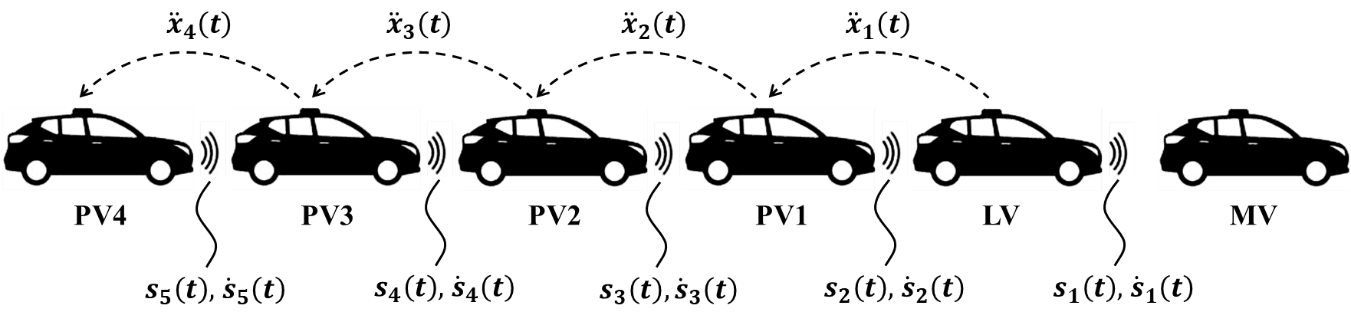
\includegraphics[width=8.5cm]{figs/fig1.png}
  \caption{~Schematic of CACC platoon.}
  \label{fig1}
\end{figure}

Fig.~\ref{fig1} shows a schematic of the CACC platoon, where $s_i (t)$,$\dot{s}_{i} (t)$ indicate the relative gap and relative velocity that CACC obtained through the onboard sensor, and $\ddot{x}_{i-1} (t)$ is the acceleration of the predecessor vehicle obtained through V2V communication.

The CACC design is based on a standard ACC system with a communication module. A CACC platoon can be divided into a Lead Vehicle (LV) and $S-1$ Platoon vehicles (PV)s based on the communication ability of the predecessor vehicle, where $S$ denotes the maximum size of a CACC platoon. Notice that the CACC platoon cannot be infinitely long due to the limitation of the unreliable communication environment. Therefore, we assume the maximum platoon size is the platoon size that can keep communication functioning well. The LVs degrade to ACCs functionally because the predecessor vehicle is an ACC or MV, which cannot communicate, while the communication module of PVs is functioning \citep{dey2015review,navas2019mixing}.

Considering the feasibility of implementation, the controller used in this paper is a decentralized controller instead of a centralized one. The specific information flow topology (IFT) is predecessor following (PF) which means CACCs only communicate with the nearest predecessor to gain further information in advance. As for spacing policy, Constant Time Gap (CTG), including a constant and a velocity-dependent part, is applied due to its widespread use.

\subsection{String stability}
\label{Section 2.2}

We have considered the nuances in different definitions of string stability in the literature. In this paper, the single final string stability is adopted \citep{studli2017vehicular}. Namely, the perturbation only affects the lead vehicle and will not be amplified relative to the response of the last vehicle \citep{qin2021analytical,montanino2021homogeneous,jin2014dynamics,zhou2020stabilizing,wang2018infrastructure}, i.e., between vehicle LV to vehicle PV4 (see Fig.~\ref{fig1}). As for specific spacing policy, the error $e_i (t)$ between the desired and actual inter-vehicle gap is frequently considered in CTG to prevent collisions.

In this paper, the single final string stability of the CACC platoon is studied as a whole instead of analyzing each CACC in the platoon. To facilitate the analysis and focus on the amplification of perturbation, a frequency-domain approach is adopted to obtain a necessary and sufficient condition for the single final string stability of the CACC platoon, which will provide support for designing CACPC.

\subsection{Control Structure}
\label{Section 2.3}
The CACC design is based on a standard ACC system and applies the most commonly used CTG policy. In this subsection, the control structures of the ACC and CACC system are discussed, respectively, to study the subsequent design of CACPC.

It is assumed that each CACC is equipped with i) an on-board radar responsible for collision detection via measuring the gap distance between any two consecutive vehicles, ii) a built-in GPS sensor for measuring the vehicular longitudinal position information, iii) a wireless on-board unit for communicating information of interest with its proximal vehicles via the C-V2X communication, iv) an upper-level controller for calculating the desired longitudinal acceleration based on the parameters obtained, and v) a lower-level controller for determining the throttle and brake actuator inputs so as to track the desired acceleration. Such an assumption is reasonable as the sensing, communication, and actuation units requested above are available in modern CAVs, and thus do not require specific changes in the existing vehicle configuration. Note that the on-board radar only functions when the CACC degrades to the ACC if communication is unavailable or malfunctioning since more accurate information can be obtained faster via communication.

Moreover, we remark that this paper only focuses on homogeneous CACCs where CACCs have the same control structure and controller parameters.


\subsubsection{ACC Control Structure}
\label{Section 2.3.1}
~\\

The primary control object of the ACC system is to maintain the desired gap from the preceding vehicle $s_{d, i}(t)=r_{i}+L_{i}+h_{i} \dot{x}_{i}(t)$, including a velocity-dependent part and a constant part, where $L_i$ represents the vehicle length, $r_i$ is the standstill distance, $x_i$ denotes the longitudinal position of vehicle $i$ and $h_i$ represents the desired time gap of vehicle $i$. Using the onboard sensor, the relative gap $s_{i}(t)=x_{i-1}(t)-x_{i}(t)$ and relative velocity $\dot{s}_{i} (t)$ are measured. In a standard ACC system, the feedback controller controls the error $e_{i}(t)=s_{i}(t)-s_{d, i}(t)$ between the desire gap and relative gap.

The ACC control structure is schematically depicted in Fig.~\ref{fig2} (a).

\begin{figure*}
  \centering
  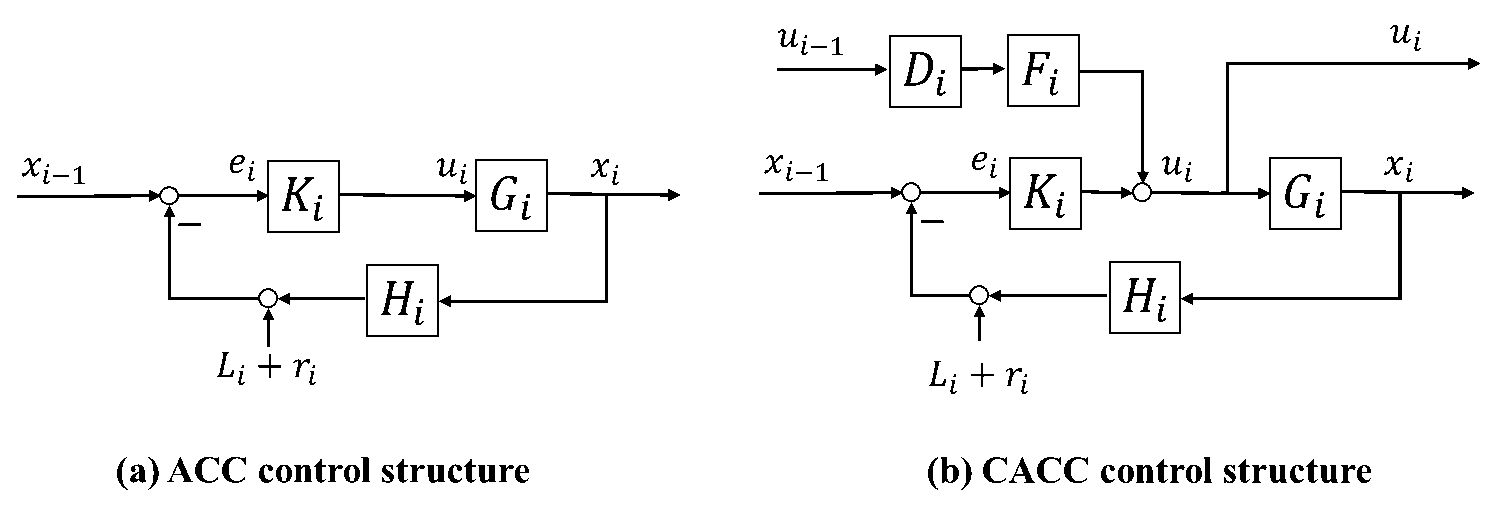
\includegraphics[width=12cm]{figs/fig2.png}
  \caption{~Control structure of ACC and CACC: (a) ACC; (b) CACC.}
  \label{fig2}
\end{figure*}

As shown in Fig.~\ref{fig2} (a), the ACC control structure is represented as a system construction drawing with vehicle position as input and output. The model $K_i (s)$ is the ACC feedback gain, which can be given as:
\begin{equation}
  K_{i}(s)=k_{p}+k_{d} s,
\end{equation}
where $k_p$ is error gain and $k_d$ is error speed gain, the specific parameter setting is based on previous research \citep{milanes2014modeling,milanes2013cooperative}.

The model $G_i (s)$ denotes a lower level controller representing longitudinal vehicle dynamics, where the input $u_i (t)$ of $G_i (s)$ is the desired acceleration derived from $K_i (s)$ and the output $x_i (t)$ is the output position based on the control loop to track desired acceleration through actuation of the throttle and brake system. The linear transfer function of $G_i (s)$ can be represented by \citep{ploeg2013lp}:
\begin{equation}
  G_{i}(s)=\frac{k_{G}}{s^{2}\left(\tau_{i} s+1\right)} e^{-\phi_{i} s},
\end{equation}
where $\tau_{i}^{-1}=\omega_{b w, l, i}$ is the closed-loop bandwidth, $k_G$ is the model gain and $\phi_{i}$ is the time delay of vehicle actuator and intra-vehicle
communication, the specific parameter setting is shown in Table.~\ref{table1} based on the field experiments in Appendix A.

Model $H_i (s)$ is the ACC feedback gain, which can be given as:
\begin{equation}
  H_{i}(s)=1+h_{i} s,
\end{equation}
where $h_i$ is the desired time gap of vehicle i.

The closed-loop transfer function of the ACC system in the frequency domain is as follows:
\begin{equation}
  \mathcal{J}_{i, A C C}(s)=\frac{X_{i}(s)}{X_{i-1}(s)}=\frac{G_{i}(s) K_{i}(s)}{1+H_{i}(s) G_{i}(s) K_{i}(s)},
\end{equation}
where $X_i (s)$ is the Laplace transform of $x_i (t)$.

\subsubsection{CACC Control Structure}
\label{Section 2.3.2}
~\\

As discussed above, the CACC controller is equipped with a communication module that extends the standard ACC feedback controller. The specific control structure is schematically depicted in Fig.~\ref{fig2} (b).

For simplicity, the definitions of model $H_i(s)$, $G_i(s)$, and $K_i(s)$ in the system construction drawing are omitted because they are the same as those in Section.~\ref{Section 2.3.1}. The acceleration $\ddot{x}_{i-1}(t)$ of the predecessor vehicle obtained through V2V communication is used as a feedforward control signal through the feedforward filter $F_i(s)$ and the communication delay model $D_i(s)$.

The model $D_i(s)$ is directly related to the constant communication delay $\theta_i$, which can be expressed as:
\begin{equation}
  D_{i}(s)=e^{-\theta_{i} s},
\end{equation}
where $\theta_i$ represents the constant communication delay. The specific parameter setting is according to previous research \citep{navas2016using,zhang2020control}.

The model $F_i(s)$ is the communication feedforward filter which can be given as:
\begin{equation}
  F_{i}(s)=\left(H_{i}(s) G_{i}(s)\right)^{-1}.
\end{equation}

The closed-loop transfer function of the CACC system in the frequency domain is as follows:
\begin{equation}
  \mathcal{J}_{i, C A C C}(s)=\frac{X_{i}(s)}{X_{i-1}(s)}=\frac{\left(K_{i}(s)+D_{i}(s) F_{i}(s)\right) G_{i}(s)}{1+H_{i}(s) G_{i}(s) K_{i}(s)}.
\end{equation}

\subsubsection{CACPC structure}
\label{Section 2.3.3}
~\\
\begin{figure*}
  \centering
  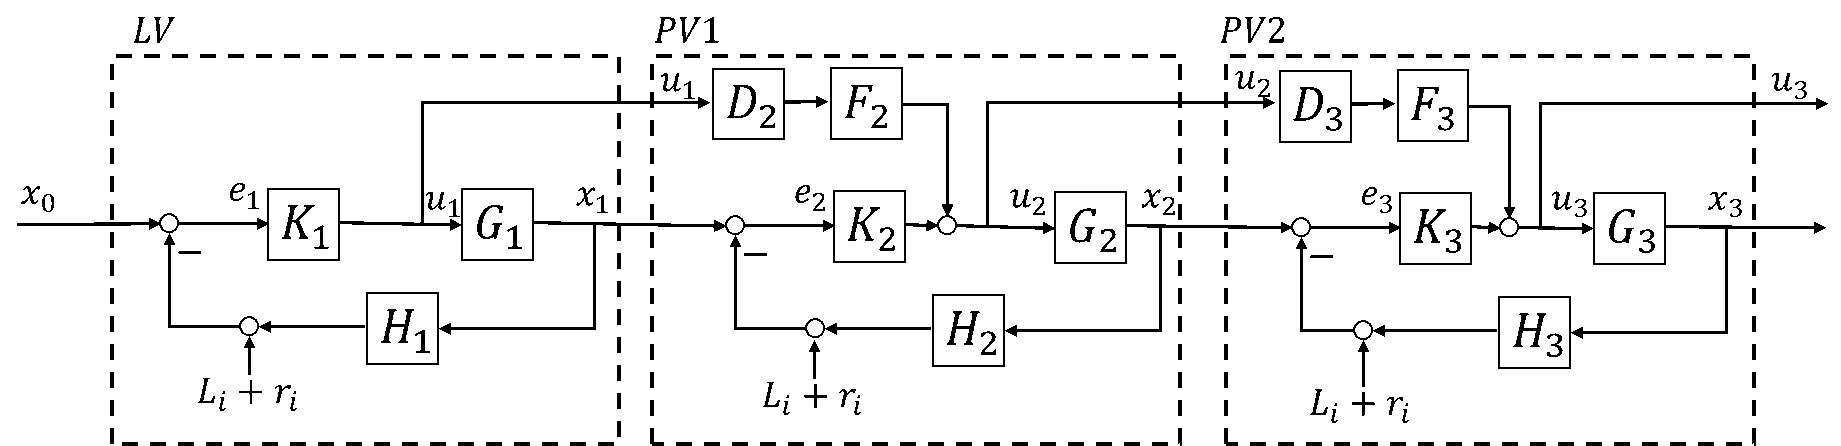
\includegraphics[width=14cm]{figs/fig3.png}
  \caption{~CACPC structure.}
  \label{fig3}
\end{figure*}

As the control system for the controller design in this paper, the CACC platoon is designated as the primary control unit for string stability analyses. We can couple the control structure of ACC and CACC by merging the inner and outer signals, thus establishing the structure of CACPC. The specific structure of the CACPC is schematically depicted in Fig.~\ref{fig3}.

For simplicity, the definitions of model $H_i(s)$, $G_i(s)$, $K_i(s)$ and $D_i(s)$ in system construction drawing are omitted because they are the same as those in Section.~\ref{Section 2.3.1} and ~\ref{Section 2.3.2}.

The closed-loop transfer function of CACPC system in the frequency domain is as follows:
\begin{equation}
  \begin{aligned}
    \mathcal{J}_{\text {platoon }}(s)
     & =\frac{X_{n}(s)}{X_{0}(s)}=\frac{X_{n}(s)}{X_{n-1}(s)} \frac{X_{n-1}(s)}{X_{n-2}(s)} \ldots \frac{X_{1}(s)}{X_{0}(s)} \\
     & =\mathcal{J}_{1, A C C}(s) \prod_{i=2}^{n} \mathcal{J}_{i, C A C C}(s),
  \end{aligned}
  \label{Eq8}
\end{equation}
where $n$ denotes the platoon size.

\section{Methodology}
\label{Section 3}
In this section, the primary methodology applied in this paper is introduced, including the transfer function method for string stability analyses and the YK parameterization for controller switching.

\subsection{String stability analysis}
\label{Section 3.1}

Laplace transform is a classic method to explore string stability in a direct and precise manner. Moreover, it has been adopted in extensive research \citep{orosz2011delayed,montanino2021string,feng2019string}. Therefore, single final string stability analyses of this paper are conducted based on the Laplace transform. The relationship of the perturbation propagating through the CACC platoon in the frequency domain is:
\begin{equation}
  \mathcal{J}_{\text {platoon }}(s)=\frac{X_{n}(s)}{X_{0}(s)}.
\end{equation}

According to the definition of string stability, a sufficient and necessary conservative condition for string stability can be derived according to the $\mathcal{L}_{\infty}$ norm:
\begin{equation}
  \left\|x_{n}(t)\right\|_{\mathcal{L}_{\infty}} \leq \left\|x_{0}(t)\right\|_{\mathcal{L}_{\infty}}
  % \left\|\mathcal{J}_{\text {platoon }}(s)\right\|_{\mathcal{H}_{\infty}} \leq 1.
  \label{Eql_inf}
\end{equation}
where $x_{n}(t)$ and $x_{0}(t)$ are the inverse Laplace transformation of $X_{n}(s)$ and $X_{0}(s)$, respectively; $\|.\|_{\mathcal{L}_{\infty}}$ is the $\mathcal{L}_{\infty}$ norm, which deals with the peak of perturbations.

Moreover, according to the relationship $\|g\|_{1}=\sup _{x \in L_{\infty}} \frac{\|y\|_{\mathcal{L}_{\infty}}}{\|x\|_{\mathcal{L}_{\infty}}}$ Equation(\ref{Eql_inf}) can be replaced as:
\begin{equation}
  \|j\left(t\right)\|_{1}\leq 1
  \label{Eql_inf2}
\end{equation}
where $j\left(t\right)$ denotes the impulse response of $\mathcal{J}_{\text {platoon }}(s)$.

Furthermore, the Equation(\ref{Eql_inf2}) can be replaced by the following two conditions \citep{Swaroop1994}:
\begin{equation}
  \|\mathcal{J}_{\text {platoon }}(s)\|_{\infty} \leq 1 \quad \& \quad j\left(t\right)>0
  \label{Eql_inf3}
\end{equation}

We remark that we adopt $\mathcal{L}_{\infty}$ norms of the string stability instead of $\mathcal{L}_{2}$ norms. Although $\mathcal{L}_{2}$ norms can provide more explicit derivation, it only deals with the energy dissipation in the upstream direction and not the peak of perturbations \citep{Darbha2003}. In addition, the single final string stability is adopted in this paper for string stability analyses since it can deal with the relationship between peaks of perturbation before and after it spreads over the platoon. So that the string stability indicates the perturbation is not amplified by the CACC platoon \citep{Studli2017}.
% Meanwhile, if $s=j\omega$, according to the definition of Laplace transform, we have:
% \begin{equation}
%   \left\|\mathcal{J}_{\text {platoon }}(j \omega)\right\|_{\mathcal{H}_{\infty}} \leq 1.
% \end{equation}

% Based on the transfer function of CACPC Equation(\ref{Eq8}), the following relation can be derived from linear system theory:
% \begin{equation}
%   \left\|\mathcal{J}_{\text {platoon }}(j \omega)\right\|_{\mathcal{H}_{\infty}}=\left\|\mathcal{J}_{1, A C C}(j \omega) \prod_{i=2}^{n} \mathcal{J}_{i, C A C C}(j \omega)\right\|_{\mathcal{H}_{\infty}}=\max _{x_{0} \neq 0} \frac{\left\|x_{n}(t)\right\|_{\mathcal{L}_{2}}}{\left\|x_{0}(t)\right\|_{\mathcal{L}_{2}}} \leq 1,
%   \label{Eq12}
% \end{equation}
% where $\mathcal{J}_{platoon}(j\omega)$ is the transfer function of CACC platoon evaluated on imaginary axis, $\|.\|_{\mathcal{H}_{\infty}}$ is the $\mathcal{H}_{\infty}$ norm, which means the supremum of $\mathcal{J}_{platoon}(j\omega)$ for all $\omega$, and$\|. \|_{\mathcal{L}_{2}}$ is the $\mathcal{L}_{2}$ norm.

% This condition can be interpreted as requiring energy dissipation in the upstream direction. This follows from the fact that, according to Equation(\ref{Eq12}), the $\mathcal{H}_{\infty}$ norm is induced by the $\mathcal{L}_{2}$ norms of input and output, which, in turn, measure for energy. We remark that we adopt $\mathcal{L}_{2}$ norms of the string stability instead of $\mathcal{L}_{\infty}$ norms. Although

\subsection{Controller switching method: Youla-Kucera parametrization}
\label{Section 3.2}

Maintaining string stability of the CACC platoon is one of the primary control objectives. However, this control objective is difficult for the CACC platoon with variable platoon size because it implies a compromise between string stability and capacity. Therefore an adaptive controller design approach for platoon size is needed to maintain string stability while maximizing capacity. Besides, adapting to the platoon size leads to another problem: the controller switching when the platoon size changes. Direct controller switching is a transient process that is chaotic, meaning that the intermediate states do not necessarily remain stable even if the controllers are stable before and after switching. Moreover, controller switching will inevitably trigger endogenous perturbations, which will cause safety hazards in the traffic flow. Therefore, a parameterization method for smooth switching between different controllers is needed to ensure the feasibility of the above CACC controllers design.

Youla-Kucera (YK) parametrization is a method to stabilize the class of a given plant that contains all stabilizing controllers \citep{dasgupta1996parametrization,navas2017youla}. One of the advantages of this method is that the performance transfer function is tuned with a particular parameter, which means that the stability of unstable open-loop controllers can be maintained while switching between controllers. It is worth noting that the switching controller designed using YK parametrization is a controller class consisting of a set of stabilizing controllers based on a tuning function and a parameter. Therefore, the YK parametrization can transform the controller switch into a change in the tuning function and thus avoid strong endogenous perturbations due to direct changes in the controller.

The basis of YK parametrization is described in detail below, which includes doubly coprime factorization and YK parameterization of all stabilizing controllers.

Basic notations are introduced below. $\mathbb{R} H_{\infty}$ is the real stable transfer function space; $G$ and $K_i$ maintain the same definitions as in Section.~\ref{Section 3}.

\subsubsection{Fundamentals on YK parametrization}
\label{Section 3.2.1}
~\\


Before applying YK parametrization, the internal dynamics of the vehicles $G$ need to be presented as state-space representation for subsequent analyses:
\begin{equation}
  \begin{gathered}
    \dot{m}(t)=A m(t)+B u(t) \\
    x(t)=C m(t)+D u(t)
  \end{gathered}, G(s)=\left[\begin{array}{ll}
      A & B \\
      C & D
    \end{array}\right],
\end{equation}
where $t$ indicates time, $m(t)$ is the state vector, $\dot{m}(t)$ is the evolution of the state vector over time, $x(t)$ is the output vector, and $u(t)$ is the control vector. $A$, $B$, $C$, and $D$ are the constant coefficients matrices of state-space matrices of $G$.

Then any appropriate controller $K_i$ could stabilize this system, which is represented as:
\begin{equation}
  \begin{gathered}
    \dot{n}(t)=A_{i}^{c} n(t)+B_{i}^{c} e(t) \\
    u(t)=C_{i}^{c} n(t)+D_{i}^{c} e(t)
  \end{gathered}, K_{i}(s)=\left[\begin{array}{ll}
      A_{i}^{c} & B_{i}^{c} \\
      C_{i}^{c} & D_{i}^{c}
    \end{array}\right],
\end{equation}
where $n(t)$ is the state vector, and $A_i^c$,$B_i^c$,$C_i^c$ and $D_i^c$ are the constant coefficients matrices of state-space matrices of $K_i$. Note that we choose $K_0$ represents the initial controller, and $K_1$ represents the controller after a complete switch.

\subsubsection{Doubly coprime factorization}
\label{Section 3.2.2}
~\\

Double coprime factorization is one of the keys to YK parameterization. Coprime factors are obtained by coprime factorization of the plant and controllers. Then the stabilizing controller class corresponding to the plant $G$ can be derived through interpolation. In this process, factorization means the plant and controllers are represented as the products of two transfer functions. Coprimeness refers to the absence of common zeros in the right half-plane, and double coprimeness excludes unstable pole/zero cancellations and refers to the idea of being right and left coprime.

The coprime factors of $G$ and $K_i$ can be expressed as:
\begin{equation}
  G=N M^{-1}=\tilde{M}^{-1} \tilde{N}, K_{i}=U_{i} V_{i}^{-1}=\tilde{V}_{i}^{-1} \tilde{U}_{i},
\end{equation}
where coprime factors $N, M, \tilde{M}, \tilde{N}, U_{i}, V_{i}, \tilde{U}_{i}, \tilde{V}_{i} \in \mathbb{R} H_{\infty}$ satisfy double Bezout's identity \citep{pommaret1998generalized}:
\begin{equation}
  \begin{aligned}
    \left[\begin{array}{cc}
        \tilde{V}_{i} & -\tilde{U}_{i} \\
        -\tilde{N}    & \tilde{M}
      \end{array}\right]\left[\begin{array}{cc}
        M & U_{i} \\
        N & V_{i}
      \end{array}\right]
     & =\left[\begin{array}{cc}
        M & U_{i} \\
        N & V_{i}
      \end{array}\right]\left[\begin{array}{cc}
        \tilde{V}_{i} & -\tilde{U}_{i} \\
        -\tilde{N}    & \tilde{M}
      \end{array}\right] \\
     & =\left[\begin{array}{cc}
        I & 0 \\
        0 & I
      \end{array}\right].
  \end{aligned}
  \label{Eq16}
\end{equation}

Using the relationship of state-space representation and transfer function $G(s)=C(sI-A)^{-1} B$ and $K_i (s)=C_i^c (sI-A_i^c)^{-1} B_i^c+D_i^c$, coprime factors can be expressed by:
\begin{equation}
  \left[\begin{array}{cc}
      M & U_{i} \\
      N & V_{i}
    \end{array}\right]=\left[\begin{array}{cc|cc}
      A+B F     & 0                             & -B & 0         \\
      0         & A_{i}^{c}+B_{i}^{c} F_{i}^{c} & 0  & B_{i}^{c} \\
      \hline -F & C_{i}^{c}+D_{i}^{c} F_{i}^{c} & I  & D_{i}^{c} \\
      -C        & F_{i}^{c}                     & 0  & I
    \end{array}\right],
  \label{Eq17}
\end{equation}
\begin{equation}
  \left[\begin{array}{cc}
      \tilde{V}_{i} & -\tilde{U}_{i} \\
      -\tilde{N}    & \tilde{M}
    \end{array}\right]=\left[\begin{array}{cc|cc}
      A+B  D_{i}^{c} C          & B  C_{i}^{c} & -B & B  D_{i}^{c} \\
      B_{i}^{c} C               & A_{i}^{c}    & 0  & B_{i}^{c}    \\
      \hline F_{i}- D_{i}^{c} C & -C_{i}^{c}   & I  & -D_{i}^{c}   \\
      C                         & -F_{i}^{c}   & 0  & I            \\
    \end{array}\right],
  \label{Eq18}
\end{equation}
where $F$ and $F_i^c$ should be chosen such that $A+BF$,$A_i^c+B_i^c F_i^c\in \mathbb{R} H_{\infty}$. Straight lines indicate the elements of the matrix that belong to each factor respectively. The proof of the Equation (\ref{Eq17}-\ref{Eq18}) is detailed in Appendix B.

Note that only the controller switches from $K_0$ to $K_1$ during the process of controller switching, and the internal dynamics of the vehicles $G$ remain unchanged. Therefore, the coprime factors of $G$ ($M$ and $N$) remain unchanged while the coprime factors of $K_0$ ($U_0$, $V_0$) and $K_1$ ($U_1$, $V_1$) are switching.

\subsubsection{YK parameterization of all stabilizing controllers}
\label{Section 3.2.3}
~\\

The most critical step of YK parameterization is to establish a controller class containing all controllers that can stabilize a given plant $G$ through a parameter $Q$ based on coprime factors of the plant $G$ and controllers $K_i$ before and after switching. Through controller interpolation, the expressions of $K(Q)$ and $Q$ are derived as:
\begin{equation}
  \begin{aligned}
    K(Q) & =  \left(U_{0}+M \gamma Q\right)\left(V_{0}+N \gamma Q\right)^{-1}                                                                     \\
         & =\left(\tilde{V}_{0}+\gamma Q \tilde{N}\right)^{-1}\left(\tilde{U}_{0}+\gamma Q \tilde{M}\right), Q \in \mathbb{R} H_{\infty}^{p x m},
  \end{aligned}
\end{equation}
\begin{equation}
  Q=\tilde{U}_{1}-\tilde{V}_{1} \tilde{V}_{0}^{-1} \tilde{U}_{0},
  \label{Eq20}
\end{equation}
where $\gamma \in [0,1]$ is a scalar factor playing a pivotal role as a switching signal in controller interpolation, indicating the level of interconnection of the two controllers \citep{niemann1999architecture}. When $\gamma=0$, the controller is completely taken over by $K_0$, while $K_1$ is fully controlled when $\gamma=1$.

\textbf{Proof:} First, check the matrix of the closed-loop feedback control system.

\begin{equation}
  \begin{aligned}
     & \left[\begin{array}{cc}
        I  & -K(Q) \\
        -G & I
      \end{array}\right]^{-1}                                                                                                                                                              \\
     & =\left[\begin{array}{cc}
        I                         & -(\tilde{V}_{0}+\gamma Q \tilde{N})^{-1} (\tilde{U}_{0}+\gamma Q \tilde{M}) \\
        -\tilde{M}^{-1} \tilde{N} & I
      \end{array}\right]^{-1}                                                                                                                                                             \\
     & =\left\{\left[\begin{array}{cc}
        (\tilde{V}_{0}+\gamma Q \tilde{N})^{-1} & 0              \\
        0                                       & \tilde{M}^{-1}
      \end{array}\right]\left[\begin{array}{cc}
        \tilde{V}_{0}+\gamma Q \tilde{N} & -(\tilde{U}_{0}+\gamma Q \tilde{M}) \\
        -\tilde{N}                       & \tilde{M}
      \end{array}\right]\right\}^{-1}                                                                                                   \\
     & =\left[\begin{array}{cc}
        M & U_{0}+M \gamma Q \\
        N & V_{0}+N \gamma Q
      \end{array}\right]\left[\begin{array}{cc}
        \tilde{V}_{0}+\gamma Q \tilde{N} & 0         \\
        0                                & \tilde{M}
      \end{array}\right]                                                                                                                       \\
     & =\left\{\left[\begin{array}{ll}
        M & U \\
        N & V
      \end{array}\right]+\left[\begin{array}{ll}
        0 & \gamma M Q \\
        0 & \gamma N Q
      \end{array}\right]\right\}\left\{\left[\begin{array}{cc}
        \tilde{V} & 0         \\
        0         & \tilde{M}
      \end{array}\right]+\left[\begin{array}{cc}
        \gamma Q \tilde{N} & 0 \\
        0                  & 0
      \end{array}\right]\right\} \\
     & =\left[\begin{array}{cc}
        M & U \\
        N & V
      \end{array}\right]\left[\begin{array}{cc}
        \tilde{V} & 0         \\
        0         & \tilde{M}
      \end{array}\right]+\left[\begin{array}{cc}
        \gamma M Q \tilde{N} & 0 \\
        \gamma N Q \tilde{N} & 0
      \end{array}\right]+\left[\begin{array}{cc}
        0 & \gamma M Q \tilde{M} \\
        0 & \gamma N Q \tilde{M}
      \end{array}\right]                               \\
     & =\left[\begin{array}{cc}
        \tilde{V}  & -\tilde{U} \\
        -\tilde{N} & \tilde{M}
      \end{array}\right]^{-1}\left[\begin{array}{cc}
        \tilde{V}^{-1} & 0              \\
        0              & \tilde{M}^{-1}
      \end{array}\right]^{-1}+\left[\begin{array}{cc}
        \gamma M Q \tilde{N} & \gamma M Q \tilde{M} \\
        \gamma N Q \tilde{N} & \gamma N Q \tilde{M}
      \end{array}\right]                                                                 \\
     & =\left[\begin{array}{cc}M & U \\ N & V\end{array}\right]\left[\begin{array}{cc}\tilde{V} & 0 \\ 0 & \tilde{M}\end{array}\right]+\left[\begin{array}{c}M \\ N\end{array}\right] \gamma Q\left[\begin{array}{cc}\tilde{N} & \tilde{M}\end{array}\right]                       \\
     & =\left[\begin{array}{cc}
        I  & -K \\
        -G & I
      \end{array}\right]^{-1}+\left[\begin{array}{c}
        M \\
        N
      \end{array}\right] \gamma Q\left[\begin{array}{cc}
        \tilde{N} & \tilde{M}
      \end{array}\right] \in \mathbb{R} H_{\infty}^{p x m}.
  \end{aligned}
  \label{Eq App C}
\end{equation}

From Equation (\ref{Eq App C}), it is clearly that any controller $K(Q)$ parameterized by $Q \in \mathbb{R} H_{\infty}^{p x m} $ stabilizes the plant $G$ according to the Corollary 4.2 in references \citep{tay1998high,MAHTOUT202081}.

In addition, the factors affecting the functioning controllers during switching contain only the tuning function $\gamma$ and coprime factors of the plant $G$ and controllers $K_i$. Since the plant $G$ and controllers $K_i$ do not change in the switching process, their coprime factors do not change either. Therefore, during controllers switching, the functioning controllers included in the controller family $K(Q)$ are only affected by the tuning function $\gamma$. Moreover, the closed-loop poles of the system during the switching process are the combination of $[G, K_0]$ and $[G, K_1]$, which can maintain the stability of the system under any combination of $Q$ and $\gamma$, thus ensuring the stable switch of the controllers independent of $\gamma$ \citep{niemann1999architecture}.


\section{YK parameterization}
\label{Section 4}
In this section, the detailed controller design process is carried out using the methodology proposed in Section.~\ref{Section 3}. Specifically, the CACC platoon controller design process based on YK parameterization includes:
\begin{enumerate}
  \item Selecting the desired time gap before and after the controller switching based on string stability analyses;
  \item Modifying the control structure proposed in Section.~\ref{Section 2.3} to YK control structure and calculating the coprime factors of the controllers before and after switching and YK parameters $Q$;
  \item Determining the tuning function $\gamma$ for different platoon sizes according to the string stability analyses results and YK control structure in Section.~\ref{Section 4.2}.
\end{enumerate}

In addition, to facilitate subsequent calculations and experiments, the above-defined controller coefficients selected in this paper are as follows, which are set based on existing research \citep{navas2016using,milanes2014modeling,milanes2013cooperative} and field experiments employed detailed in Appendix A. The specific parameter setting is shown in Table.~\ref{table1}. Moreover, the maximum platoon size $S$ of the CACC platoon is set to 5 in the paper, which is absolutely feasible and effective for communication latency and packet loss rates from the perspective of the communication technology.
\begin{table}
  \centering

  \setlength{\abovecaptionskip}{0pt}
  \setlength{\belowcaptionskip}{10pt}%设置标题与表格的距离
  \caption{~Parameters chosen for ACC and CACC controller.}
  \resizebox{.95\columnwidth}{!}
  {\begin{tabular}{lcccccc} \toprule
      Parameter & $k_{p}$ & $k_{d}$ & $\tau_{i}$ & $k_{G}$ & $\phi_{i}$ & $\theta_{i}$ \\ \midrule Value & $0.45$ $ \mathrm{s}^{-2}$ & $0.25 $ $ \mathrm{s}^{-1}$ & $0.7862 \mathrm{~s} / \mathrm{rad}$ & $0.9403$ & $0.2 \mathrm{~s}.$ & $0.3 \mathrm{~s}$ \\ \bottomrule
      \label{table1}
    \end{tabular}}

\end{table}

\subsection{Analyses of string stability}
\label{Section 4.1}

When the CACC platoon is formed, taking the CACC platoon as the control object can maintain a smaller desired time gap without losing string stability. Note that the CACC platoon contains the lead ACC (which is a CACC but degraded to an ACC functionally) and several CACCs, the desired time gaps of the ACC and CACCs are different. Therefore, we need to investigate not only the minimum desired time gaps of the ACC and CACCs but also the minimum desired time gap combination for the CACC platoon. The corresponding theoretical analyses regarding string stability are carried out using the method proposed in Section.~\ref{Section 3.1}.

As for the desired time gap $h_i=h_{i,min}$, margin string stability criterion (\ref{Eql_inf3}) is met, and string stability can be guaranteed when $h_i\ge h_{i,min}$ \citep{naus2010string}. However, due to the complexity of the CACPC structure, the calculation of the minimum desired time gap $h_{i,min}$ is too complicated and cannot give an algebraic equation of $h_{acc}$ and $h_{cacc}$, so the derivation is not discussed here. A numerical approximation approach is adopted to explore the combination of $h_{min,acc}$ and $h_{min,cacc}$ as margin string stable according to Equation (\ref{Eql_inf3}). Moreover, since the perturbation faced in real traffic conditions is considered to be of infinite wavelength \citep{bian2019reducing,xiao2011practical}, we only focus on the magnitude of the transfer function under low frequency ($10^{-5} - 10^0$ Hz) \citep{Oncu2014}. Fig.~\ref{fig4} shows that $h_{min,cacc}$ changes with $h_{min,acc}$ over different frequencies where the heatmap shows the margin stable combination of $h_{min,cacc}$ and $h_{min,acc}$ under different perturbation frequency and the colored contour lines represent the stability demarcation lines of the combination of $h_{min,cacc}$ and $h_{min,acc}$ under perturbation frequency.

\begin{figure*}
  \centering
  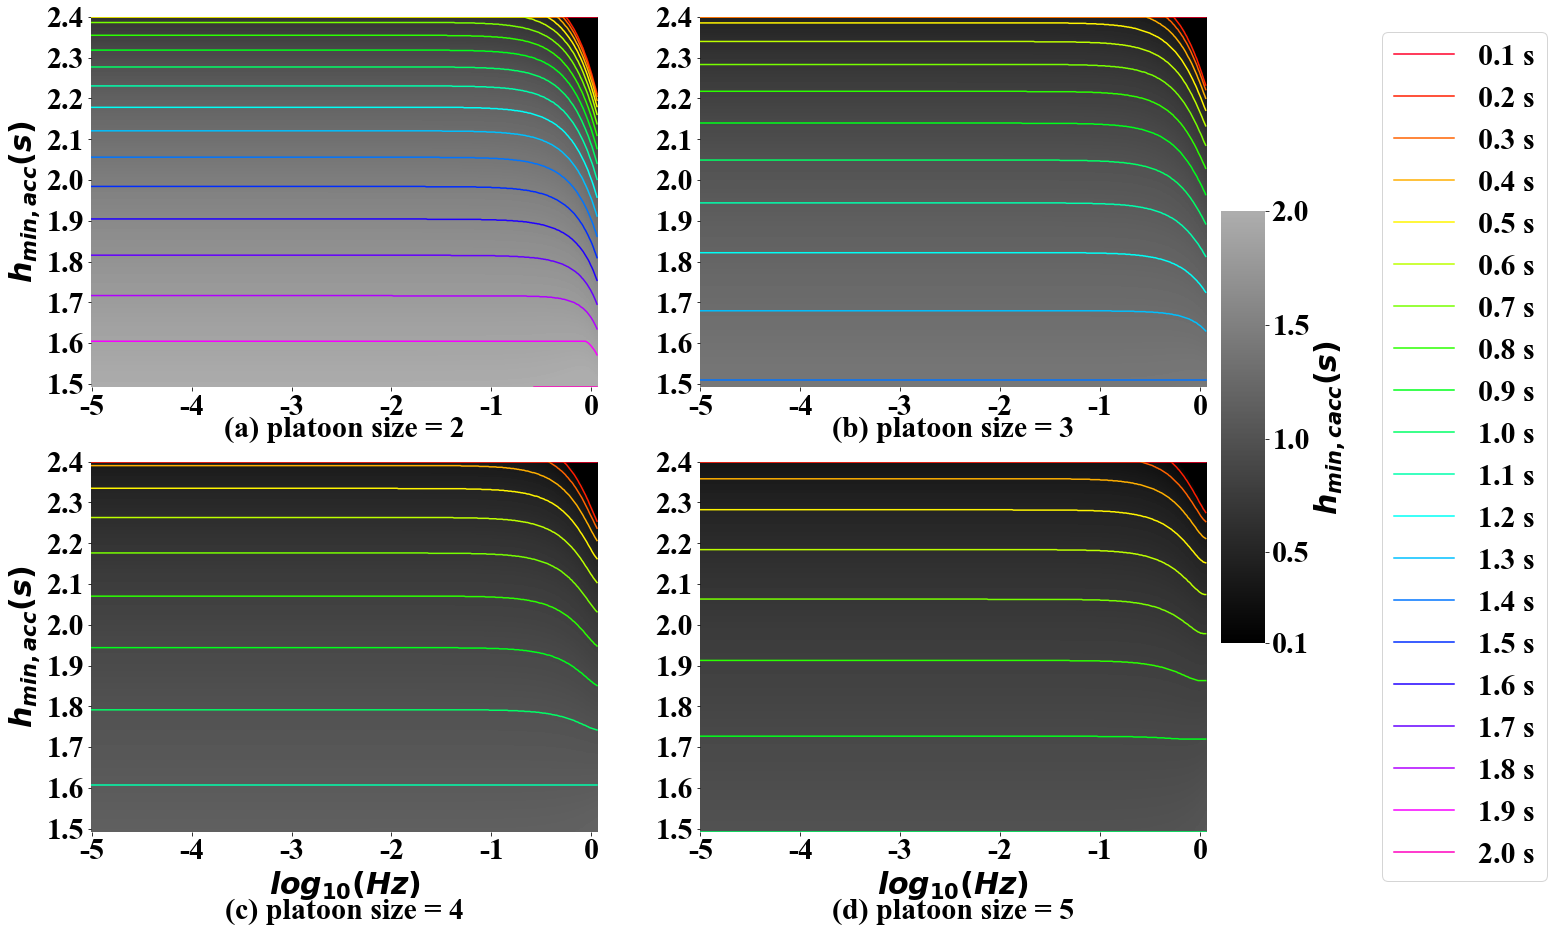
\includegraphics[width=14cm]{figs/fig4.png}
  \caption{~Contour plot of perturbation frequency versus $h_{min,acc}$, indicating the corresponding minimal value for $h_{min,cacc}$.}
  \label{fig4}
\end{figure*}

It can be clearly found in Fig.~\ref{fig4} that CACC can maintain a smaller desired time gap with platoon size increasing. Moreover, $h_{min,cacc}$ can significantly decrease with $h_{min,acc}$ increasing, which means the feasibility of eliminating the redundancy within the CACC platoon through the appropriate deployment of the desired time gap. In addition, string stability can be significantly improved as the frequency of perturbation approaches $10^0$ Hz, which is represented as the arc under $10^{-0.5} - 10^0$ Hz in Fig.~\ref{fig4}. When we focus on the region of $10^{-5} - 10^{-0.5}$ Hz, an interesting phenomenon is discovered that $h_{min,cacc}$ stays the same as the frequency increases, which means the combination of $h_{min,cacc}$ and $h_{min,acc}$ to guarantee the string stability is determined for a specific platoon size.

Based on the conclusions obtained above, in order to maximize the capacity while ensuring string stability and safety, we choose $h_{1,acc}=2s$ and $h_{1,cacc}=0.4s$ for the case of $S=5$ which indicates the controller after switching while the desired time gap settings of ACC and CACC for the case of $S=2$ are $h_{0,acc}=2.108s$ and $h_{0,cacc}=0.747s$ adopted by the controller before switching in this paper.

\subsection{Analyses of controller switching}
\label{Section 4.2}

Based on the combination of the minimum desired time gap obtained in Section.~\ref{Section 4.1}, the controller can be determined. Then the control structures proposed in Section.~\ref{Section 2.3} need to be modified to the equivalent YK control structures. In addition, the coprime factors of the controllers and the YK parameters $Q$ can be derived.

\subsubsection{Modify ACC controller}
\label{Section 4.2.1}
~\\

For the LV in a CACC platoon, since it cannot communicate with the predecessor vehicle, it loses the information gained from the communication module, so its control system is represented by standard ACC, as shown in Fig.~\ref{fig2} (a).

To incorporate the desired time gap into the controller, the ACC controller in Fig.~\ref{fig2} (a) is reconstructed so that the ACC controller can perform stable interpolation for the different desired time gaps $h_i$. Moreover, the corresponding equivalent ACC control structure is shown in Fig.~\ref{fig5}. The transfer function of the extended controller is as follows:
\begin{equation}
  K_{e x t, a c c}^{i}(s)=\frac{K_{i}}{1+h_{i} G_{i} K_{i} s}.
\end{equation}
\begin{figure}
  \centering
  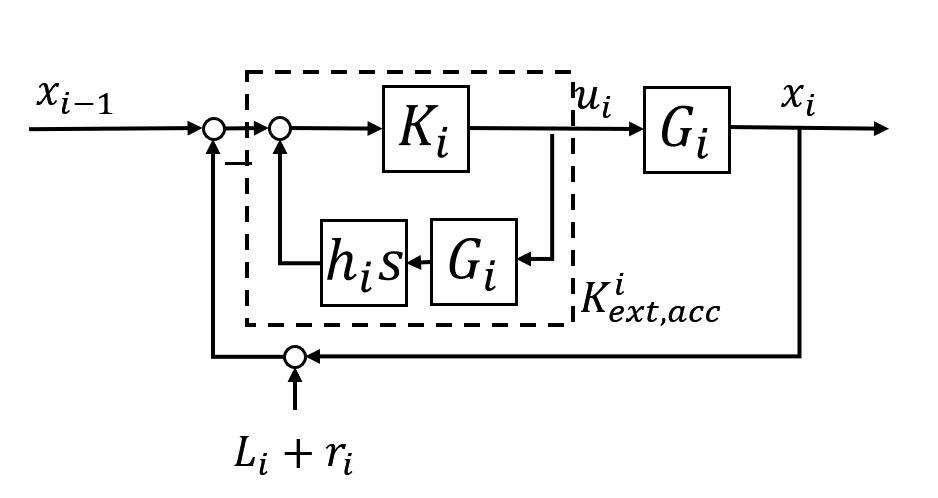
\includegraphics[width=6.5cm]{figs/fig5.png}
  \caption{~Equivalent ACC control structure.}
  \label{fig5}
\end{figure}

\subsubsection{YK parametrization for ACC controller}
\label{Section 4.2.2}
~\\

Based on the mathematical basis introduced in Section.~\ref{Section 3.2}, the control structure applied to controller switching needs to be modified accordingly by introducing a dual coprime factor. The control structure for switching based on left coprime factors is shown in Fig.~\ref{fig6}:

\begin{figure}
  \centering
  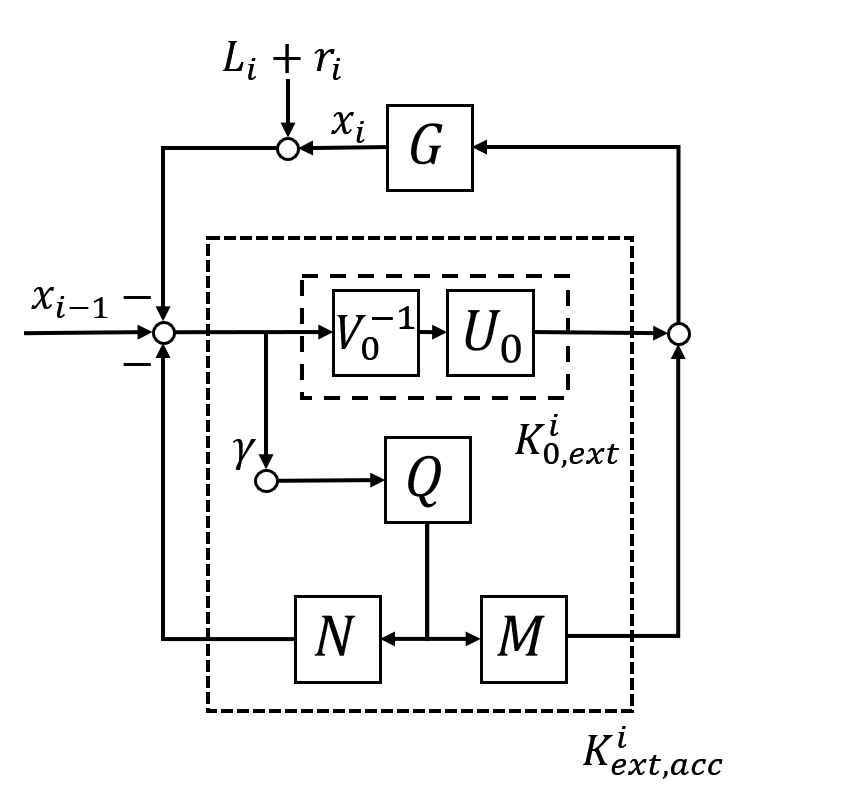
\includegraphics[width=6cm]{figs/fig6.png}
  \caption{~YK control structure for ACC controllers switching.}
  \label{fig6}
\end{figure}
For stable switching purposes, coprime factors need to meet double Bezout's identity as shown in Equation (\ref{Eq16}) based on the state-space matrix of transfer functions of $K_{0,acc}$, $K_{1,acc}$. In addition, the minimum desired time gap of the controllers before and after switching determined in Section.~\ref{Section 4.1} is adopted for determining the specific controller. Then the specific transfer function equations for the coprime factors of $K_{0,acc}$ and $K_{1,acc}$ are as follows:
\begin{equation}
  \begin{aligned}
     & U_{0}=\frac{-s(s+1.272)(s+1.8)}{(s+4.42)\left(s^{2}+1.836 s+1.027\right)},                 \\
     & V_{0}=\frac{-4\left(s^{2}+1.902 s+1.135\right)}{(s+4.42)\left(s^{2}+1.836 s+1.027\right)}, \\
     & U_{1}=\frac{-s(s+1.272)(s+1.8)}{(s+4.42)\left(s^{2}+1.808 s+0.9741\right)},                \\
     & V_{1}=\frac{-4\left(s^{2}+1.87 s+1.076\right)}{(s+4.42)\left(s^{2}+1.808 s+0.9741\right)}.
  \end{aligned}
\end{equation}
As for the YK parameter $Q_{acc}$, substitute coprime factors into Equation(\ref{Eq20}):

\begin{small}
  \begin{equation}
    \begin{gathered}
      \begin{aligned}
                   & \quad -0.1005(s+1.892)(s+4.38)(s+4.42)                                                                                                                      \\
        Q_{a c c}= & \frac{\left(s^{2}+1.82 s+0.9968\right)\left(s^{2}+1.969 s+1.238\right)}{(s+4.42)^{3}\left(s^{2}+1.808 s+0.9741\right)\left(s^{2}+1.836 s+1.027\right)^{2}}.
      \end{aligned}
    \end{gathered}
  \end{equation}
\end{small}

\subsubsection{Modify CACC controller}
\label{Section 4.2.3}
~\\

Similar to the method adopted in Section.~\ref{Section 4.2.1}, the system construction drawing of the CACC controller is in Fig.~\ref{fig3}, which is reconstructed to incorporate the desired time gap $h_i$ into the controller. Furthermore, the corresponding equivalent CACC control structure is shown in Fig.~\ref{fig7}. The transfer function of the extended controller is as follows:

\begin{equation}
  K_{e x t, c a c c}^{i}(s)=\frac{K_{i}}{1+h_{i} G_{i} K_{i} s}.
\end{equation}

\begin{figure}
  \centering
  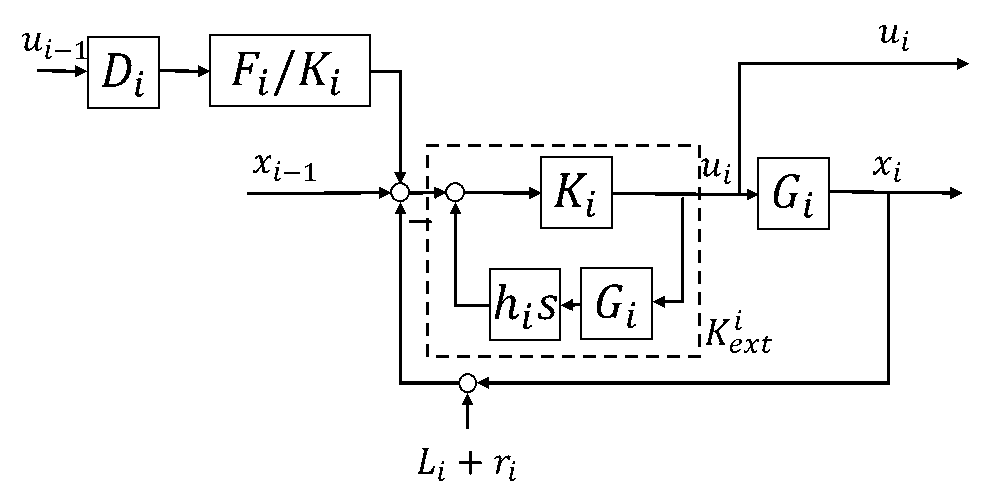
\includegraphics[width=8.5cm]{figs/fig7.png}
  \caption{~Equivalent CACC control structure.}
  \label{fig7}
\end{figure}

\subsubsection{YK parametrization for CACC controller}
\label{Section 4.2.4}
~\\

Similar to Section.~\ref{Section 4.2.2}, the control structure applied to controller switching needs to be modified accordingly by introducing a dual coprime factor based on the mathematical basis presented in Section.~\ref{Section 3.2}. The control structure for switching based on left coprime factors is shown in Fig.~\ref{fig8}:

\begin{figure}
  \centering
  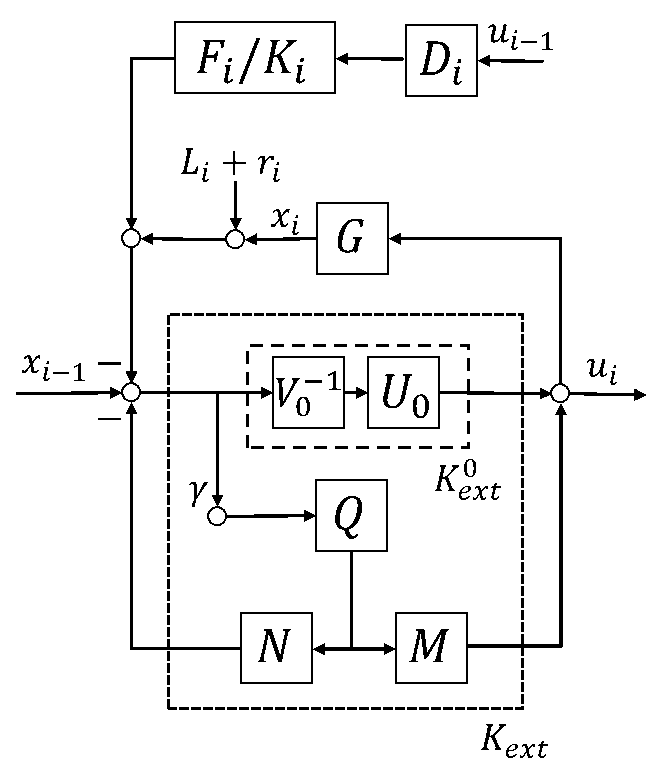
\includegraphics[width=6cm]{figs/fig8.png}
  \caption{~YK control structure for CACC controllers switching.}
  \label{fig8}
\end{figure}

Based on Equation (\ref{Eq17}-\ref{Eq18}), coprime factors which meet double Bezout's identity, as shown in Equation (\ref{Eq16}), can be obtained easily. The minimum desired time gap of the controllers before and after switching determined in Section.~\ref{Section 4.1} is adopted. Then the specific transfer function equations for the coprime factors of $K_{0,cacc}$ and $K_{1,cacc}$ are as follows:
\begin{equation}
  \begin{aligned}
     & U_{3}=\frac{-s(s+1.272)(s+1.8)}{(s+4.406)(s+1.159)(s+0.3148)},    \\
     & V_{3}=\frac{-4(s+1.144)(s+0.3515)}{(s+4.406)(s+1.159)(s+0.3148)}, \\
     & U_{4}=\frac{-s(s+1.272)(s+1.8)}{(s+4.397)(s+1.226)(s+0.1438)},    \\
     & V_{4}=\frac{-4(s+1.221)(s+0.1587)}{(s+4.397)(s+1.226)(s+0.1438)}.
  \end{aligned}
\end{equation}
As for the YK parameter $Q_{cacc}$, substitute coprime factors into Equation(\ref{Eq20}):
% \begin{small}
%     \begin{equation}
%         \begin{gathered}
%             \begin{aligned}
%         Q_{c a c c}=\frac{-0.4451(s+4.402)(s+3.51)(s+1.918)(s+1.8)(s+1.274)(s+1.219)(s+1.414)(s+0.3596)(s+0.1572)}{(s+4.397)(s+1.8)(s+1.272)(s+1.226)(s+0.1438)(s+4.406)^{2}(s+0.3148)^{2}\left(s^{2}+2.319 s+1.344\right)}.
%             \end{aligned}
%         \end{gathered}
%     \end{equation}
% \end{small}
\begin{small}
  \begin{equation}
    \begin{gathered}
      \begin{aligned}
                     & -0.4451(s+4.402)(s+3.51)(s+1.918)(s+1.8)                                                              \\
        Q_{c a c c}= & \frac{(s+1.274)(s+1.219)(s+1.414)(s+0.3596)(s+0.1572)}{(s+4.397)(s+1.8)(s+1.272)(s+1.226)(s+0.1438)}. \\
                     & \quad (s+4.406)^{2}(s+0.3148)^{2}\left(s^{2}+2.319 s+1.344\right)
      \end{aligned}
    \end{gathered}
  \end{equation}
\end{small}


\subsection{Tuning function $\gamma$ for CACC platoon}
\label{Section 4.3}

The theoretical results of Section.~\ref{Section 4.1} point out that different CACC platoon sizes have different combinations of $h_{min,acc}$ and $h_{min,cacc}$ as string stability margin. In order to maximize the traffic capacity under different platoon sizes without taking string stability as the price, a corresponding tuning function $\gamma$ is required so that CACPC can be applied under different platoon sizes. Based on the reasons above, a numerical analysis is conducted to obtain the combination of $\gamma_{acc}$ and $\gamma_{cacc}$, which can maintain the string stability of the CACC platoon under different platoon sizes. The results are shown in Fig.~\ref{fig9}, where the transparent grey planes represent the string stability margin planes, and the colored surfaces indicate the amplitudes under different $\gamma_{acc}$ and $\gamma_{cacc}$. Moreover, the black curves denote the intersections of the string stability margin plane and the amplitude surface, which are the margin stable combinations of $\gamma_{acc}$ and $\gamma_{cacc}$. In addition, the amplitude of the Y-axis refers to the amplification of the amplitude after the perturbation propagates through the CACC platoon, where amplitude $\le 1$ means the CACC platoon is string stable; otherwise, it is string instable. It is worth noting that Fig.~\ref{fig9} is carried out at the frequency of $10^{-5}$ Hz, and further exploration that covers a broader frequency domain is carried out in Section.~\ref{Section 5.1}.

\begin{figure}
  \centering
  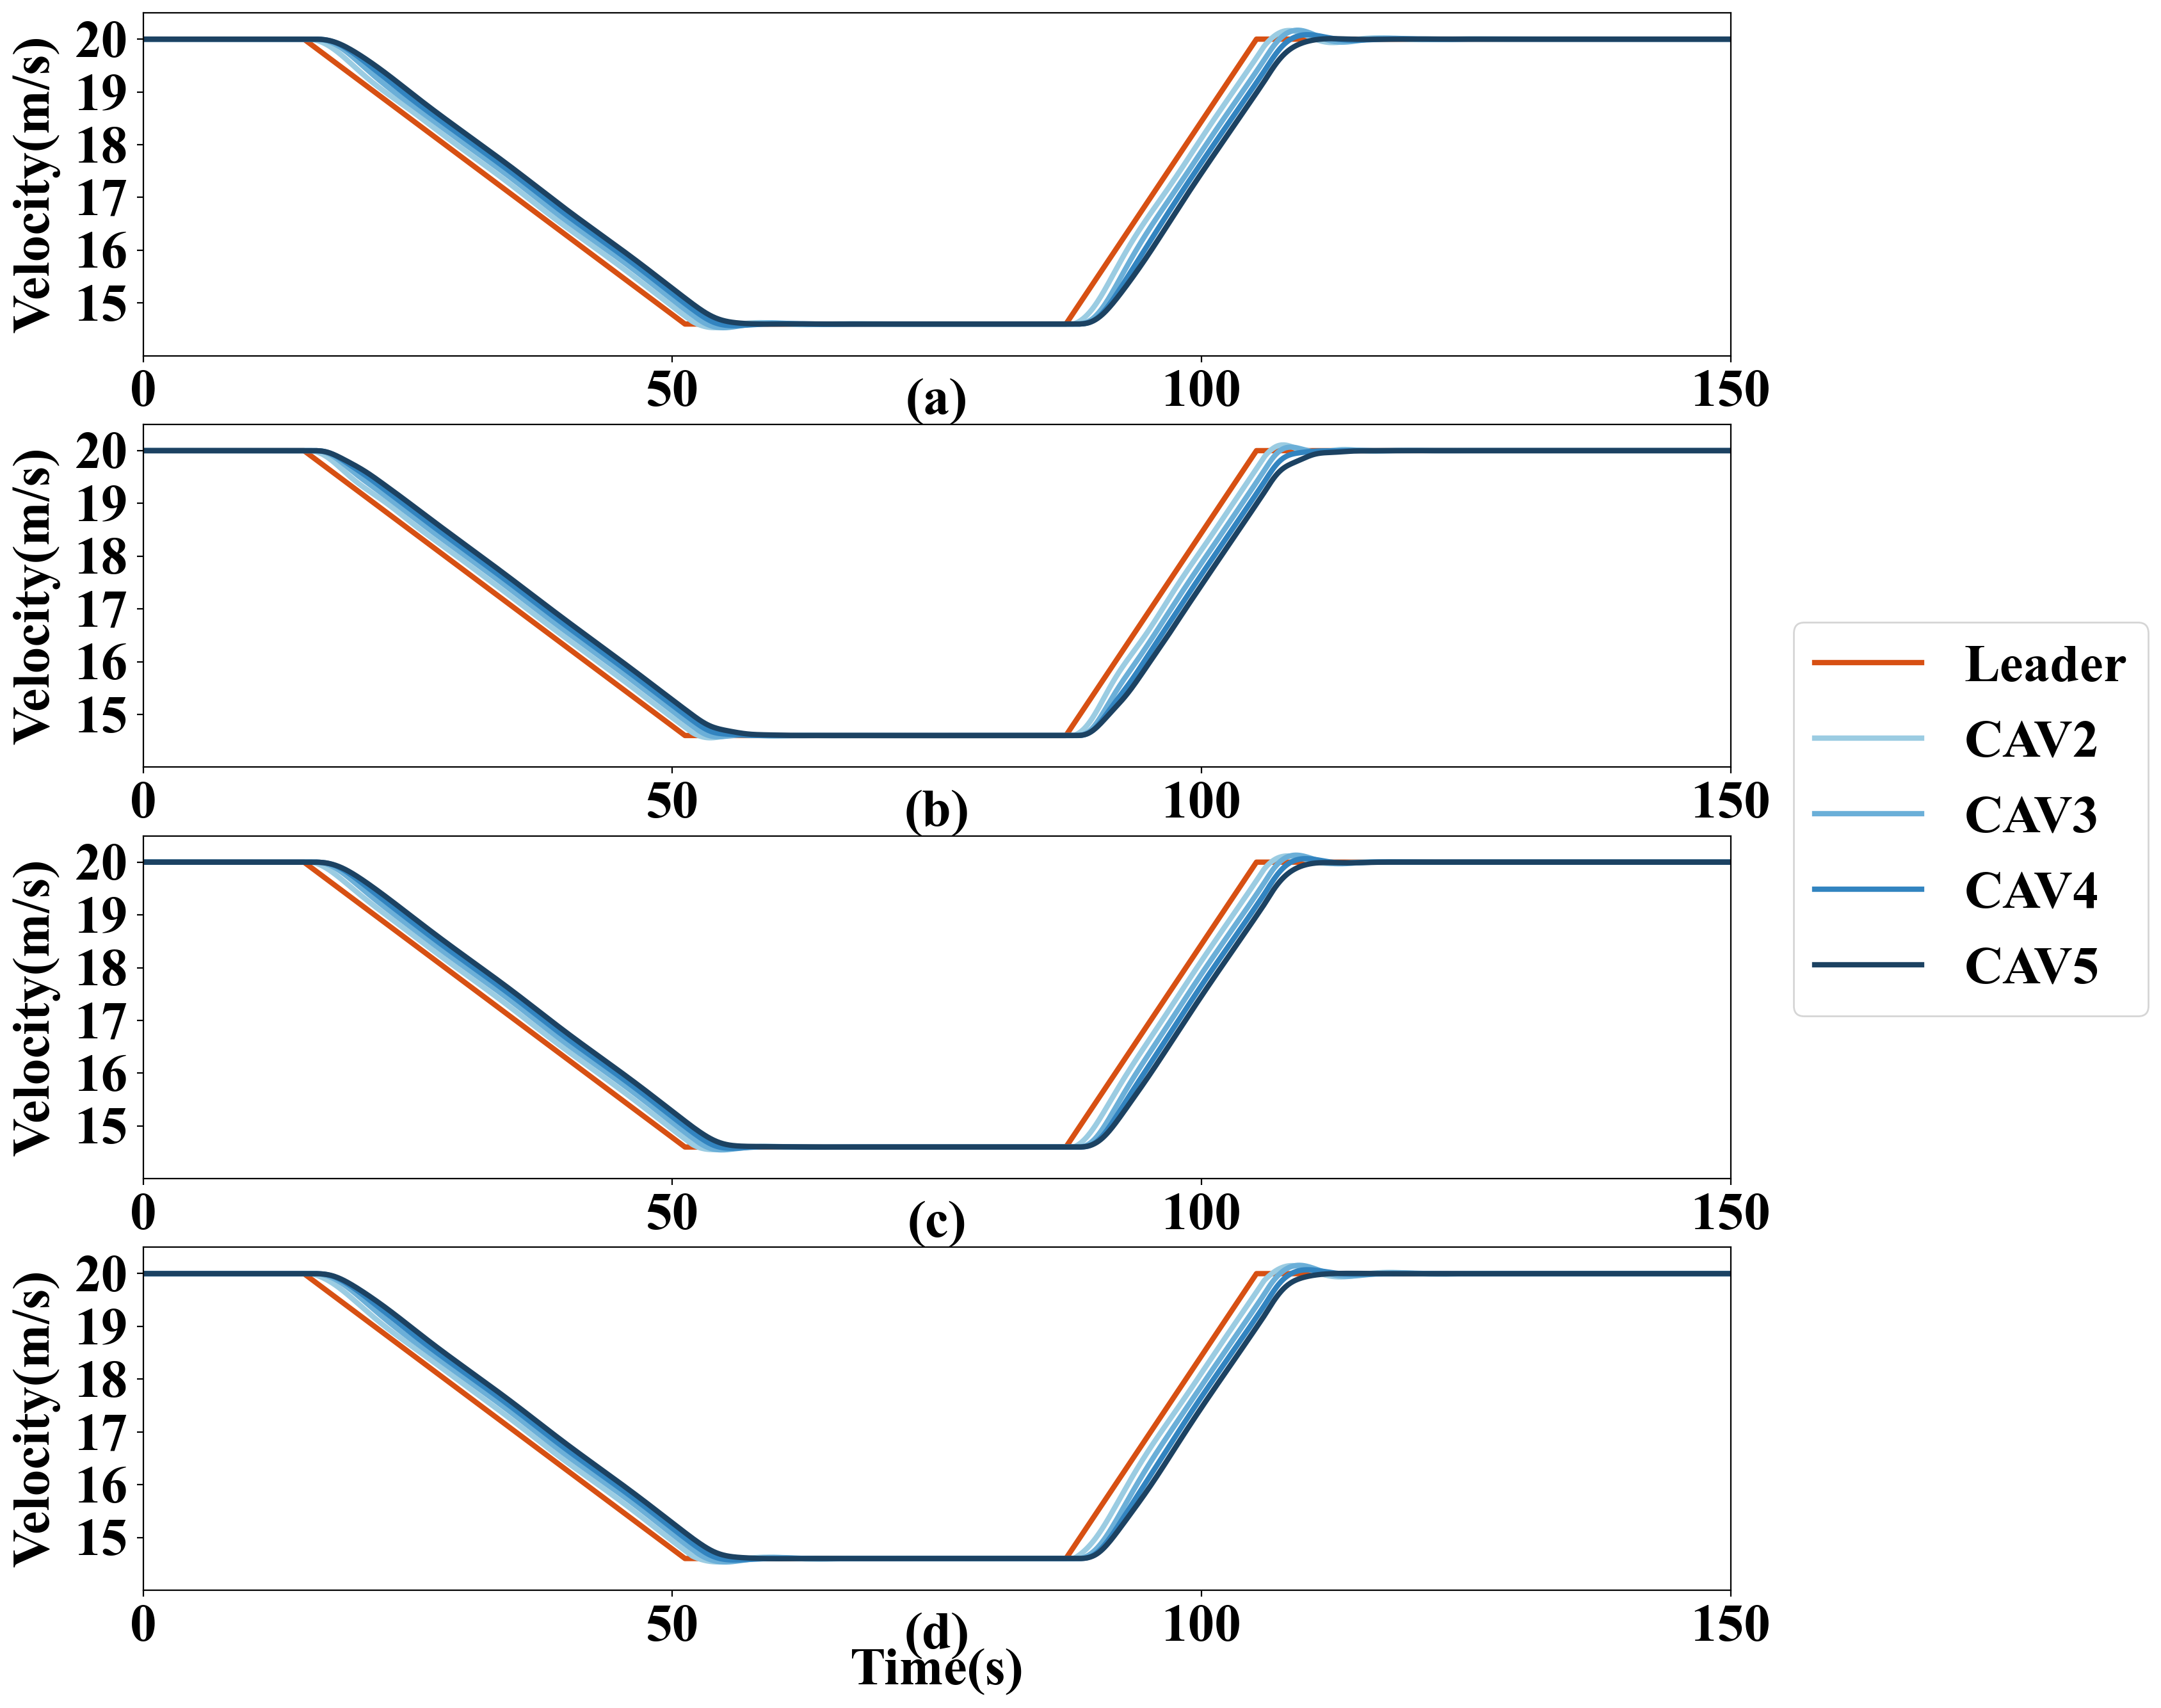
\includegraphics[width=8.5cm]{figs/fig9.png}
  \caption{~String stability's surface depending on YK $\gamma_{acc}$ and $\gamma_{cacc}$.}
  \label{fig9}
\end{figure}
We can conclude from Fig.~\ref{fig9} that the intersection of the transparent plane and string stability's surface is the basis for selecting $\gamma_{acc}$ and $\gamma_{cacc}$, which can ensure string stability and tap the advantages of CACPC as much as possible. However, the above margin stability curve can not be expressed explicitly analytically. Therefore, by the curve fitting method, we can get the expression of the intersection as follows (since any $\gamma$ can meet the string stability at platoon size = 5, there is no corresponding expression.):
\begin{equation}
  \gamma_{c a c c}= \begin{cases}-0.0501 * \gamma_{a c c}+0.2221 ,& \text { if } n=2 \\ -0.0248 * \gamma_{a c c}+0.5815 ,& \text { if } n=3 \\ -0.0165 * \gamma_{a c c}+0.8995 ,& \text { if } n=4\end{cases}.
\end{equation}
Moreover, with the help of the gain-scheduling method, the appropriate tuning function $\gamma$ that fits the margin stability curve is derived based on the expression above:
\begin{equation}
  \gamma_{a c c}=\left\{\begin{array}{cc}
    0 ,   & \text { if } n=1 \\
    0.4 , & \text { if } n=2 \\
    0.7 , & \text { if } n=3 \\
    0.9 , & \text { if } n=4 \\
    1 ,   & \text { if } n=5
  \end{array}\right.,
\end{equation}
\begin{equation}
  \gamma_{c a c c}=\left\{\begin{array}{cc}
    0 ,   & \text { if } n=1 \\
    0.3 , & \text { if } n=2 \\
    0.6 , & \text { if } n=3 \\
    0.9 , & \text { if } n=4 \\
    1 ,   & \text { if } n=5
  \end{array}\right.,
\end{equation}
where $n$ denotes platoon size.

\section{Numerical analyses}
\label{Section 5}

In this section, we first validate the string stability of CACPC based on the theoretical result derived in Section.~\ref{Section 4} by numerical simulation. Then a series of simulation experiments are conducted to explore the impact of YK parameterization on dynamic performance.

\subsection{Validation of string stability}
\label{Section 5.1}

\begin{figure}
  \centering
  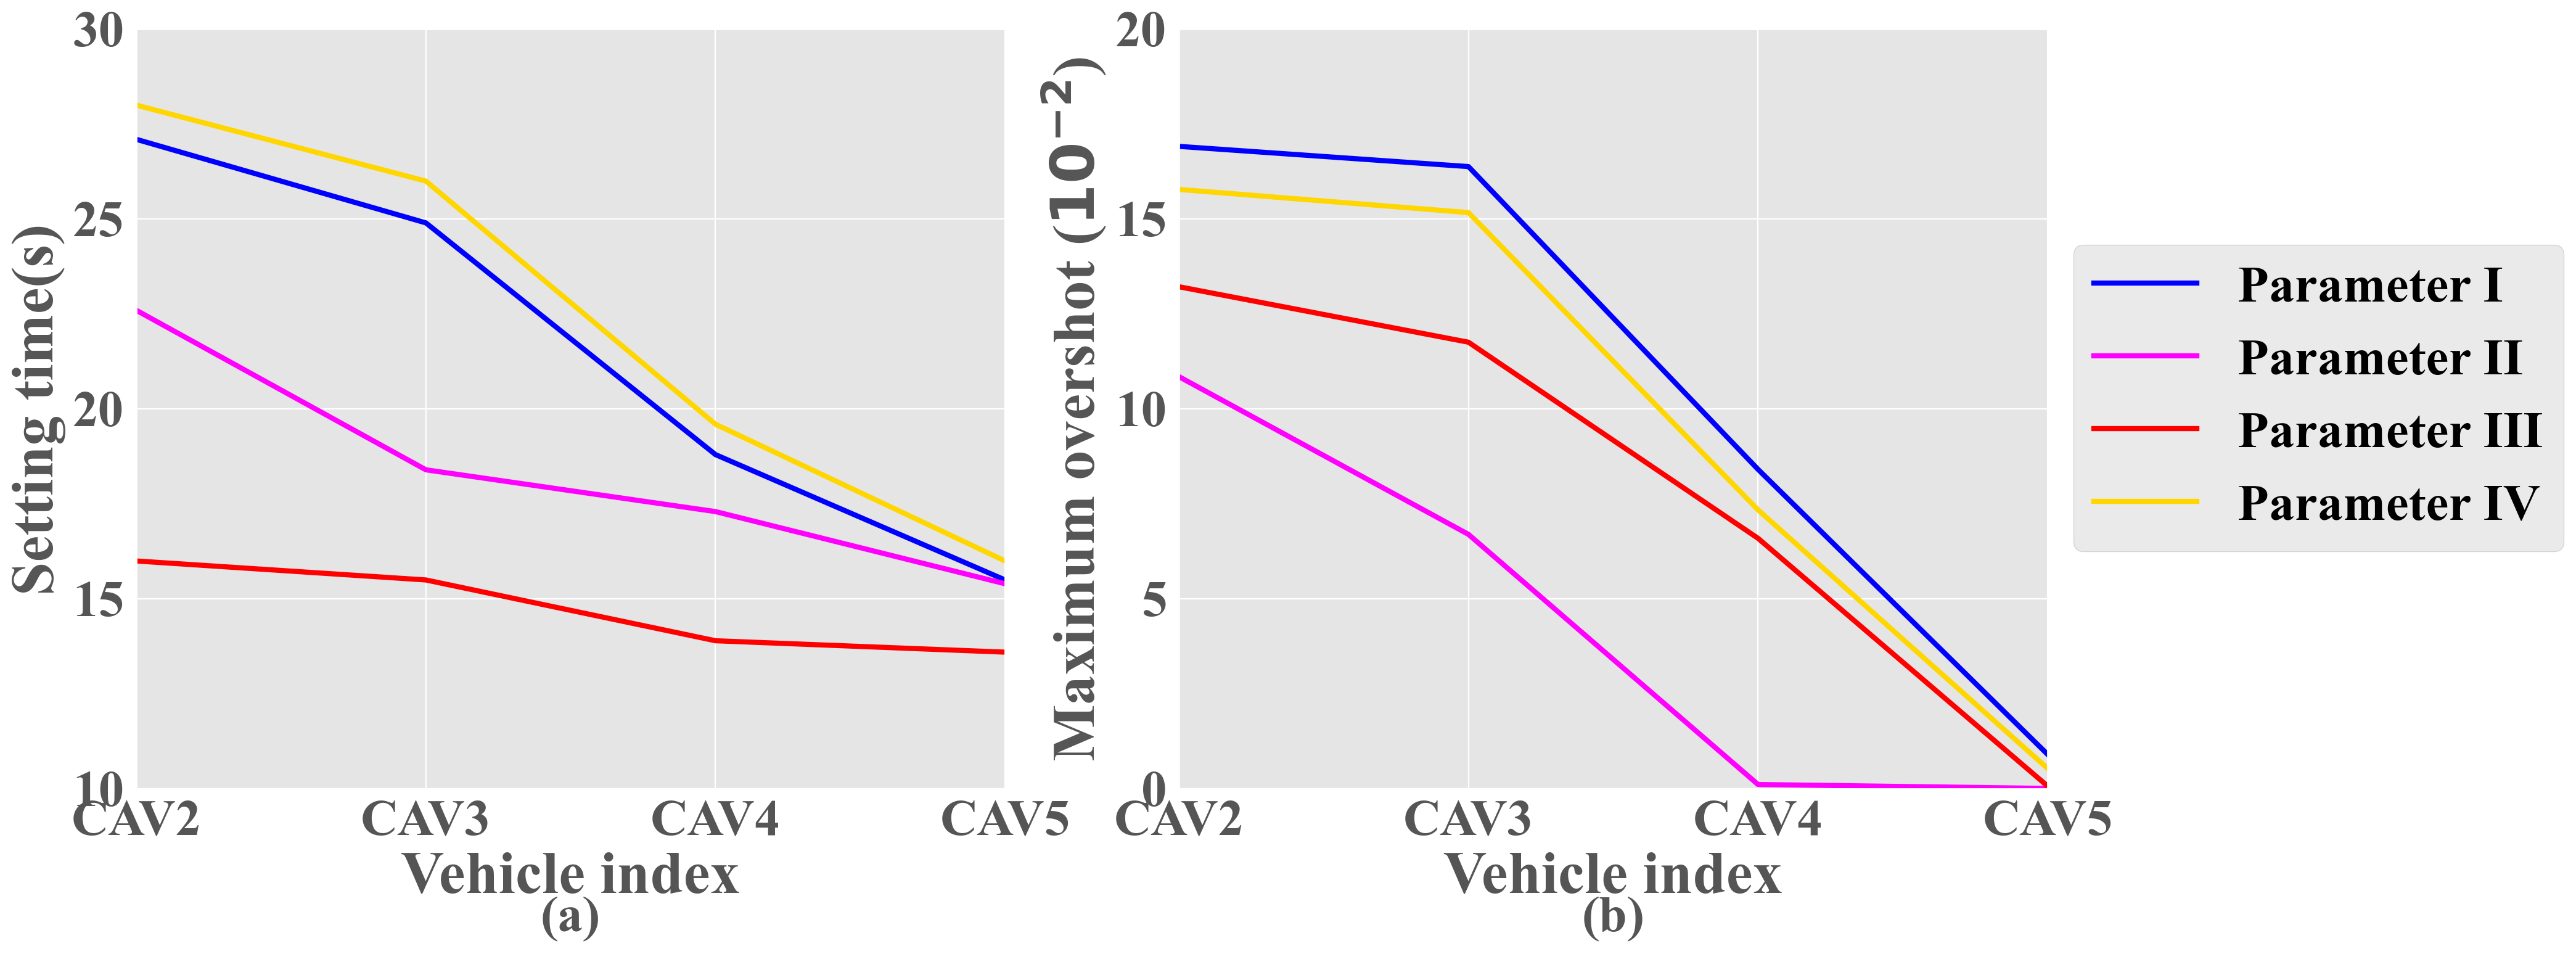
\includegraphics[width=8.5cm]{figs/fig10.png}
  \caption{~String stability's surface depends on platoon size.}
  \label{fig10}
\end{figure}

Based on the results in Section.~\ref{Section 4.2} and ~\ref{Section 4.3}, we have obtained the amplitude of CACPC under different platoon sizes. It is necessary to keep the string stable to prevent the perturbation from being amplified during propagation. Therefore, a numerical experiment is conducted to explore the string stability of the CACC platoon under low frequency ($10^{-5} - 10^0$ Hz). Fig.~\ref{fig10} shows the result where the curved surface represents the amplitude of the CACC platoon under low frequency ($10^{-5} - 10^0$ Hz) and different platoon sizes, and the bottom plane is the projection of the curved surface. Besides, the amplitude of the Y-axis is the amplification of the amplitude after the interference propagates through the CACC platoon, where amplitude $\le 1$ means that the CACC platoon is string stable; otherwise, it is string instable.

Fig.~\ref{fig10} shows that the string stability surface of the CACPC is below 1 for different frequencies and platoon sizes, indicating that the CACPC proposed above can avoid amplifying perturbation. Therefore, one conclusion can be drawn that the CACPC can ensure string stability under different platoon sizes.

\subsection{Simulation experiments of YK parameterization}
\label{Section 5.2}

Unlike theoretical analyses, behaviors observed in simulation experiments are closer to those in the real traffic environment. In order to further explore the actual effect of the controller switching using the YK parameterization, a series of simulation experiments are carried out based on CACPC as a supplement to the theoretical analysis. It should be noted that for the cases without YK parameterization, since there is no adaptive platoon size control strategy, the fixed platoon control strategy, i.e. it only functions when the platoon size reaches the specified platoon size.

\subsubsection{Simulation experiments maintain a constant speed during the forming and splitting process}
\label{Section 5.2.1}

~\\

\textit{Simulation scenario:} The simulation scenario is set as follows: at first, a leader vehicle drives on an infinitely long road under a given speed and acceleration configuration(containing five same small perturbations that occurred at the simulation time of 300s, 1000s, 1700s, 2400s, and 3100s under different platoon size). There are four experiments conducted:
\begin{enumerate}
  \item \textit{Experiment \uppercase\expandafter{\romannumeral1}:} The forming process of the CACC platoon with YK parameterization where an ACC (which is a CACC but degraded to an ACC functionally) follows the leader at the beginning, and more CACCs join the CACC platoon one by one at the simulation time of 700s, 1400s, 2100s, and 2800s.
  \item \textit{Experiment \uppercase\expandafter{\romannumeral2}:} The forming process of the CACC platoon without YK parameterization where an ACC (which is a CACC but degraded to an ACC functionally) follows the leader at the beginning, and more CACCs join the CACC platoon one by one at the simulation time of 700s, 1400s, 2100s, and 2800s. Note that since the fixed platoon control only functions when the platoon size reaches 5, the platoon control without YK parameterization is enabled after 2800s.
  \item \textit{Experiment \uppercase\expandafter{\romannumeral3}:} The splitting process of the CACC platoon with YK parameterization where an ACC (which is a CACC but degraded to an ACC functionally) and four CACCs follow the leader at the beginning, and the last CACC in the platoon leaves one by one at the simulation time of 700s, 1400s, 2100s, and 2800s.
  \item \textit{Experiment \uppercase\expandafter{\romannumeral4}:} The splitting process of the CACC platoon without YK parameterization where an ACC (which is a CACC but degraded to an ACC functionally) and four CACCs follow the leader at the beginning, and the last CACC in the platoon leaves one by one at the simulation time of 700s, 1400s, 2100s, and 2800s. Note that since the fixed platoon control only functions when the platoon size reaches 5, the platoon control without YK parameterization is enabled before 700s.
\end{enumerate}
The first pair of experiments is the forming process of the CACC platoon, where an ACC (which is a CACC but degraded to an ACC functionally) follows the leader at the beginning, and more CACCs join the CACC platoon one by one at the simulation time of 700s, 1400s, 2100s, and 2800s. Moreover, periodic perturbations are applied to the leader to explore the string stability of the CACC platoon under different platoon sizes. Another pair of experiments are conducted, simulating the splitting process of the CACC platoon. It should be noted that there are four experiments conducted to analyze the impact of the YK parameterization under the platoon forming case and the platoon splitting case. Experiment \uppercase\expandafter{\romannumeral1} and \uppercase\expandafter{\romannumeral3} applies YK parameterization with the tuning function $\gamma$ proposed above, while experiment \uppercase\expandafter{\romannumeral2} and \uppercase\expandafter{\romannumeral4} switch to the platoon control mode directly only the platoon size reaches maximum platoon size $S=5$.

\begin{figure}
  \centering
  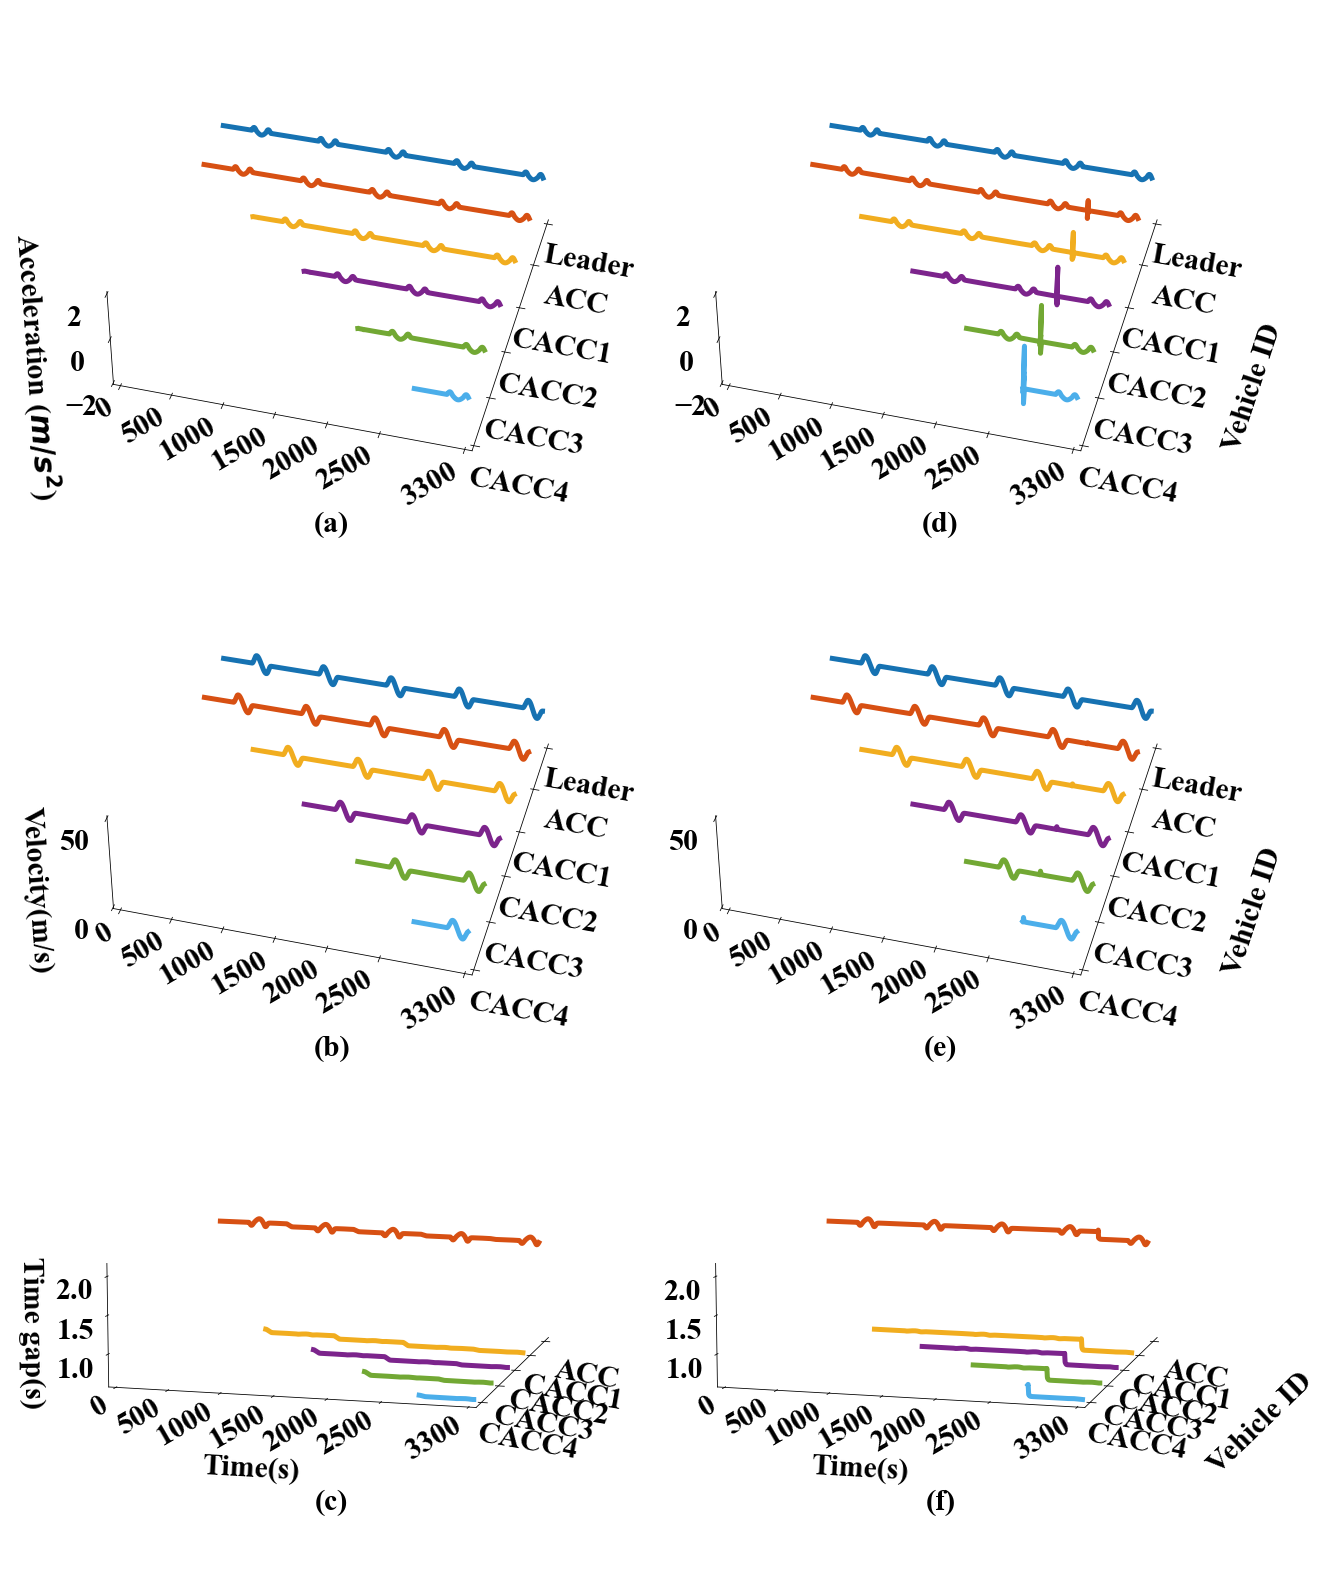
\includegraphics[width=8.5cm]{figs/c_form.png}
  \caption{~Simulation results of experiment \uppercase\expandafter{\romannumeral1} and \uppercase\expandafter{\romannumeral2}: CACPC with or without YK parameterization under the platoon forming case. (a)-(c) show the simulation results of experiment \uppercase\expandafter{\romannumeral1}, and (d)-(f) show the simulation results of experiment \uppercase\expandafter{\romannumeral2}. (a),(d) Acceleration of simulation results; (b),(e) Velocity of simulation results; (c),(f) Time gap of simulation results.}
  \label{new1}
\end{figure}

\begin{figure}
  \centering
  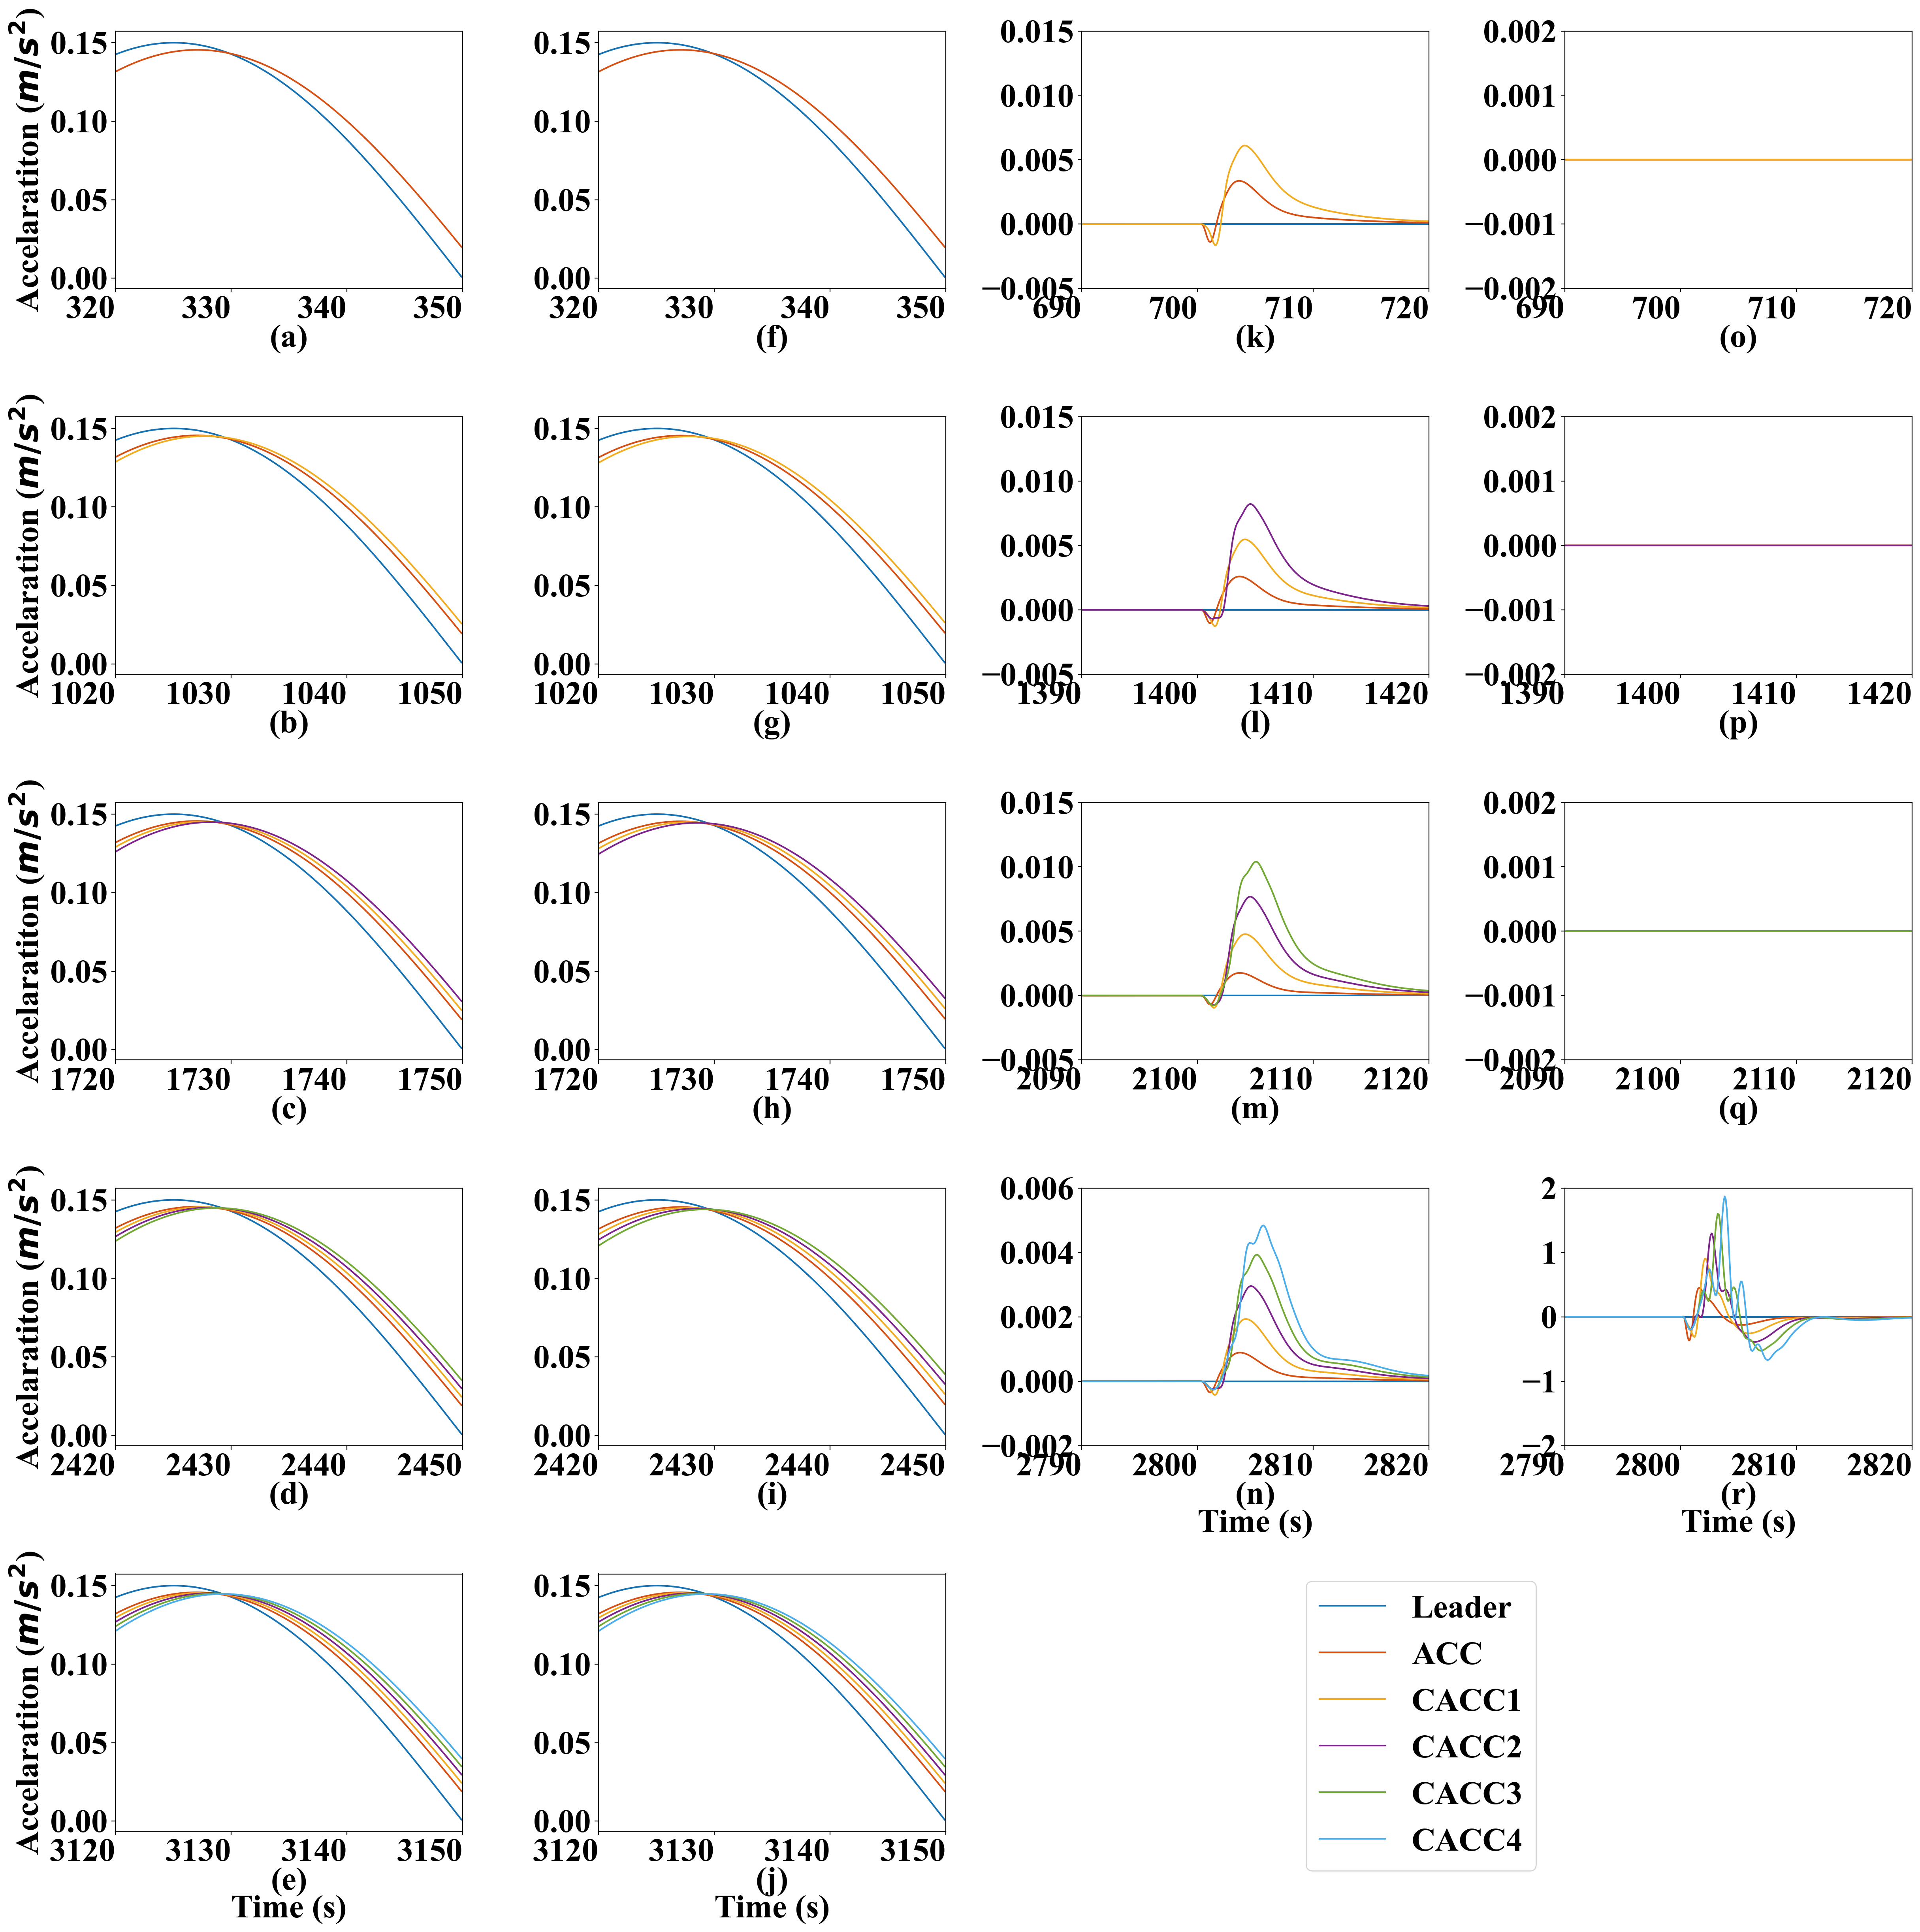
\includegraphics[width=8.5cm]{figs/form_detail.png}
  \caption{~Detailed perturbation simulation results of experiments \uppercase\expandafter{\romannumeral1} and \uppercase\expandafter{\romannumeral2}: CACPC with or without YK parameterization under the platoon forming case. For experiment \uppercase\expandafter{\romannumeral1}, (a)-(e) show the propagating processes of five applied perturbations, and (k)-(n) show the four switching processes. For experiment \uppercase\expandafter{\romannumeral2}, (f)-(j) show the propagating processes of five applied perturbations, and (o)-(r) show the four switching processes.}
  \label{new2}
\end{figure}

\begin{figure}
  \centering
  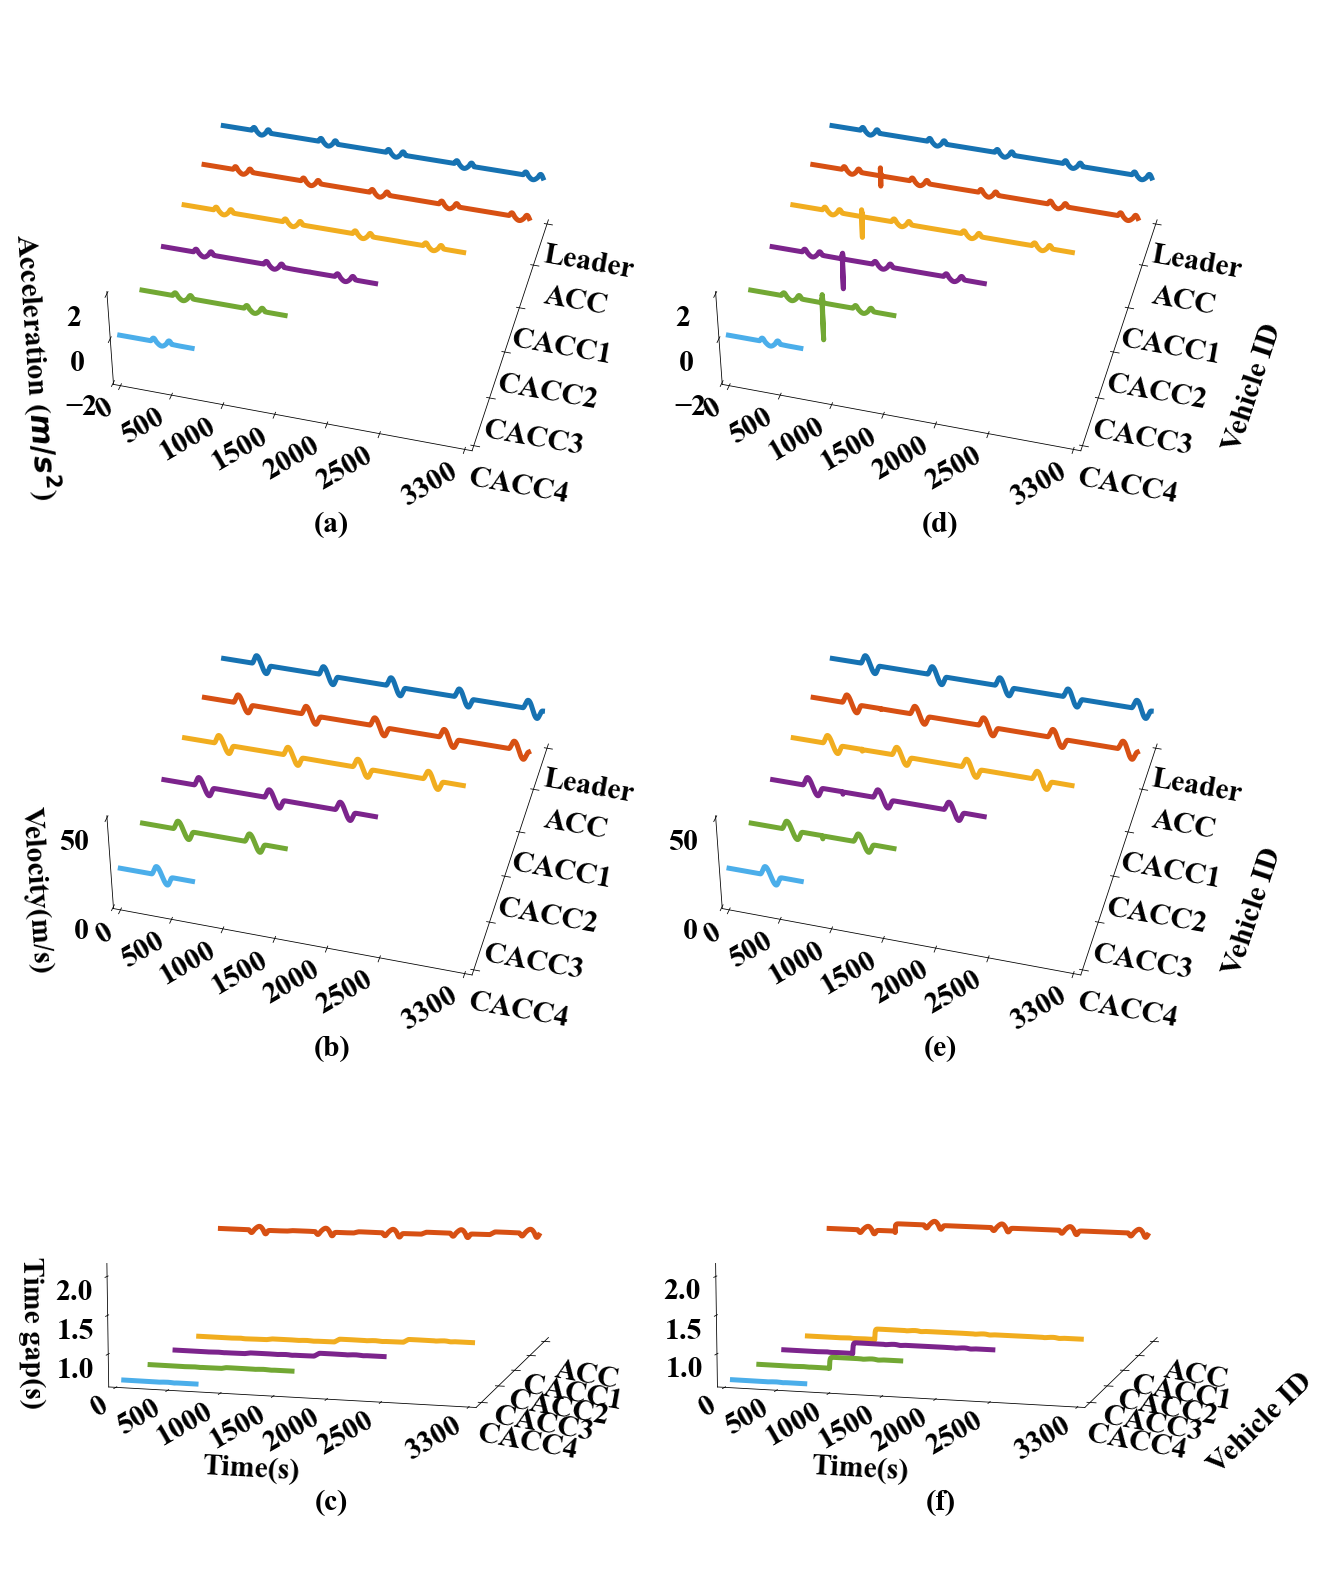
\includegraphics[width=8.5cm]{figs/c_split.png}
  \caption{~Simulation results of experiments \uppercase\expandafter{\romannumeral3} and \uppercase\expandafter{\romannumeral4}: CACPC with or without YK parameterization under the platoon splitting case. (a)-(c) show the simulation results of experiment \uppercase\expandafter{\romannumeral3}, and (d)-(f) show the simulation results of experiment \uppercase\expandafter{\romannumeral4}. (a),(d) Acceleration of simulation results; (b),(e) Velocity of simulation results; (c),(f) Time gap of simulation results.}
  \label{new3}
\end{figure}

\begin{figure}
  \centering
  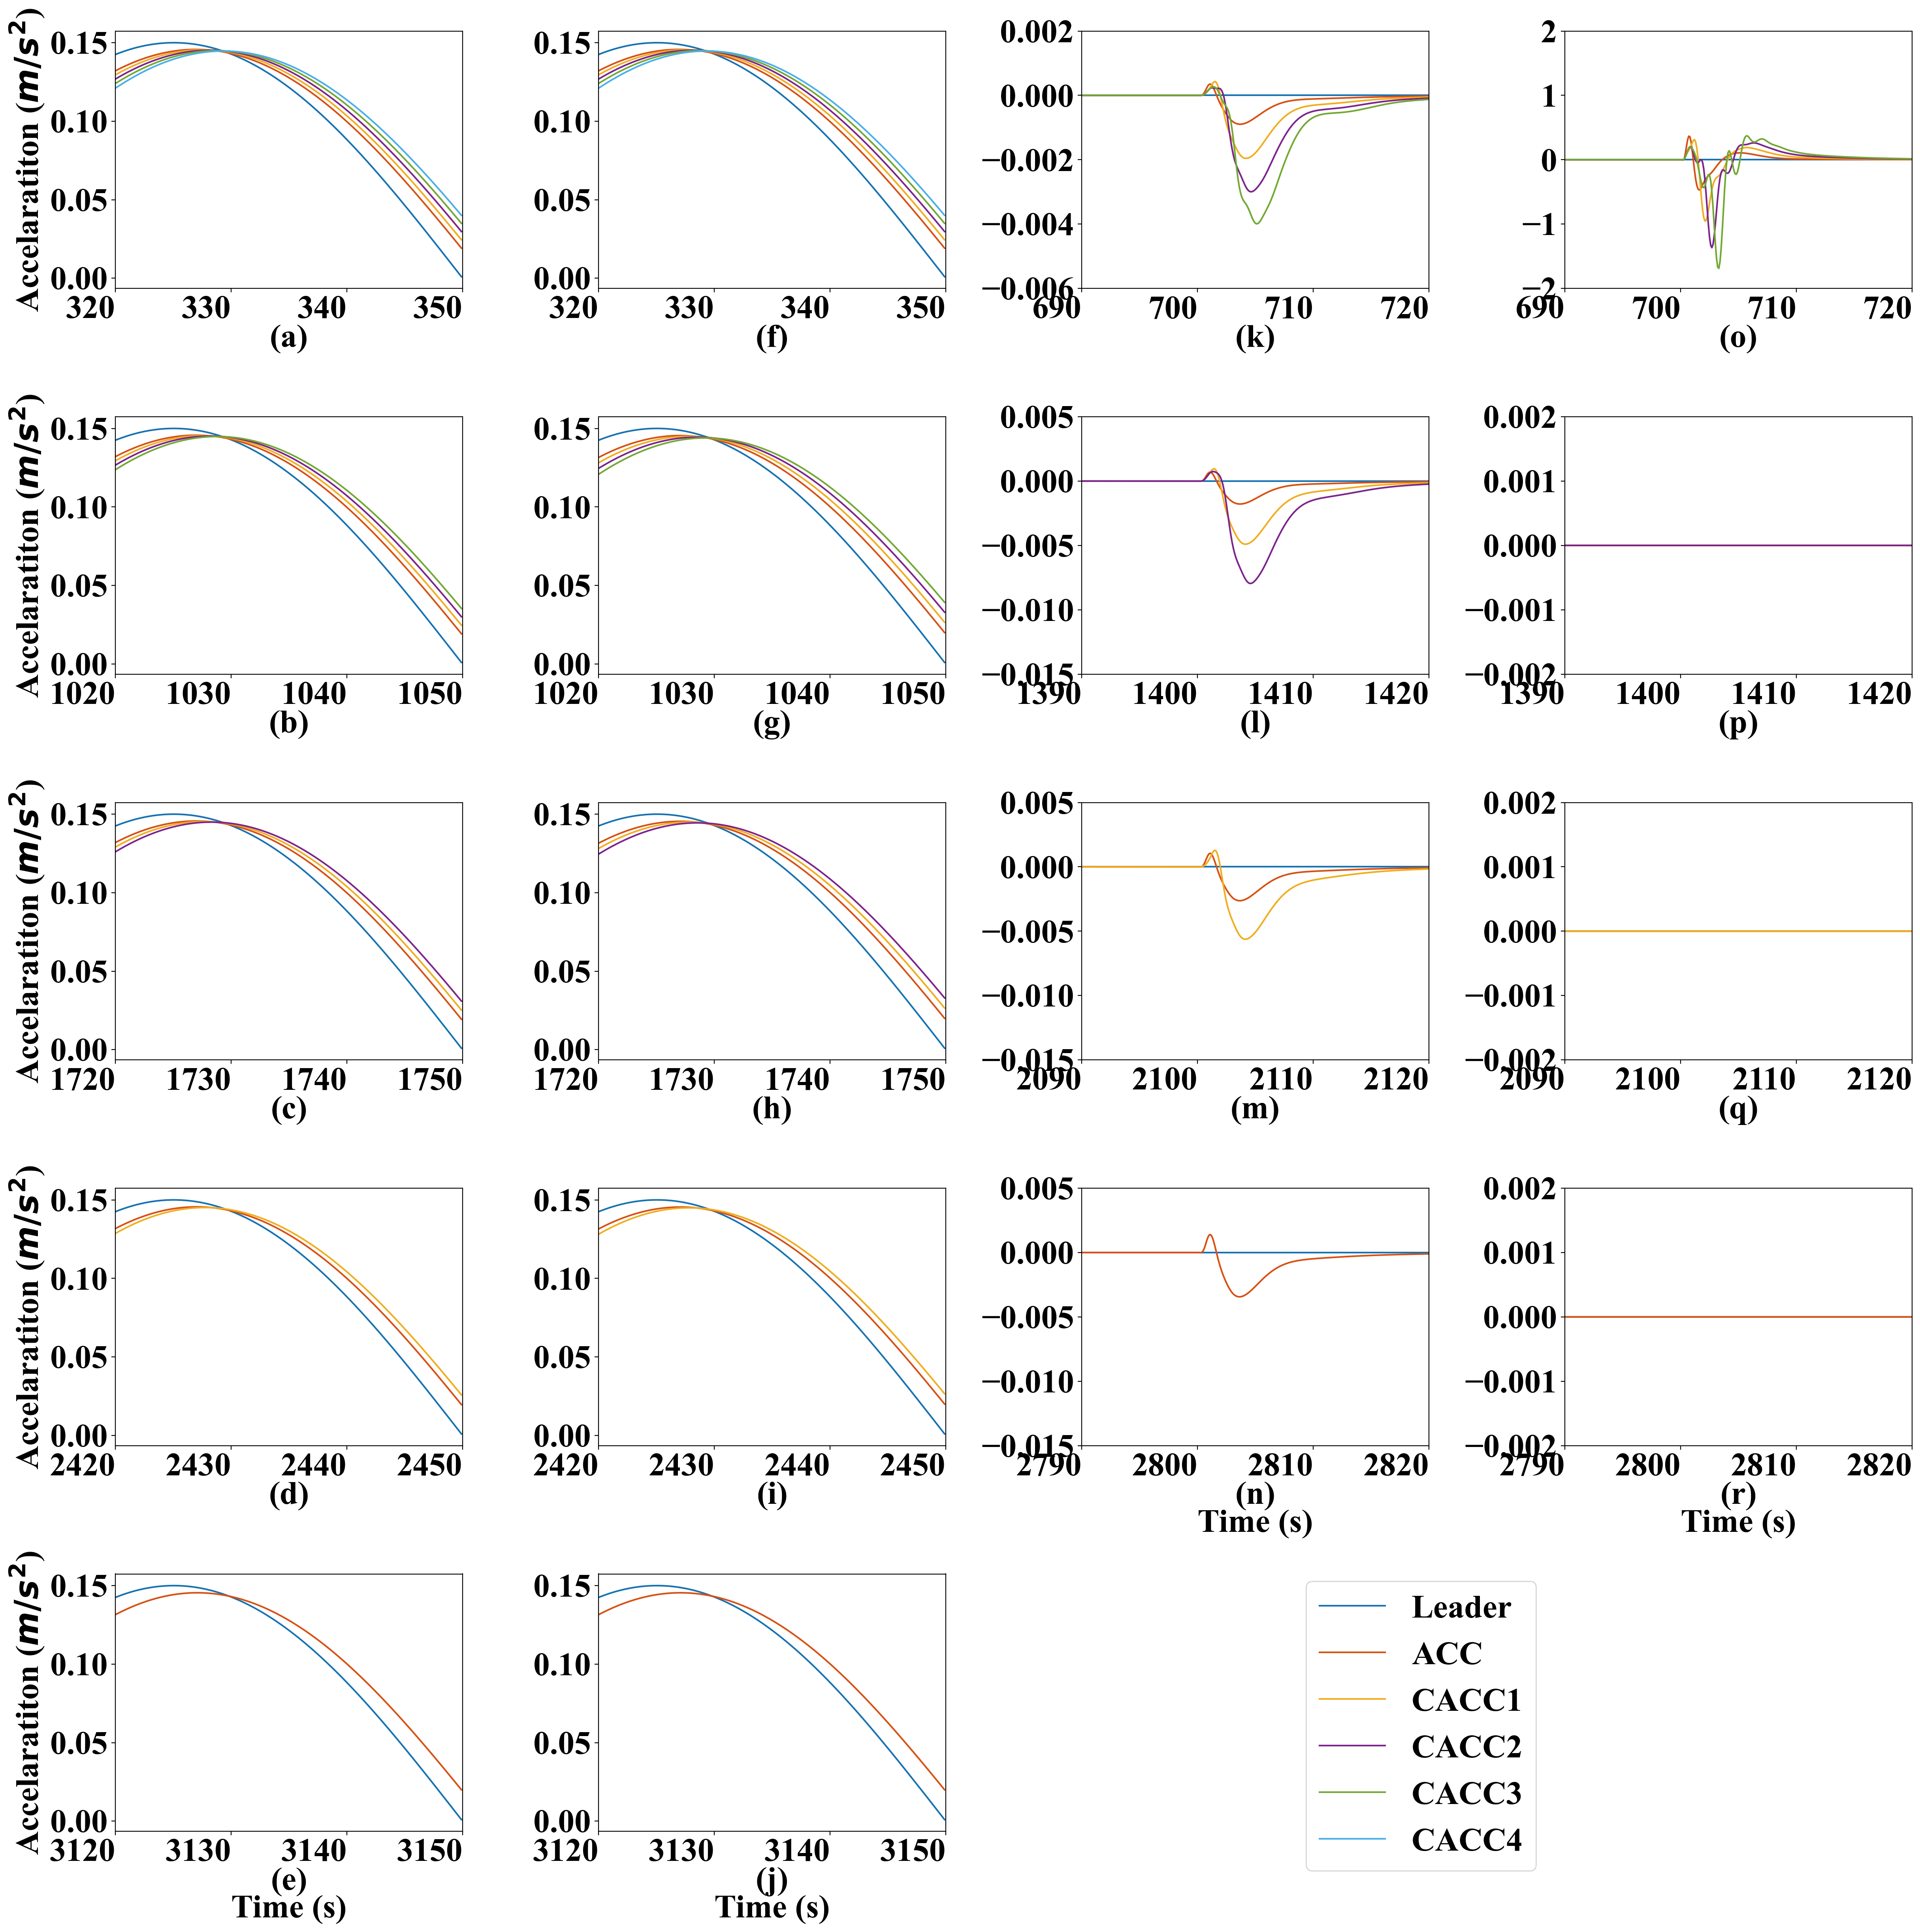
\includegraphics[width=8.5cm]{figs/split_detail.png}
  \caption{~Detailed perturbation simulation results of experiments \uppercase\expandafter{\romannumeral3} and \uppercase\expandafter{\romannumeral4}: CACPC with or without YK parameterization under the platoon splitting case. For experiment \uppercase\expandafter{\romannumeral3}, (a)-(e) show the propagating processes of five applied perturbations, and (k)-(n) show the four switching processes. For experiment \uppercase\expandafter{\romannumeral4}, (f)-(j) show the propagating processes of five applied perturbations, and (o)-(r) show the four switching processes.}
  \label{new4}
\end{figure}

% \begin{figure}
% 	\centering
% 		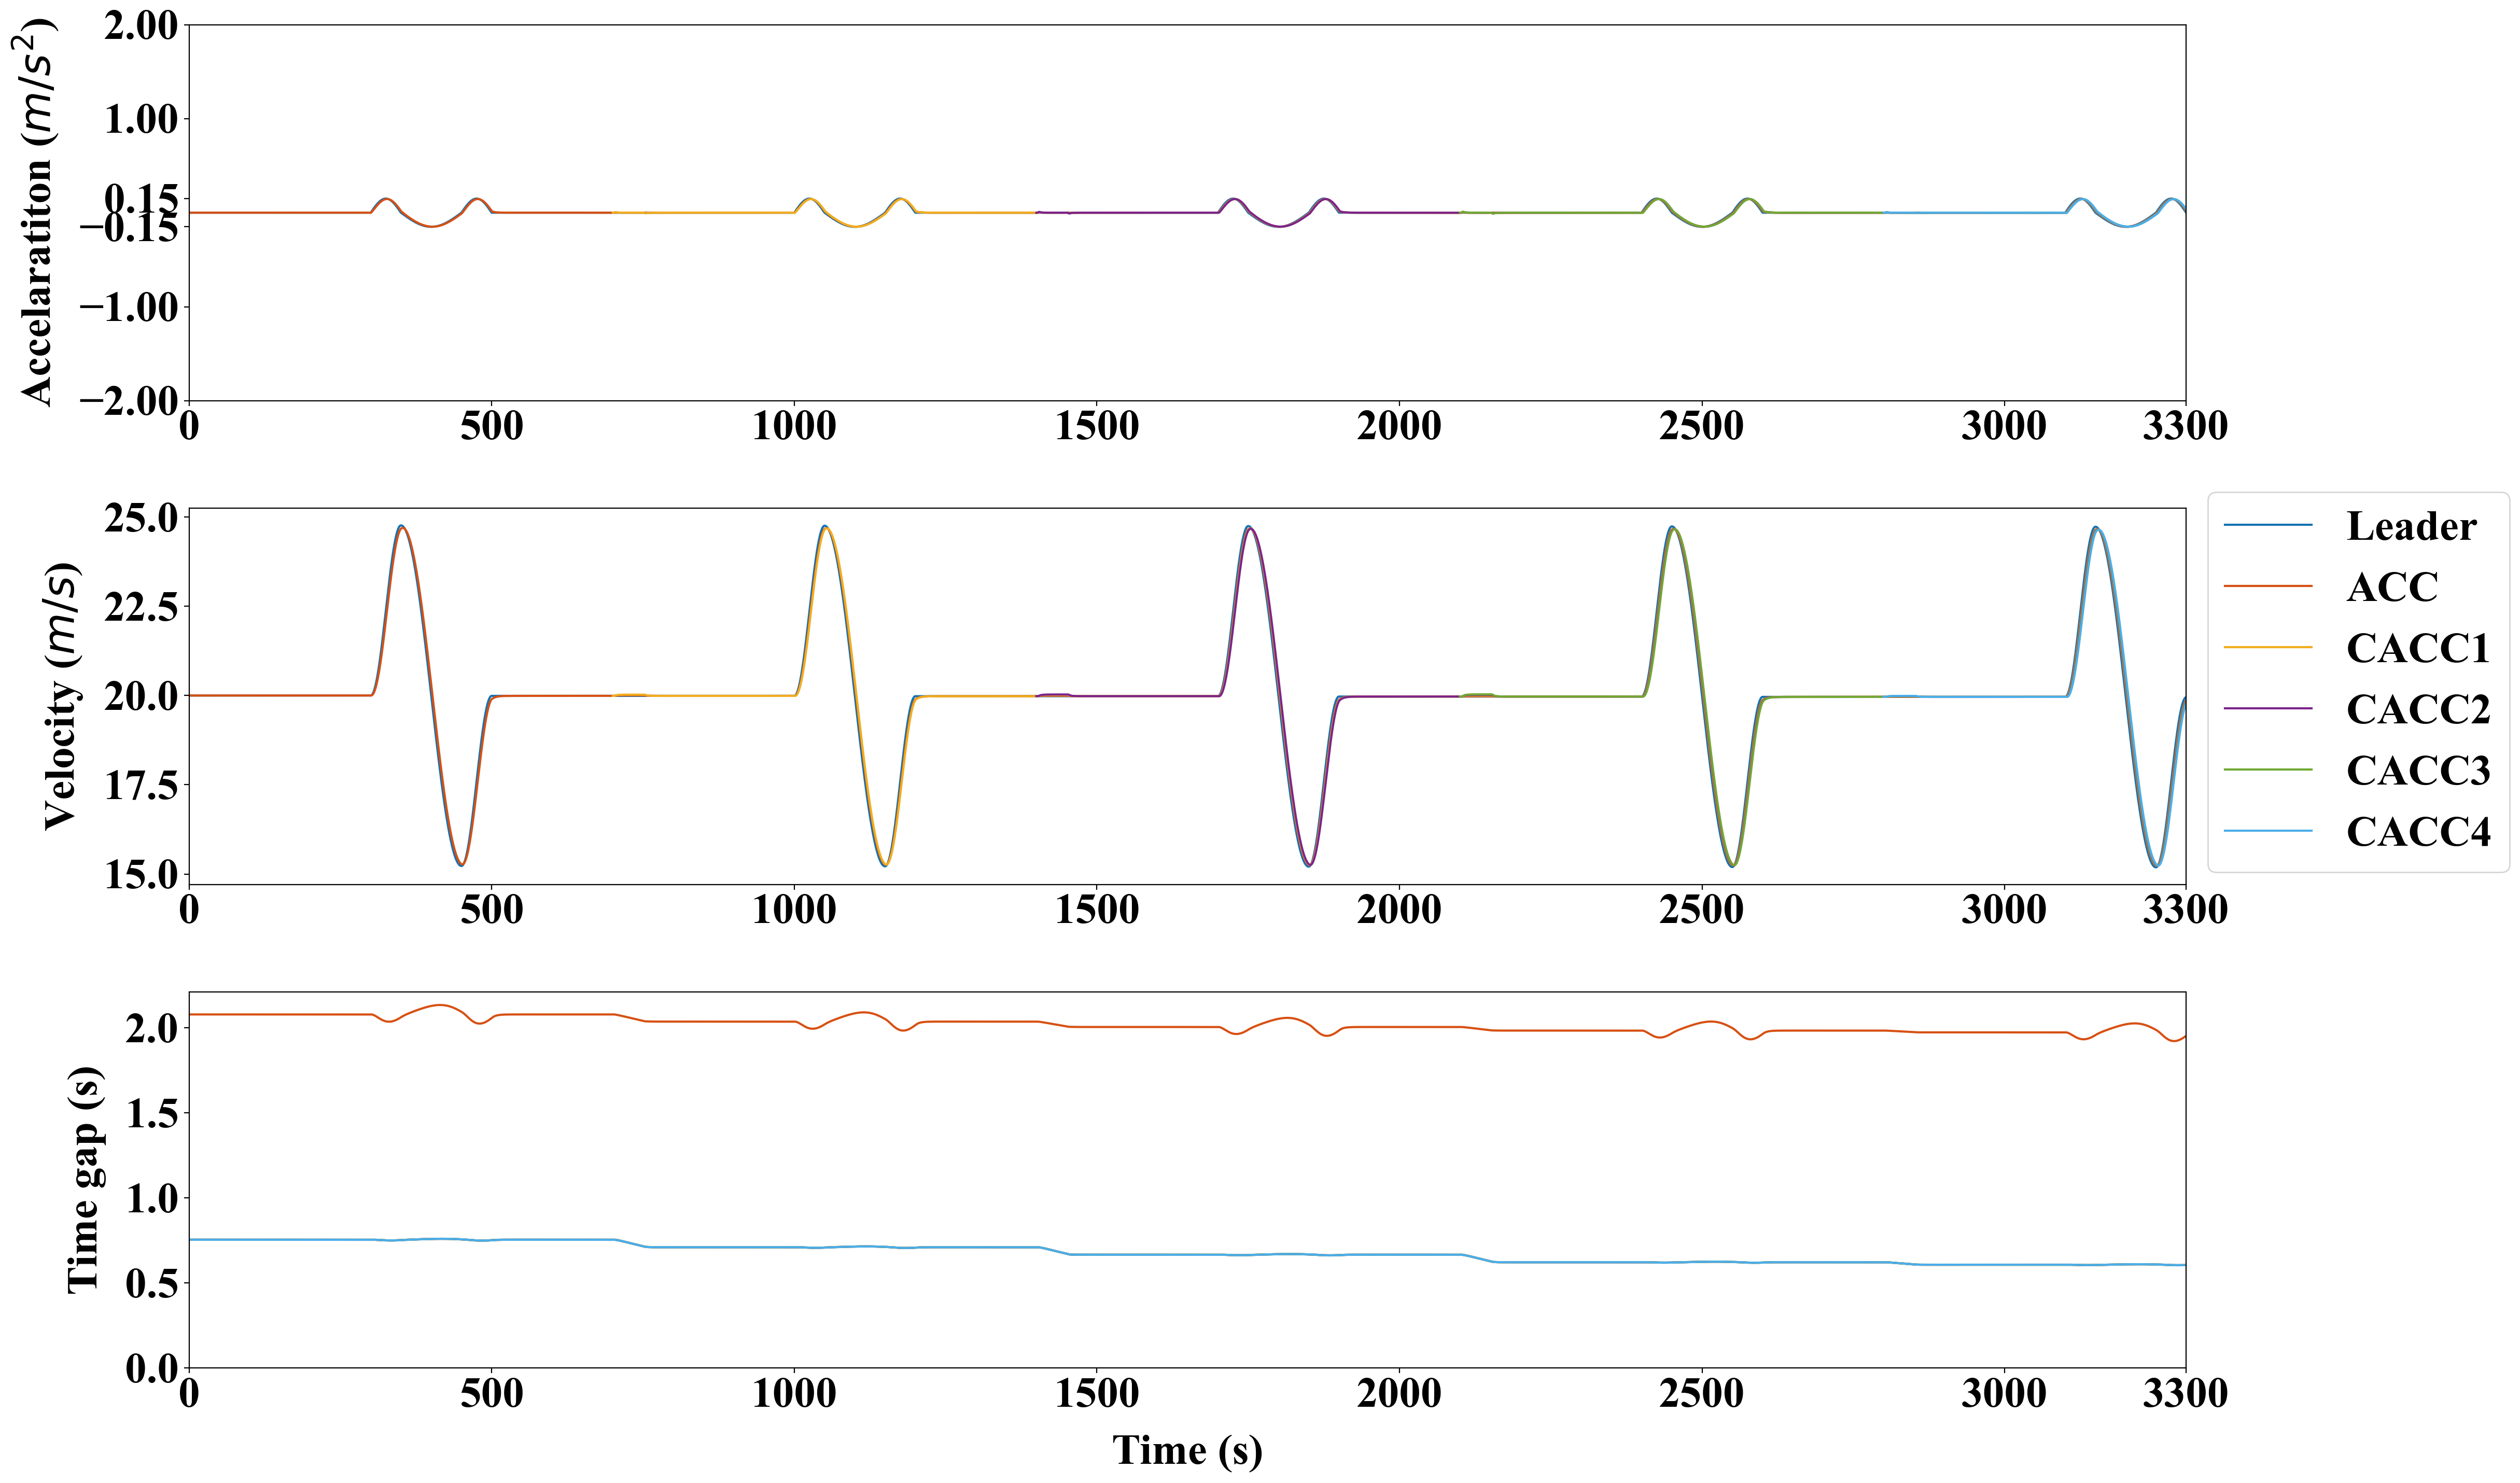
\includegraphics[width=14cm]{figs/fig11.png}
% 	\caption{Simulation results of experiment one: CACPC with YK parameterization under the platoon forming case.}
% 	\label{fig11}
% \end{figure}

% \begin{figure}
% 	\centering
% 		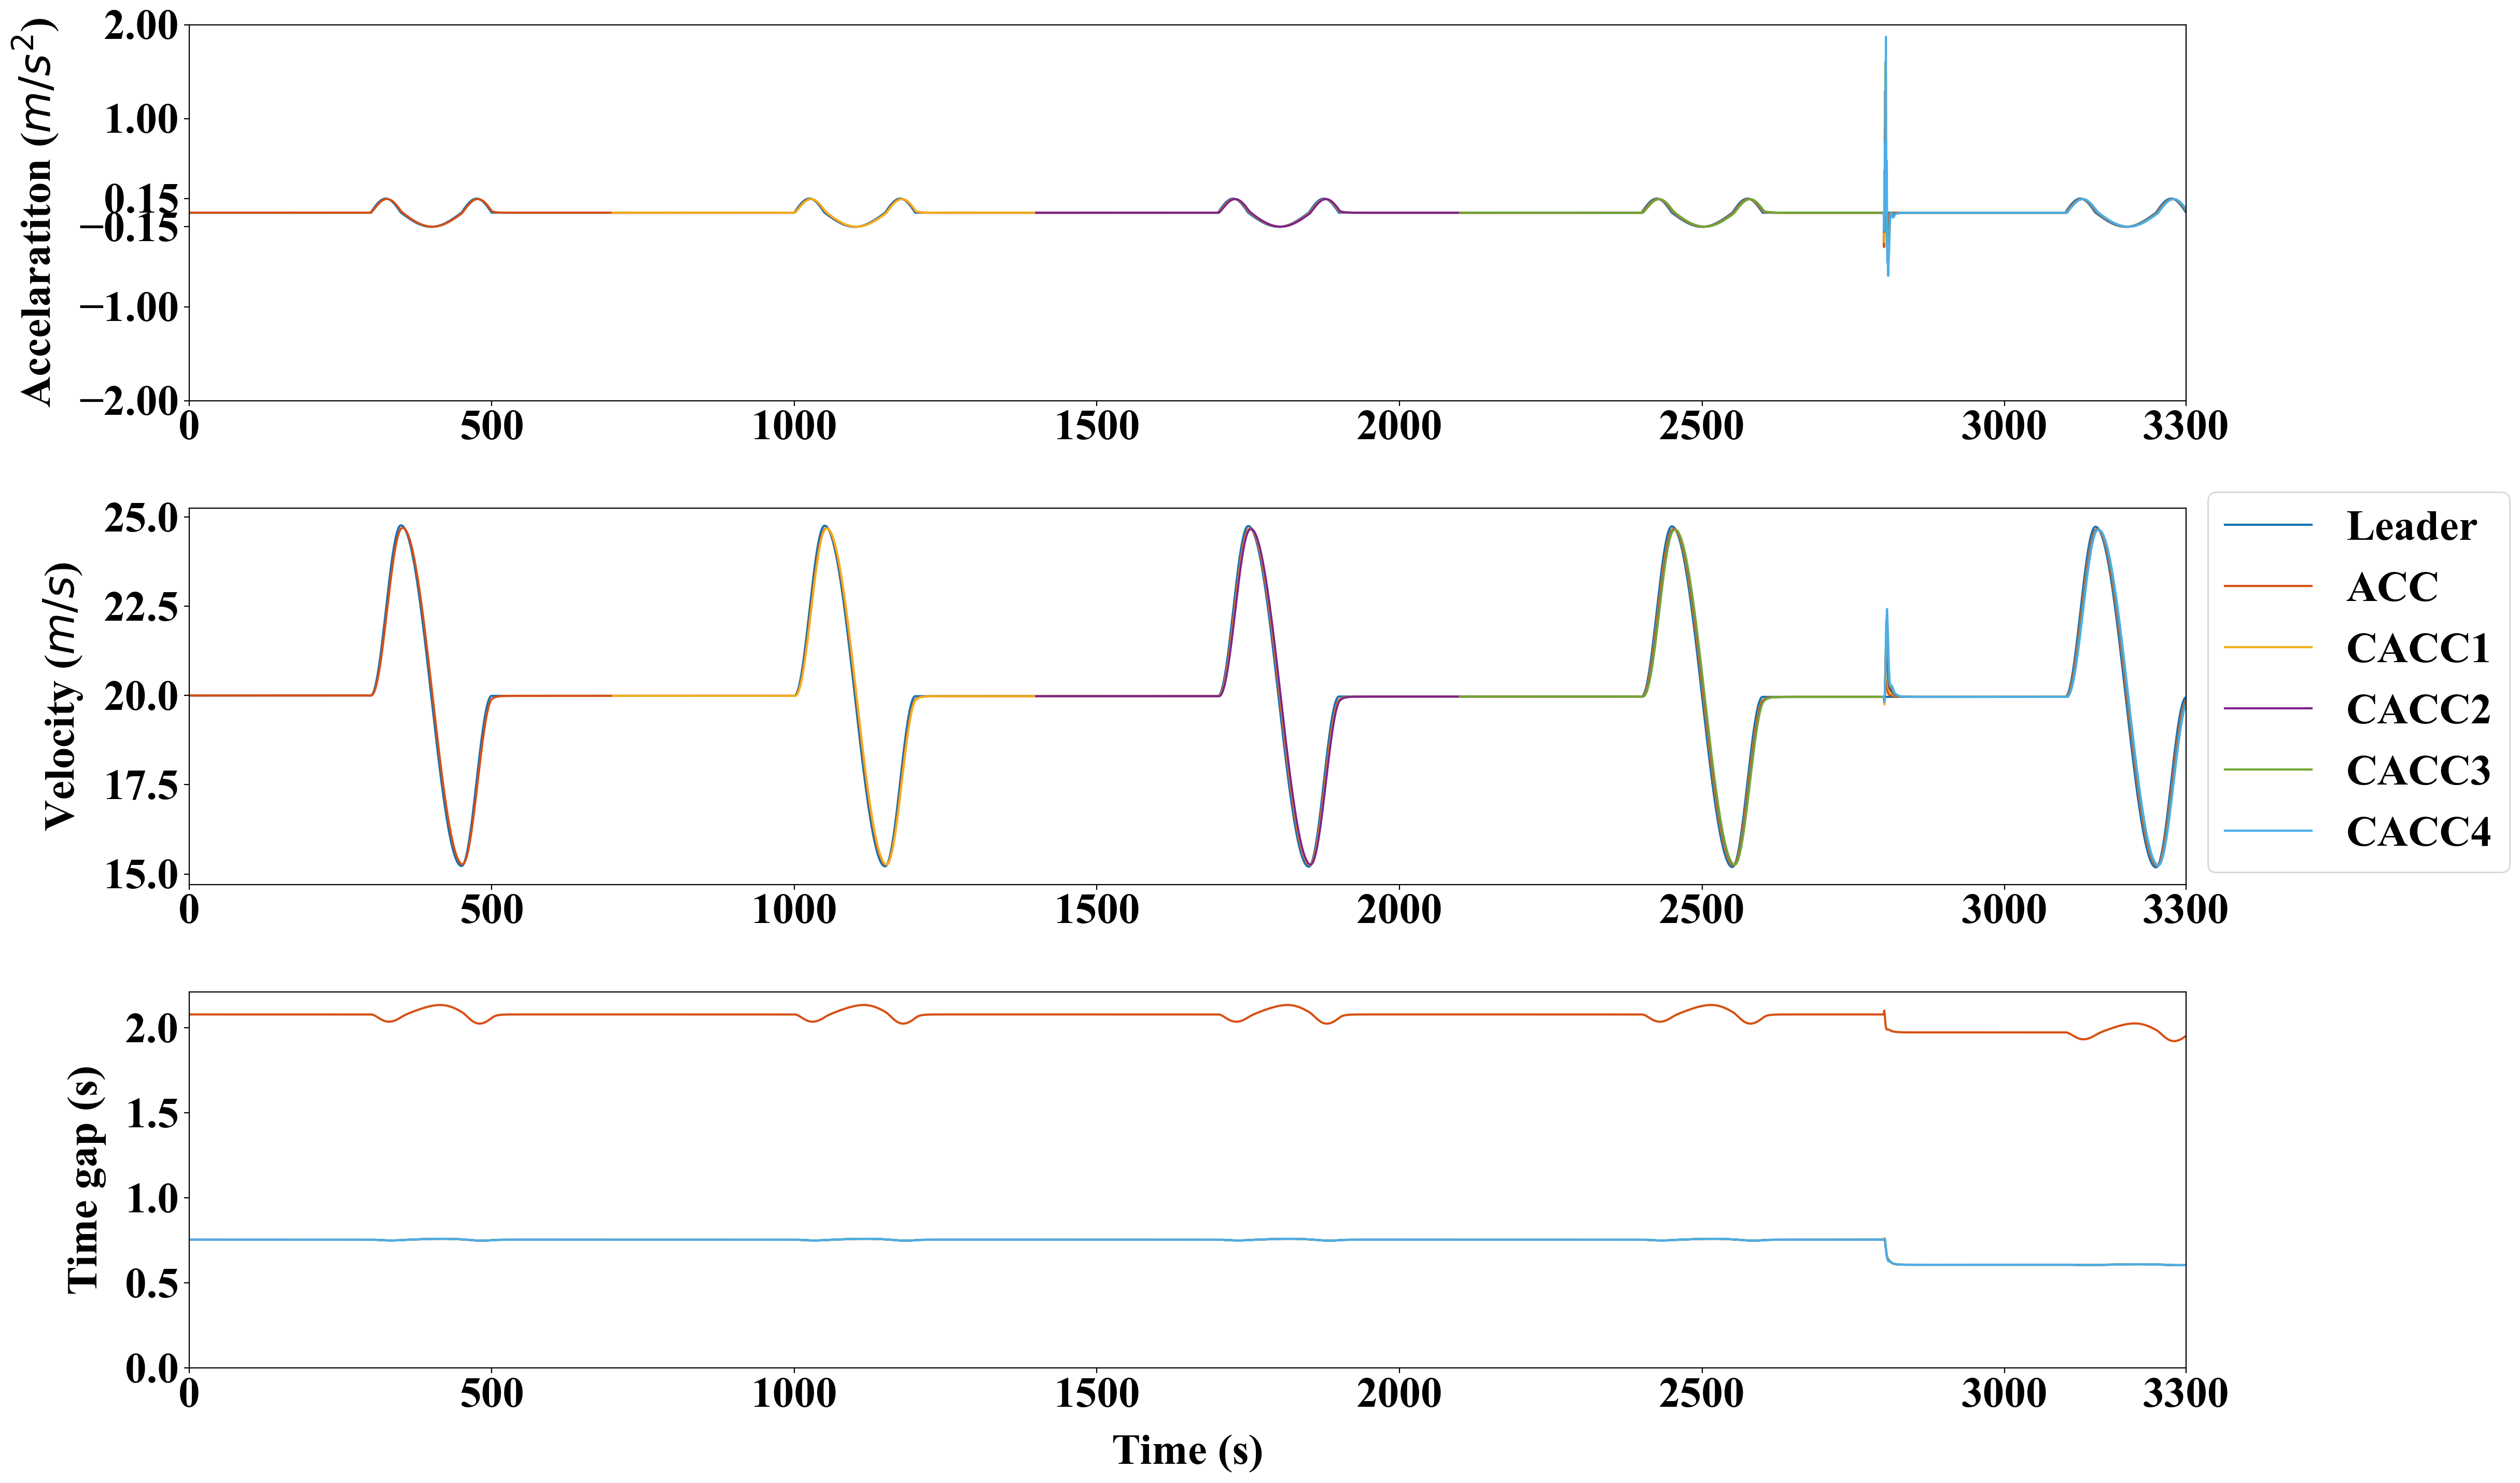
\includegraphics[width=14cm]{figs/fig12.png}
% 	\caption{Simulation results of experiment two: CACPC without YK parameterization under the platoon forming case.}
% 	\label{fig12}
% \end{figure}

% \begin{figure}
% 	\centering
% 		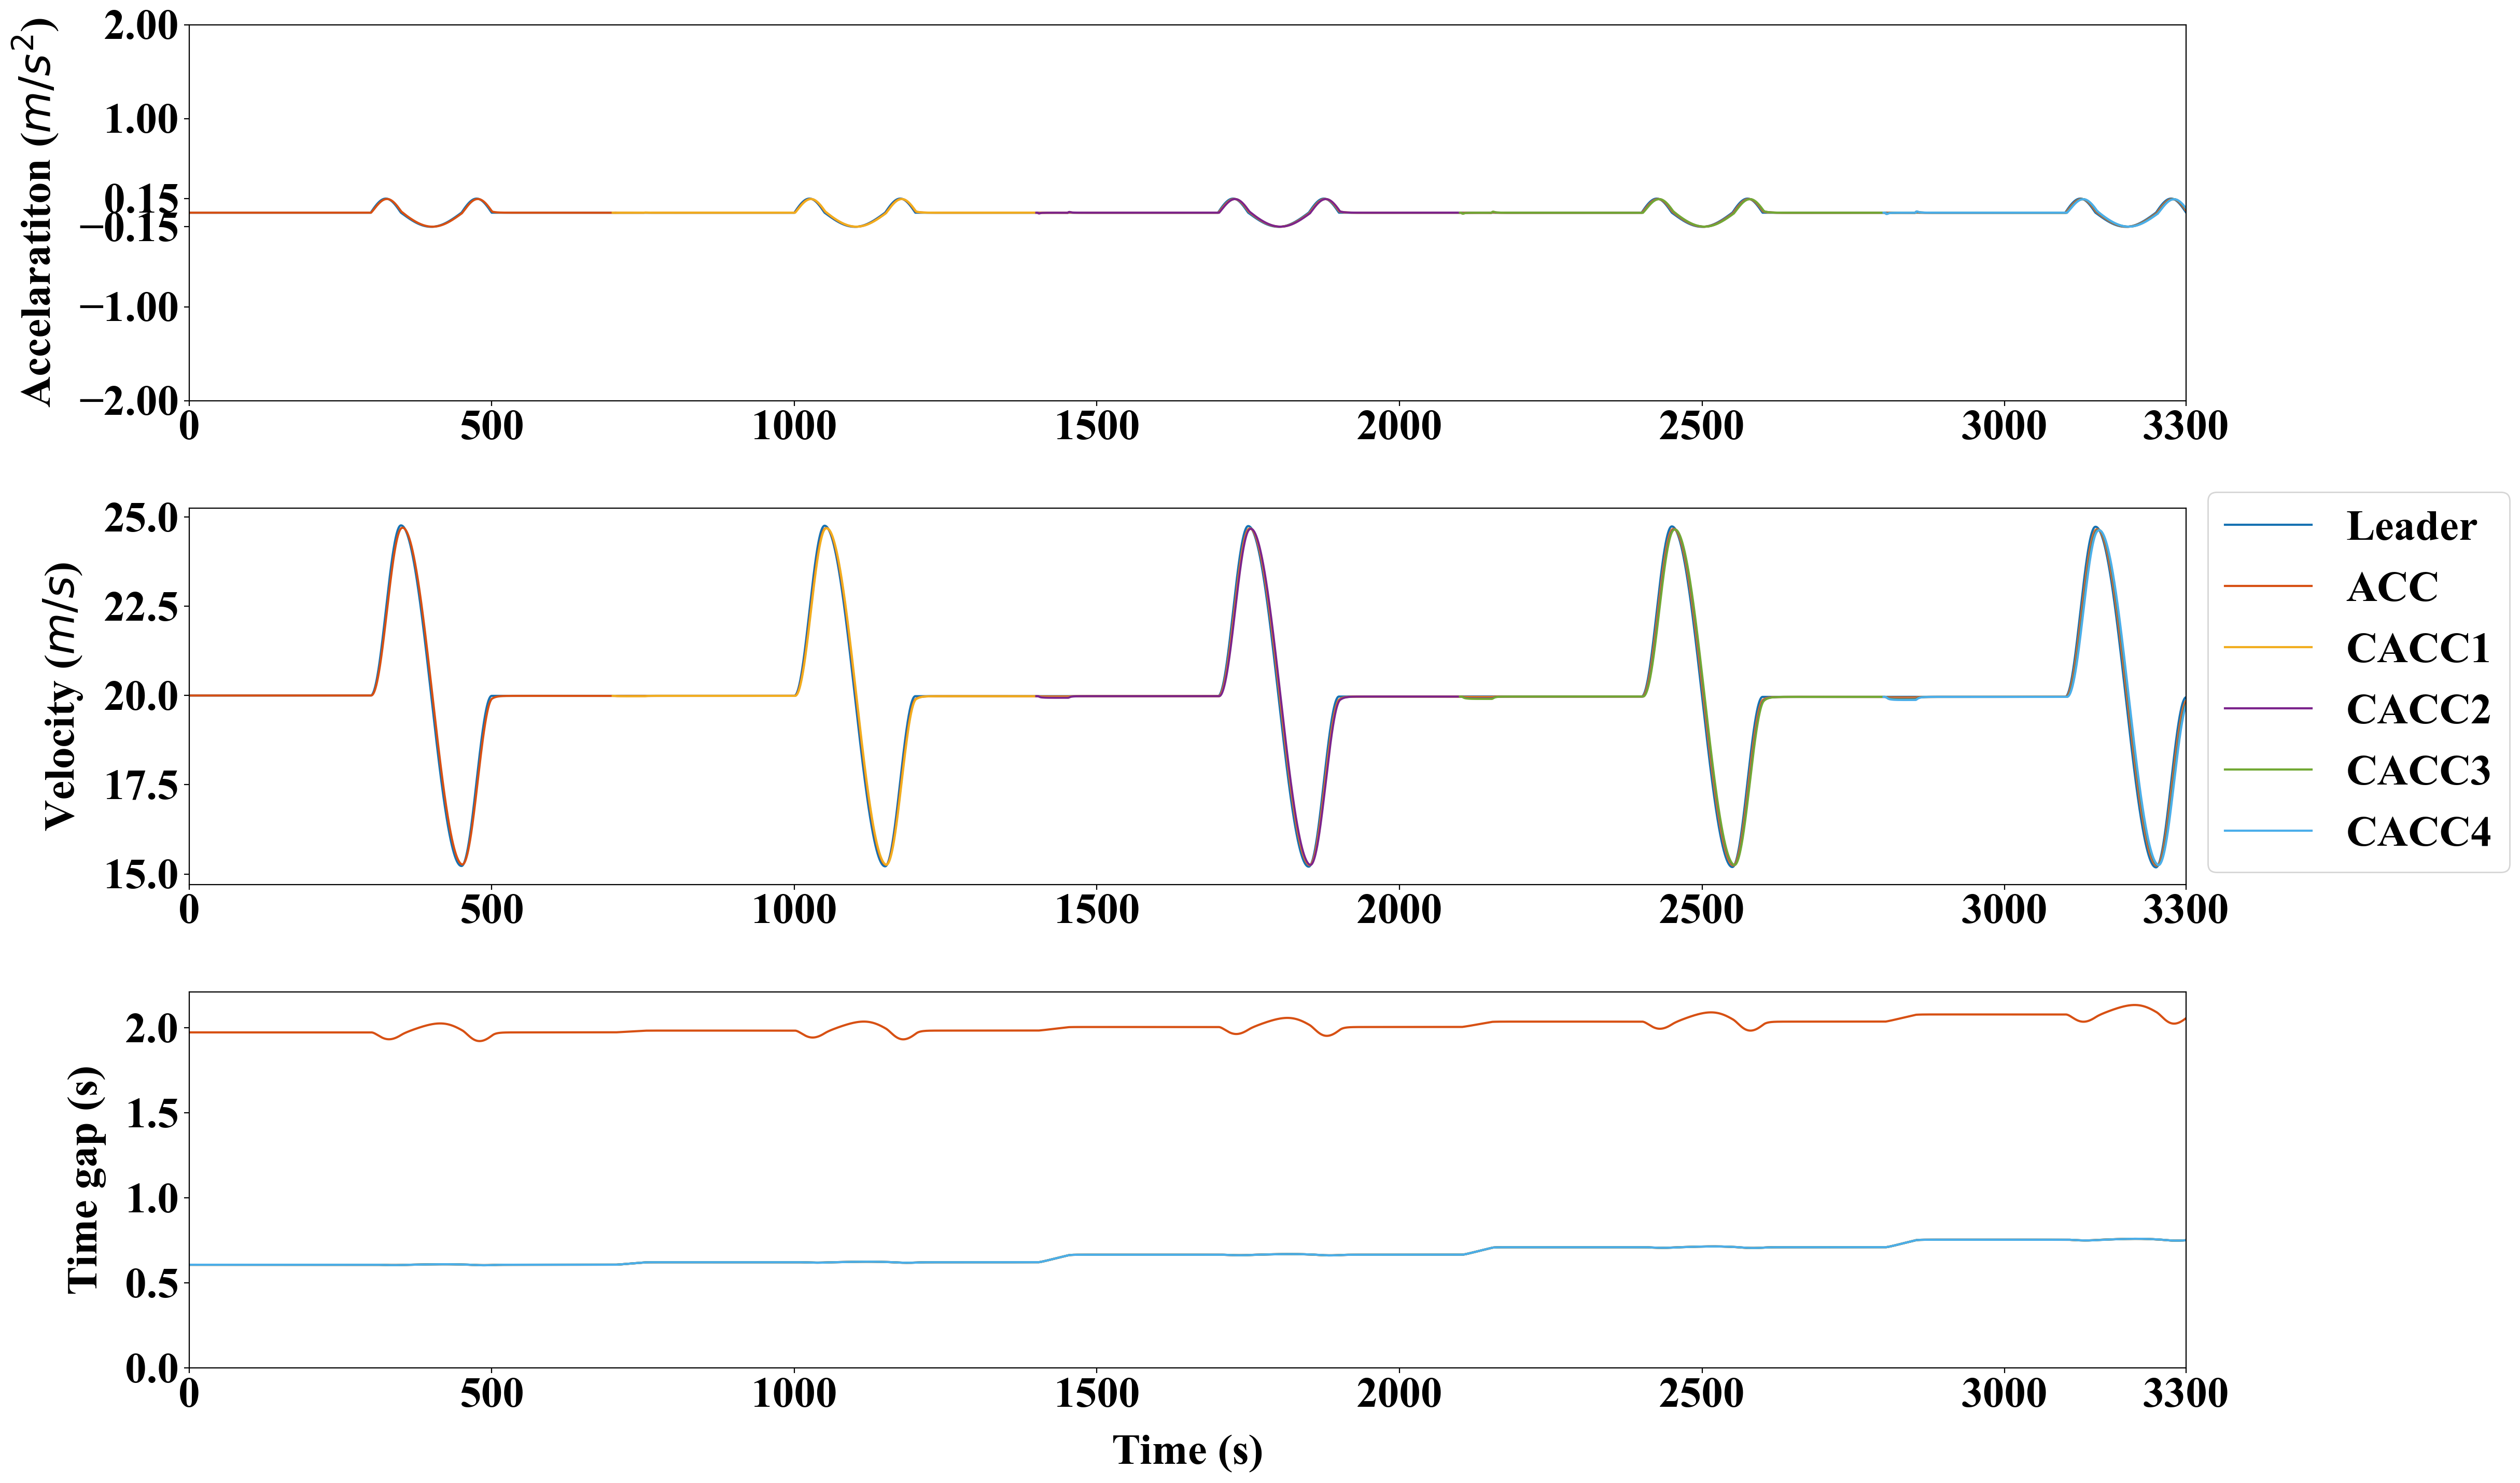
\includegraphics[width=14cm]{figs/extendfig1.png}
% 	\caption{Simulation results of experiment three: CACPC with YK parameterization under the platoon splitting case.}
% 	\label{extend1}
% \end{figure}

% \begin{figure}
% 	\centering
% 		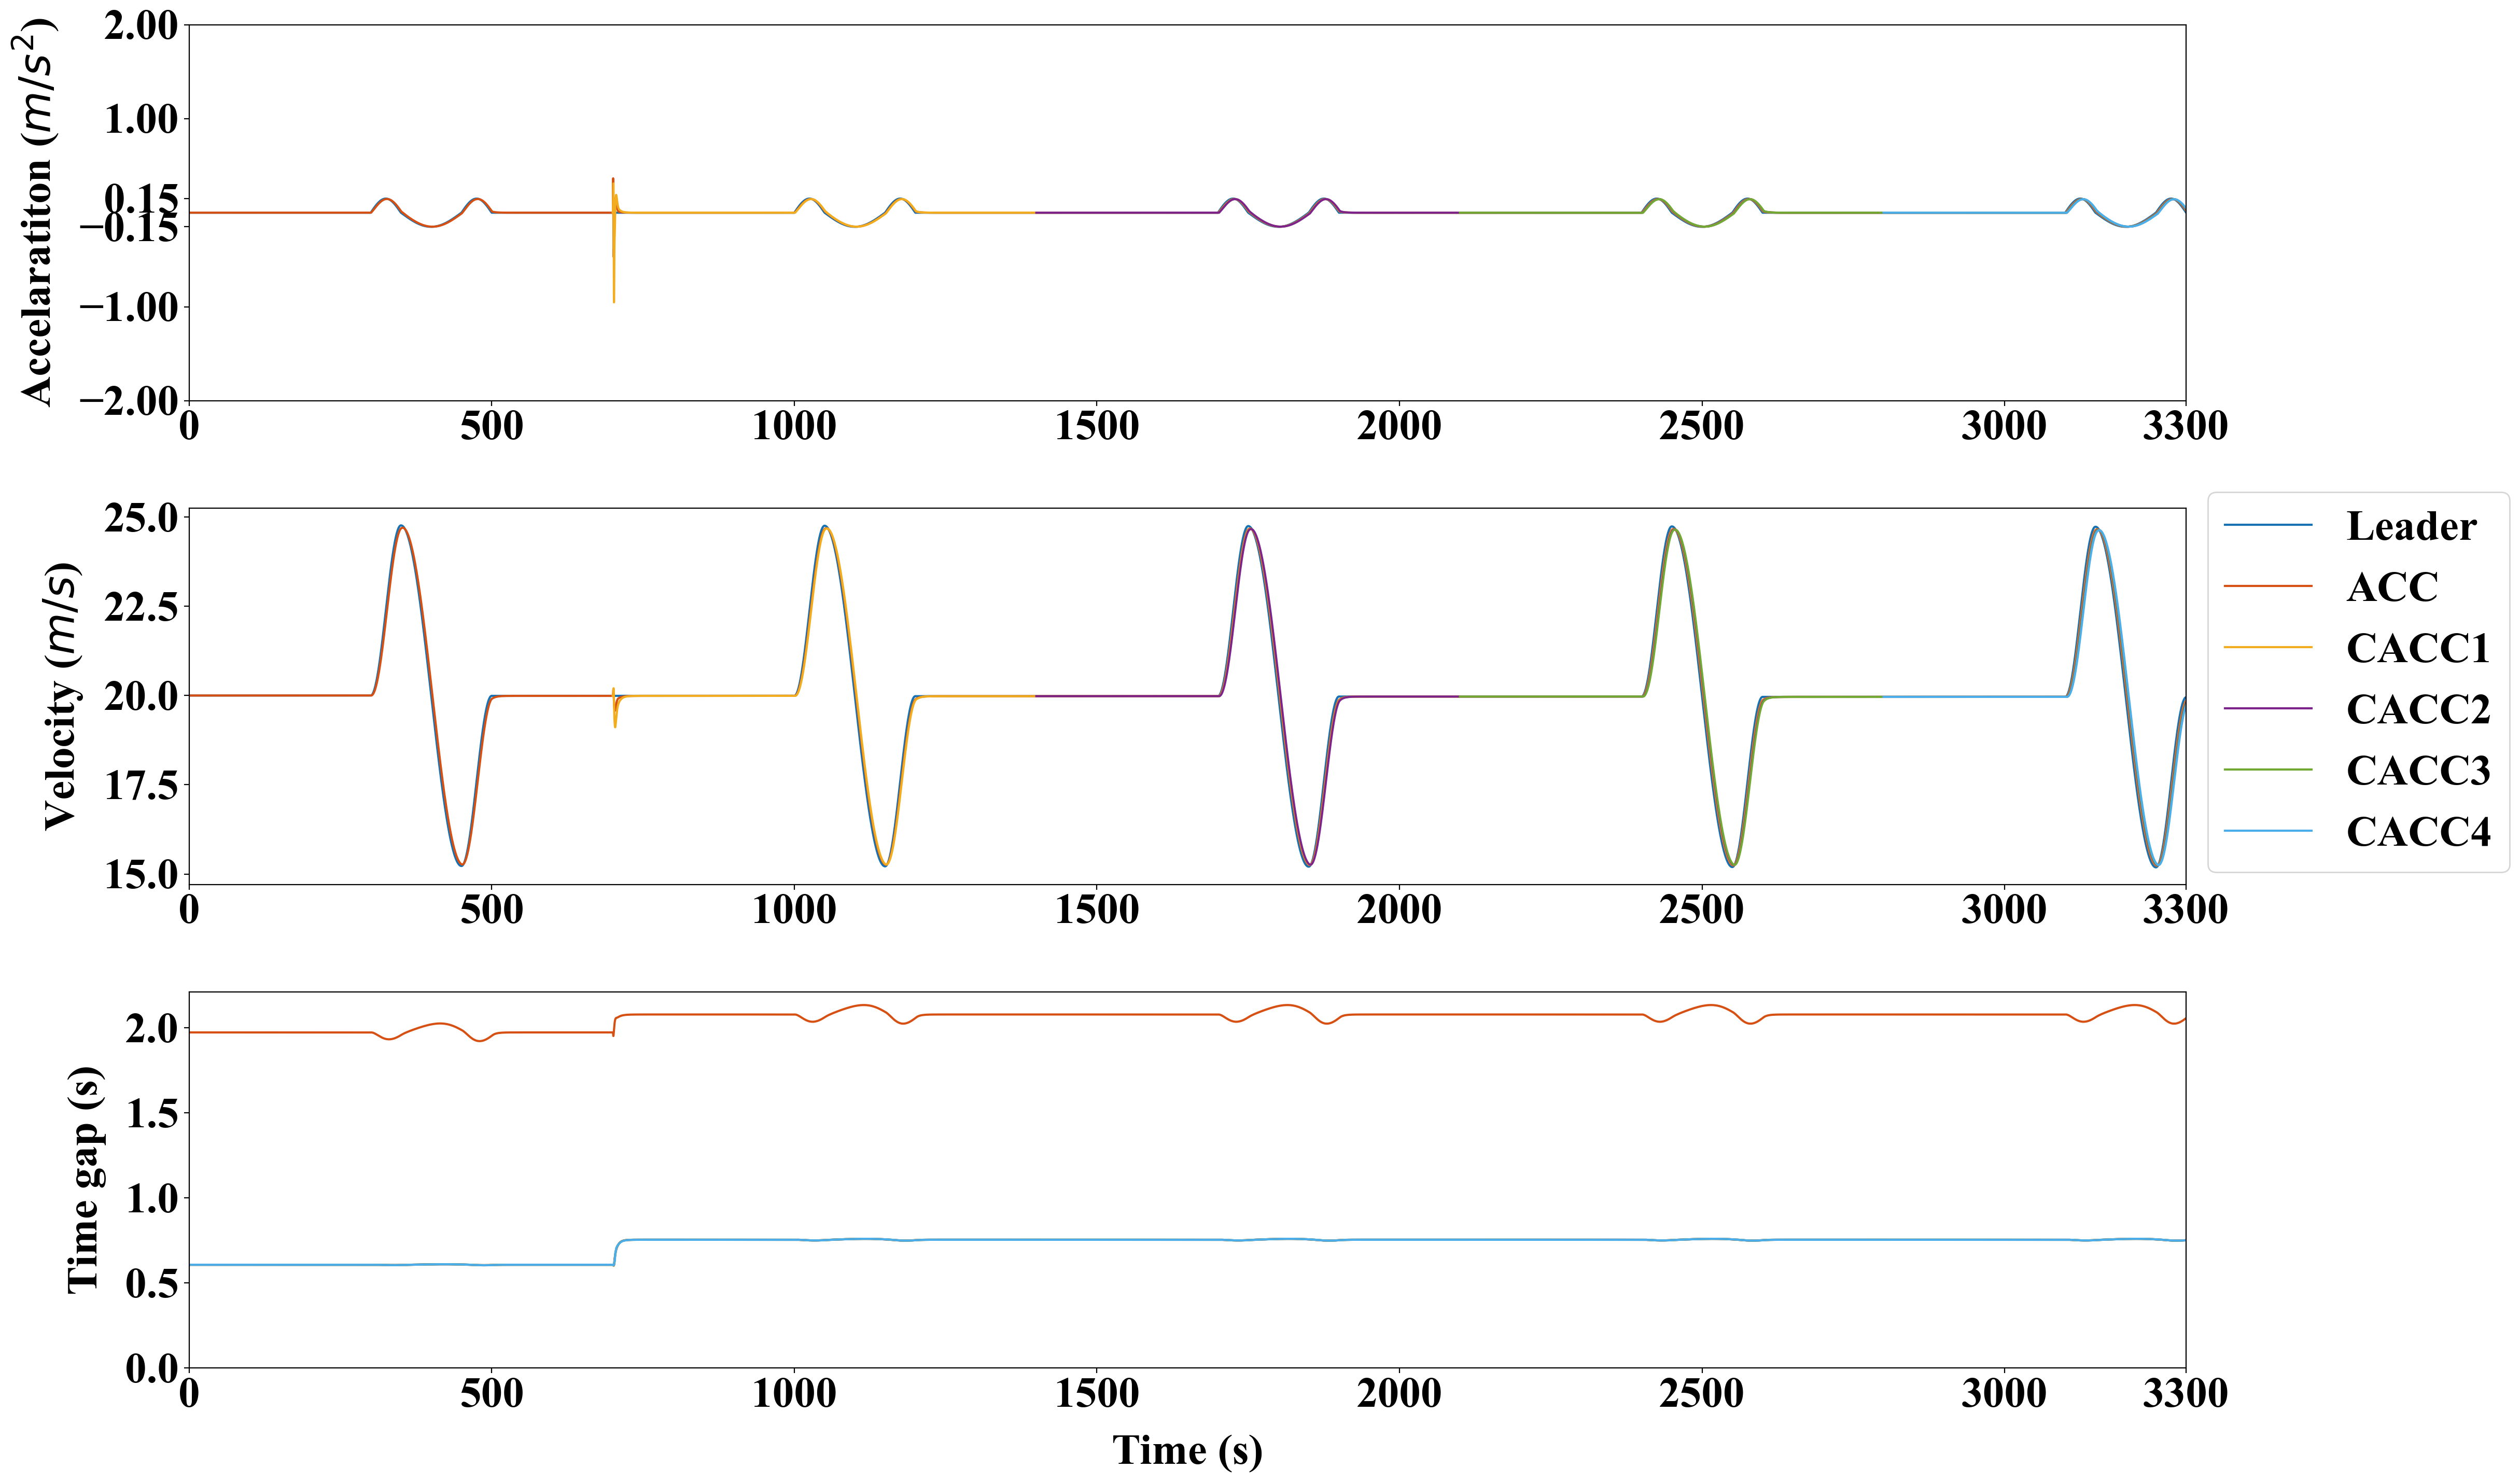
\includegraphics[width=14cm]{figs/extendfig2.png}
% 	\caption{Simulation results of experiment four: CACPC without YK parameterization under the platoon splitting case.}
% 	\label{extend2}
% \end{figure}

% \begin{figure}
% 	\centering
% 		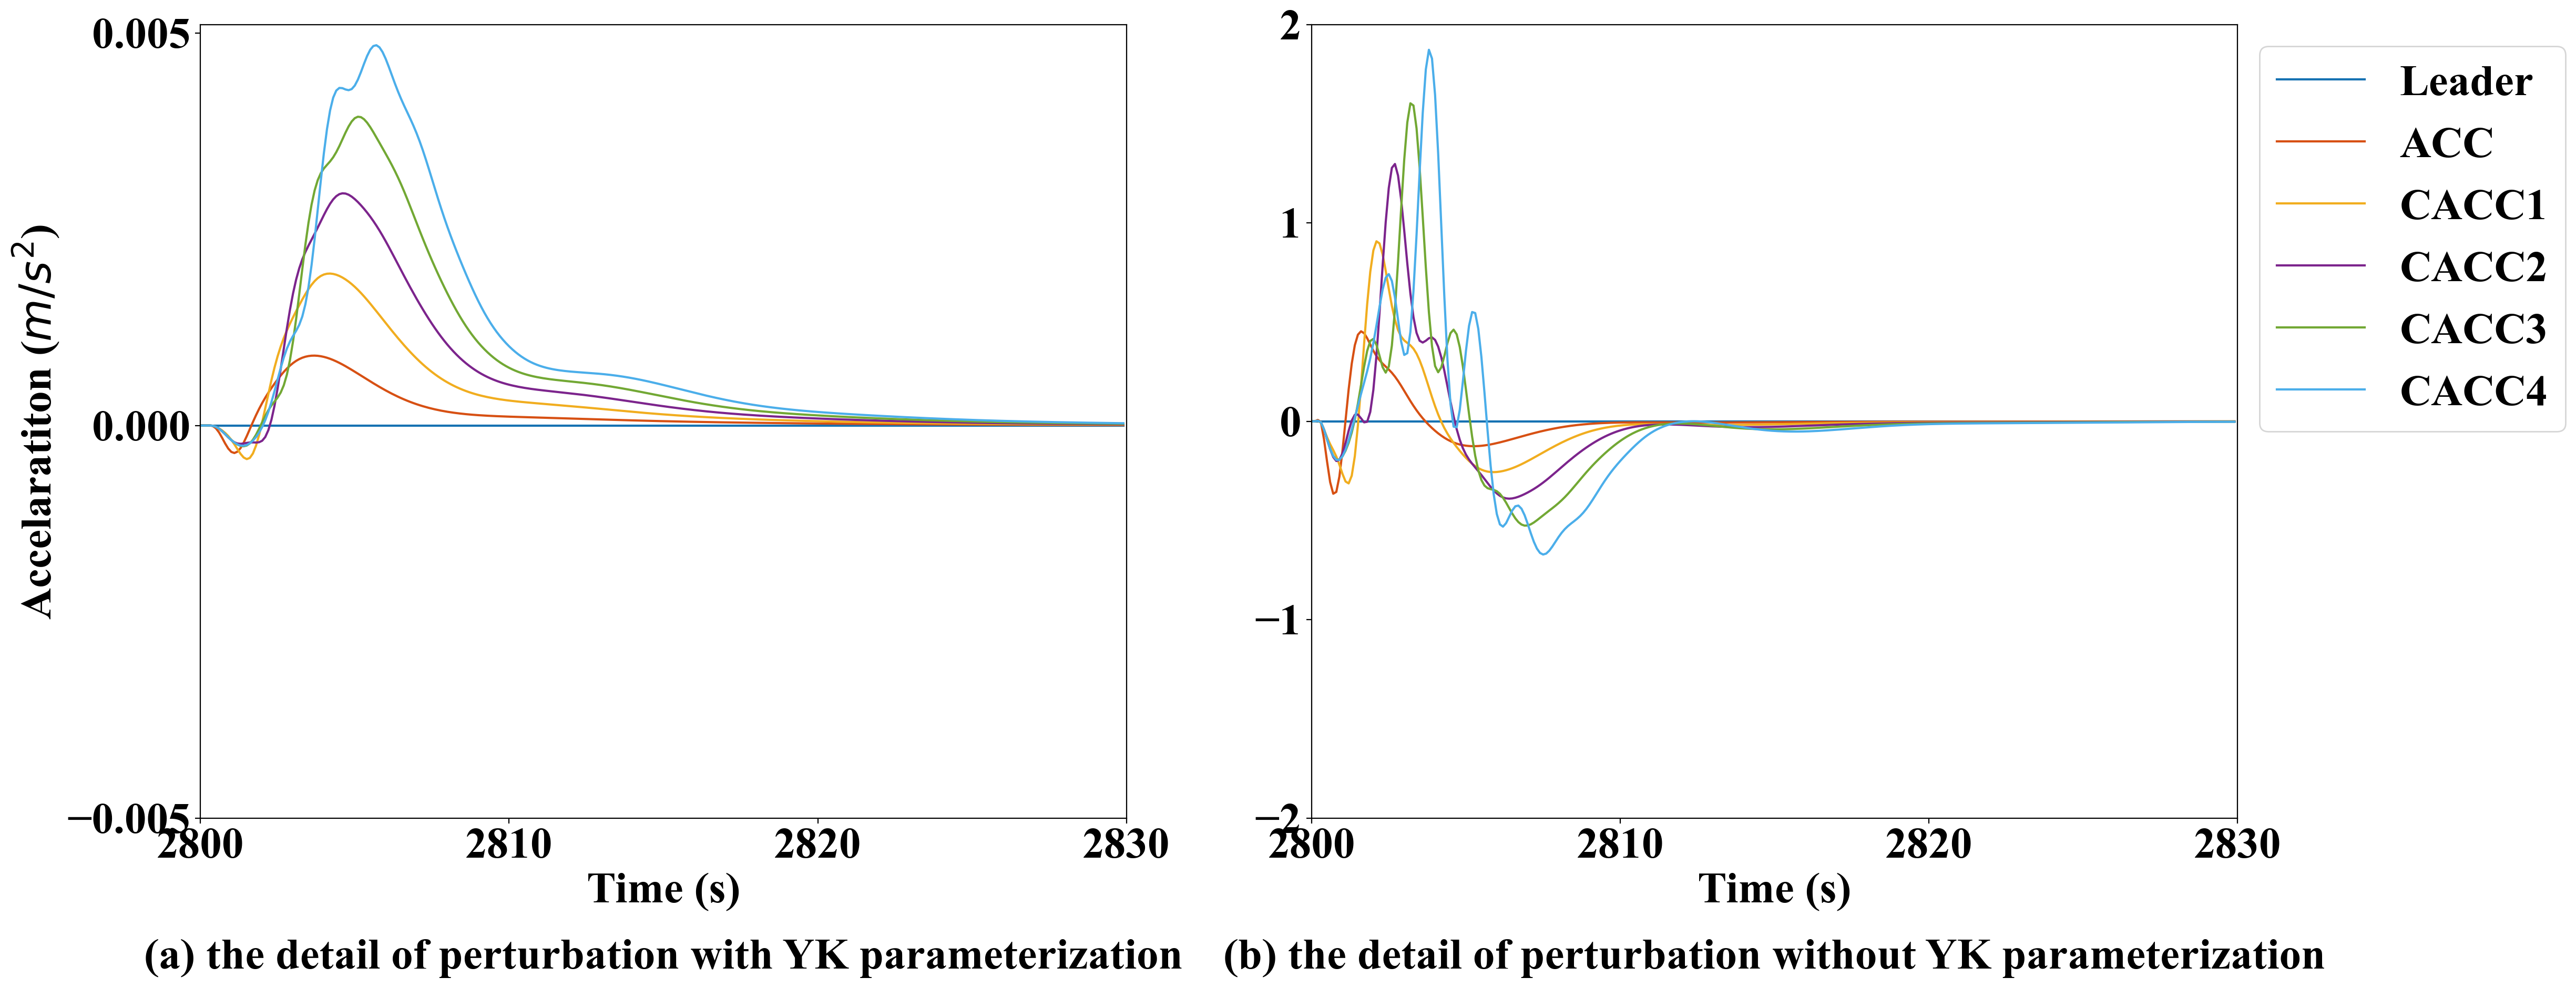
\includegraphics[width=14cm]{figs/extendfig5.png}
% 	\caption{Detailed perturbation simulation results of experiments one and two: CACPC with or without YK parameterization.}
% 	\label{extend5}
% \end{figure}


\textit{Simulation results}. Fig.~\ref{new1} and \ref{new3} show the results of experiments \uppercase\expandafter{\romannumeral1}, \uppercase\expandafter{\romannumeral2}, \uppercase\expandafter{\romannumeral3} and \uppercase\expandafter{\romannumeral4}, respectively. Moreover, Fig.~\ref{new2} and \ref{new4} show the detailed perturbation simulation results of experiments \uppercase\expandafter{\romannumeral1}, \uppercase\expandafter{\romannumeral2}, \uppercase\expandafter{\romannumeral3} and \uppercase\expandafter{\romannumeral4}. In Fig.~\ref{new1} and \ref{new3}, (a)-(c) show the simulation results of the case with YK parameterization and (d)-(f) show the simulation results of the case without YK parameterization where (a),(d) Acceleration of simulation results; (b),(e) Velocity of simulation results; (c),(f) Time gap of simulation results. As for Fig.~\ref{new2} and \ref{new4}, (a)-(e) show the propagating processes of five applied perturbations and (f)-(i) show the four switching processes of the case with YK parameterization. Furthermore, for the case without YK parameterization, (j)-(n) show the propagating processes of five applied perturbations, and (o)-(r) show the four switching processes.

In Fig.~\ref{new1} and \ref{new2}, the process of the gradual formation of the CACC platoon with and without YK parameterization is clearly shown, while the process of the gradual splitting is shown in Fig.~\ref{new3} and \ref{new4}. The first attention is spontaneous perturbations during controller switching. From the comparison of Fig.~\ref{new2} and \ref{new4}, we can find that the controller switching causes spontaneous perturbations in the process of platoon formation, which is caused by the changing of the equivalent desired time gap. These spontaneous perturbations can be suppressed by applying the tuning function $\gamma$ to achieve smooth switching. Specifically, the maximum magnitude of the perturbation is reduced from $2 m/s^{2}$ to $0.011 m/s^{2}$ by YK parameterization. However, in the case without YK parameterization, due to the direct switching when the platoon size reaches or leaves the trigger size, the spontaneous perturbation is significant, which seriously impacts the stability and safety of the traffic flow. The second attention is string stability. All CACPCs applied under different CACC platoon sizes can maintain string stability through YK parameterization which are shown in Fig.~\ref{new2} and \ref{new4}. Furthermore, the subplots of the time gap in Fig.~\ref{new1} and \ref{new3} illustrate that with YK parameterization, the time gap decreases as the platoon size increases. However, without YK parameterization, the time gap does not change significantly with the change in platoon size unless the specified platoon size is reached. Therefore, it can be concluded that with YK parameterization, the platoon control mode can be effective regardless of the platoon size so that it does not limit the gain of CACCs for traffic flow.


Moreover, YK parameterization can work under any CACC MPR since it can be applied even in a typical scenario where the CACC MPR is low and the platoon size is small. Nevertheless, for the case without YK parameterization, the CACPCs do not function sufficiently until the set trigger platoon size is reached, which means it is hard to function for a long period because there will be a long time until the CACC MPR gets high. In addition, because the splitting and forming processes are similar, the following simulation experiments are only conducted in the forming process. Notice that from the difference in the acceleration between subplot (a) and (b) in Fig.~\ref{new1} and \ref{new3}, which is detailed shown in subplot (k)-(r) in Fig.~\ref{new2} and \ref{new4}, a misunderstood conclusion can be drawn because the perturbation is amplified with or without YK parameterization. However, the perturbation is caused by the equivalent desired time gap increase during the controller switching. In the case with YK parameterization, the perturbation only rises once and then back to the equivalent state. On the contrary, for the case without YK parameterization, the perturbation fluctuates during the propagating process, which means the switching progress is not smooth enough to suppress the perturbation.

\subsubsection{Simulation experiments maintain a fluctuating speed during the forming process}
\label{Section 5.2.2}
~\\

\textit{Simulation scenario:} The simulation scenario is similar to experiment \uppercase\expandafter{\romannumeral1} in Section.~\ref{Section 5.2.1}, but different in the given speed and acceleration configuration of the leader vehicle. In this simulation experiment, the speed of the leader vehicle fluctuates all the time to simulate the traffic oscillation scenario. There are two experiments conducted:
\begin{enumerate}
  \item \textit{Experiment \uppercase\expandafter{\romannumeral5}:} The forming process of the CACC platoon with YK parameterization under the fluctuating velocity case where an ACC (which is a CACC but degraded to an ACC functionally) follows the leader at the beginning, and more CACCs join the CACC platoon one by one at the simulation time of 700s, 1400s, 2100s, and 2800s.
  \item \textit{Experiment \uppercase\expandafter{\romannumeral6}:} The forming process of the CACC platoon without YK parameterization under the fluctuating velocity case where an ACC (which is a CACC but degraded to an ACC functionally) follows the leader at the beginning, and more CACCs join the CACC platoon one by one at the simulation time of 700s, 1400s, 2100s, and 2800s. Note that since the fixed platoon control only functions when the platoon size reaches 5, the platoon control without YK parameterization is enabled after 2800s.
\end{enumerate}

\begin{figure}
  \centering
  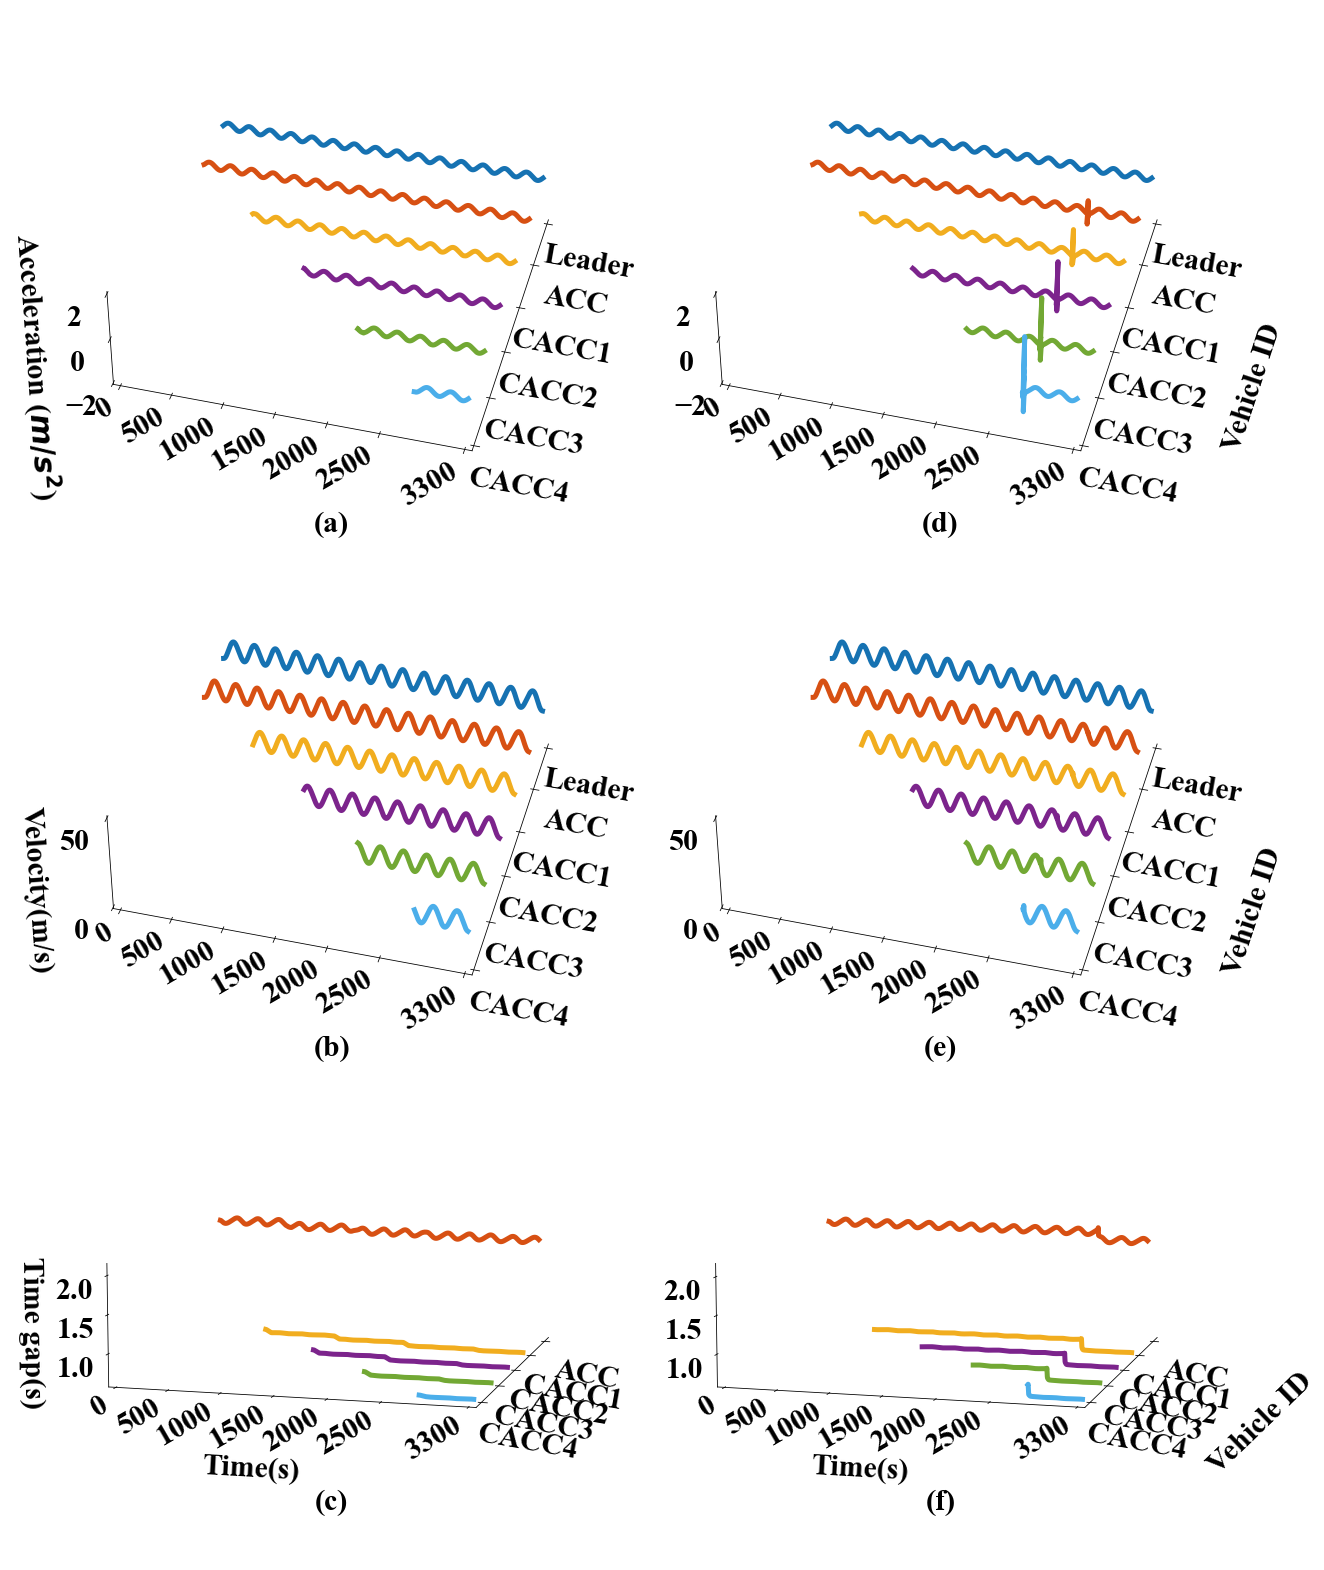
\includegraphics[width=8.5cm]{figs/f_YK_form.png}
  \caption{~Simulation results of experiments \uppercase\expandafter{\romannumeral5} and \uppercase\expandafter{\romannumeral6}: CACPC with or without YK parameterization under the fluctuating velocity case. (a)-(c) show the simulation results of experiment \uppercase\expandafter{\romannumeral5}, and (d)-(f) show the simulation results of experiment \uppercase\expandafter{\romannumeral6}. (a),(d) Acceleration of simulation results; (b),(e) Velocity of simulation results; (c),(f) Time gap of simulation results.}
  \label{new5}
\end{figure}

\begin{figure}
  \centering
  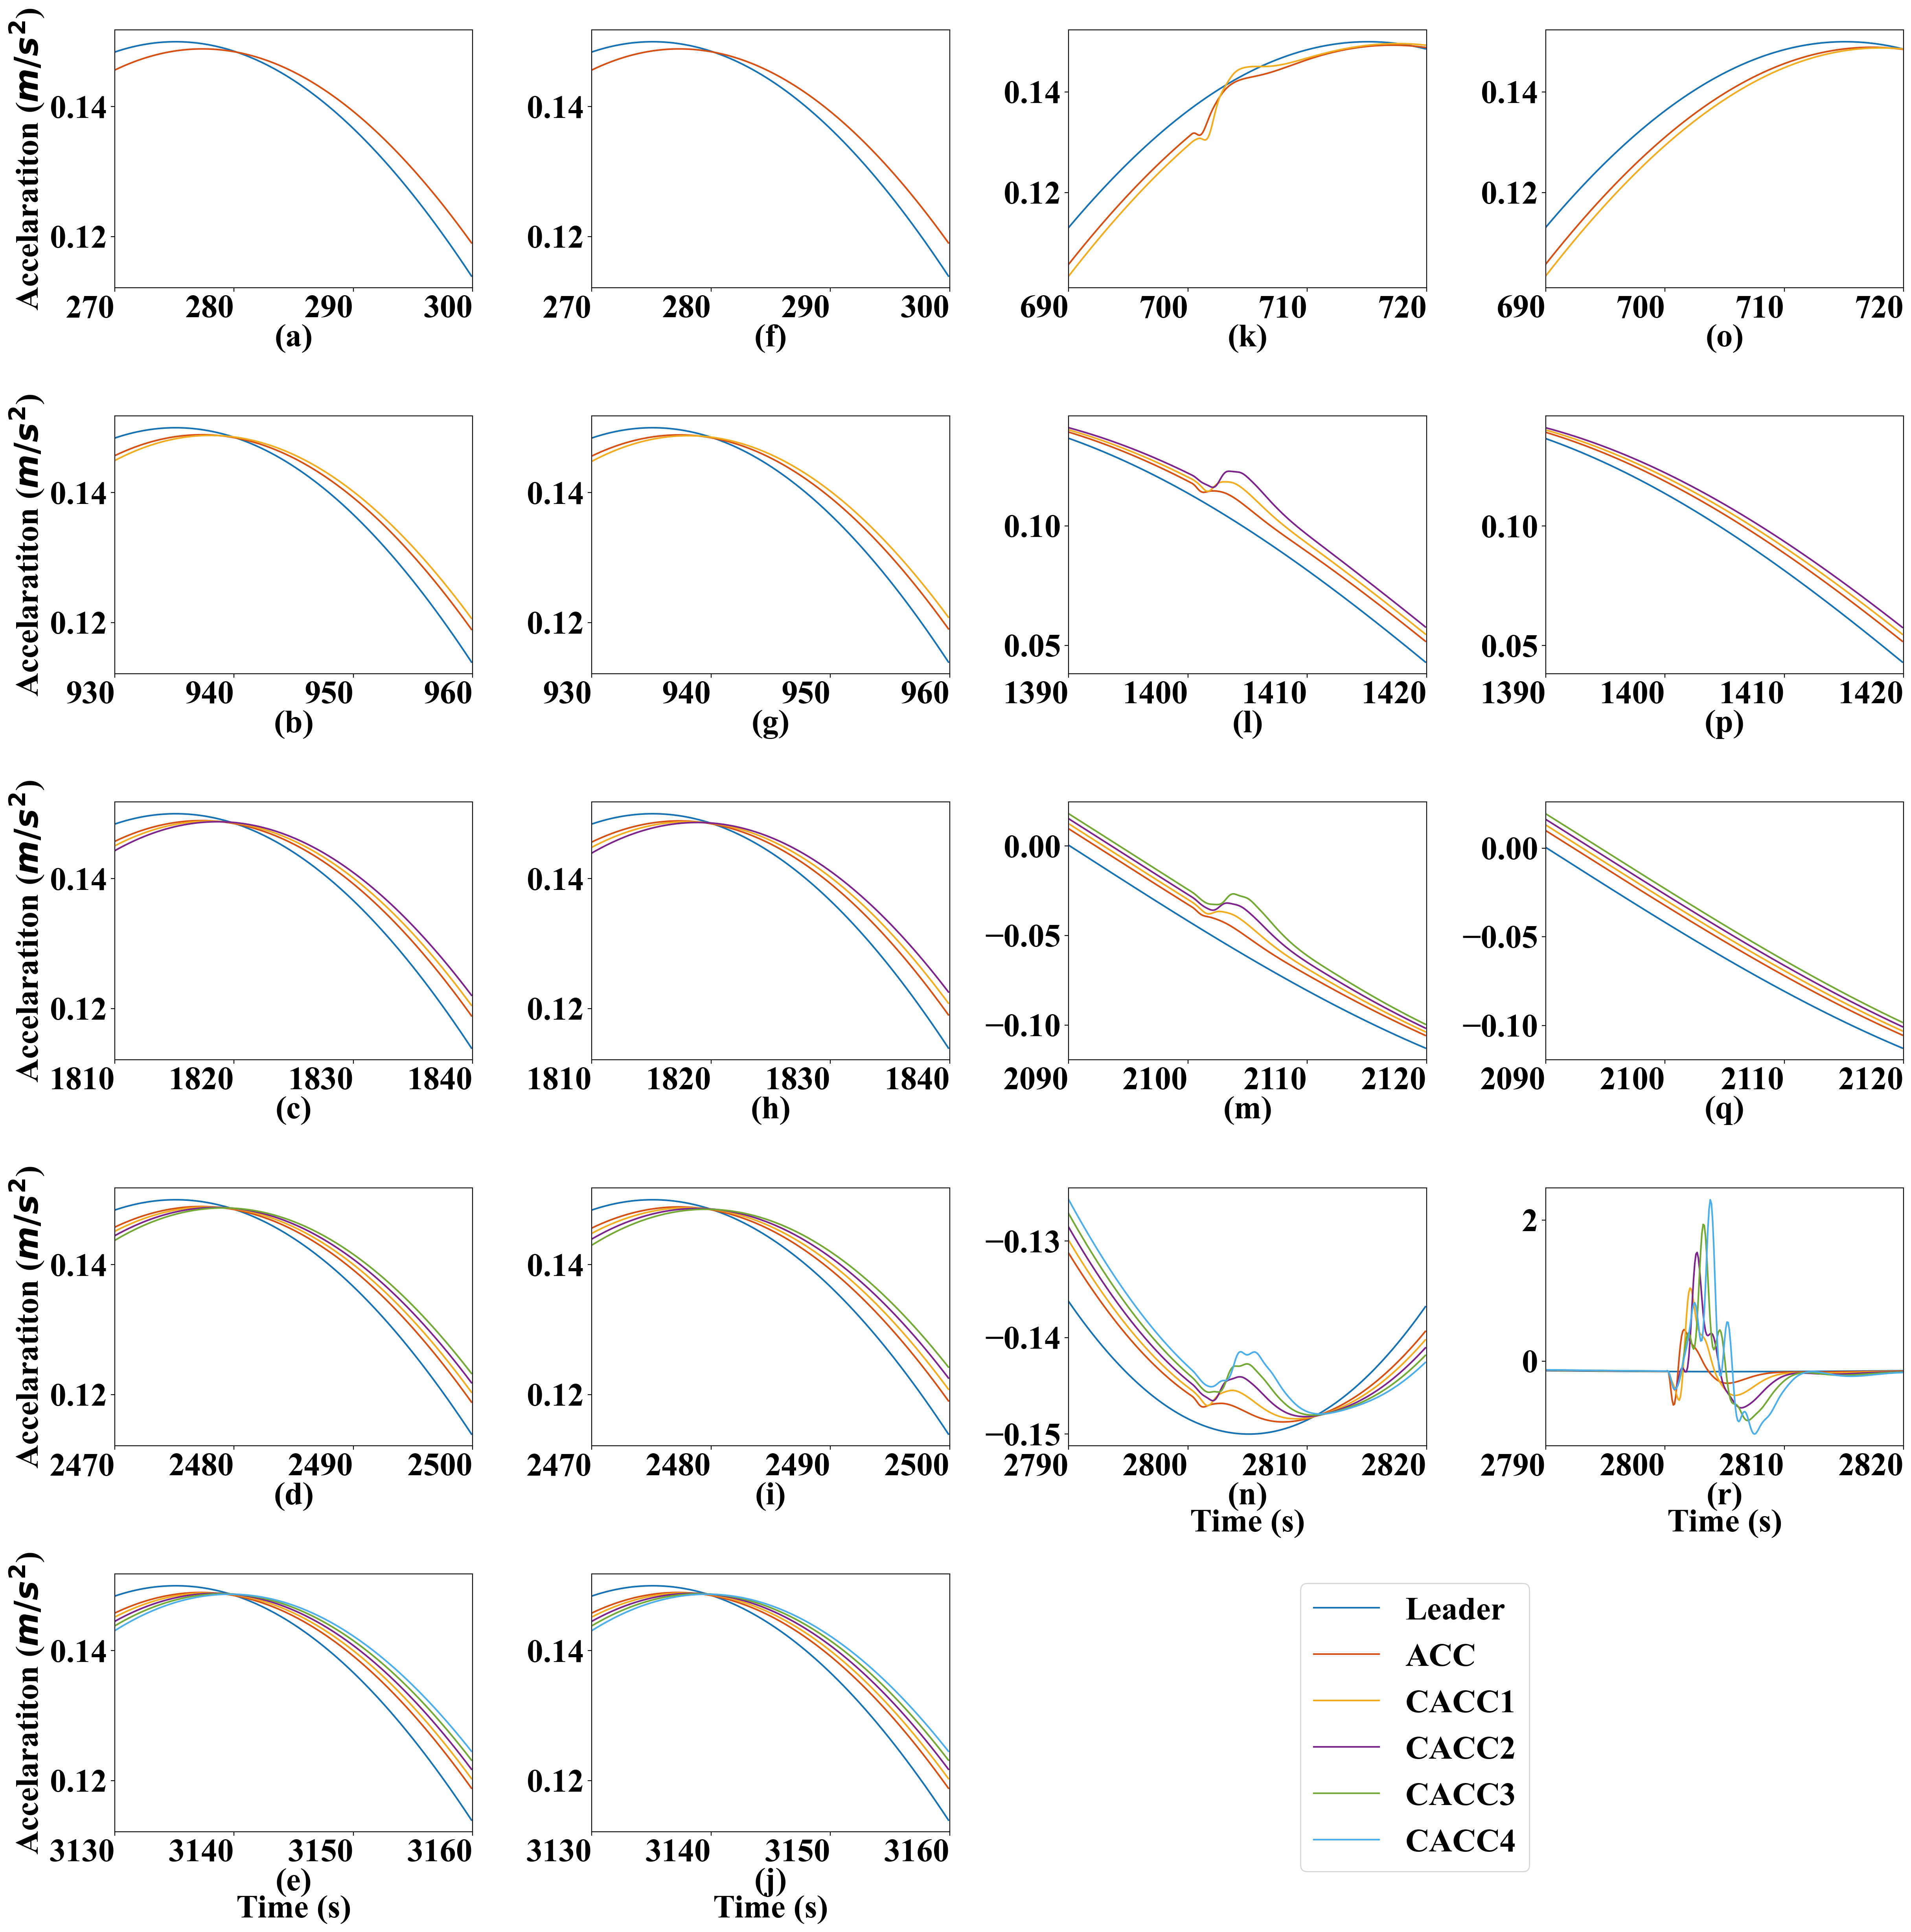
\includegraphics[width=8.5cm]{figs/fluat_detail.png}
  \caption{~Detailed perturbation simulation results of experiments \uppercase\expandafter{\romannumeral5} and \uppercase\expandafter{\romannumeral6}: CACPC with or without YK parameterization under the fluctuating velocity case. For experiment \uppercase\expandafter{\romannumeral5}, (a)-(e) show the propagating processes of five applied perturbations, and (k)-(l) show the four switching processes. For experiment \uppercase\expandafter{\romannumeral6}, (f)-(j) show the propagating processes of five applied perturbations, and (o)-(r) show the four switching processes.}
  \label{new6}
\end{figure}

% \begin{figure}
% 	\centering
% 		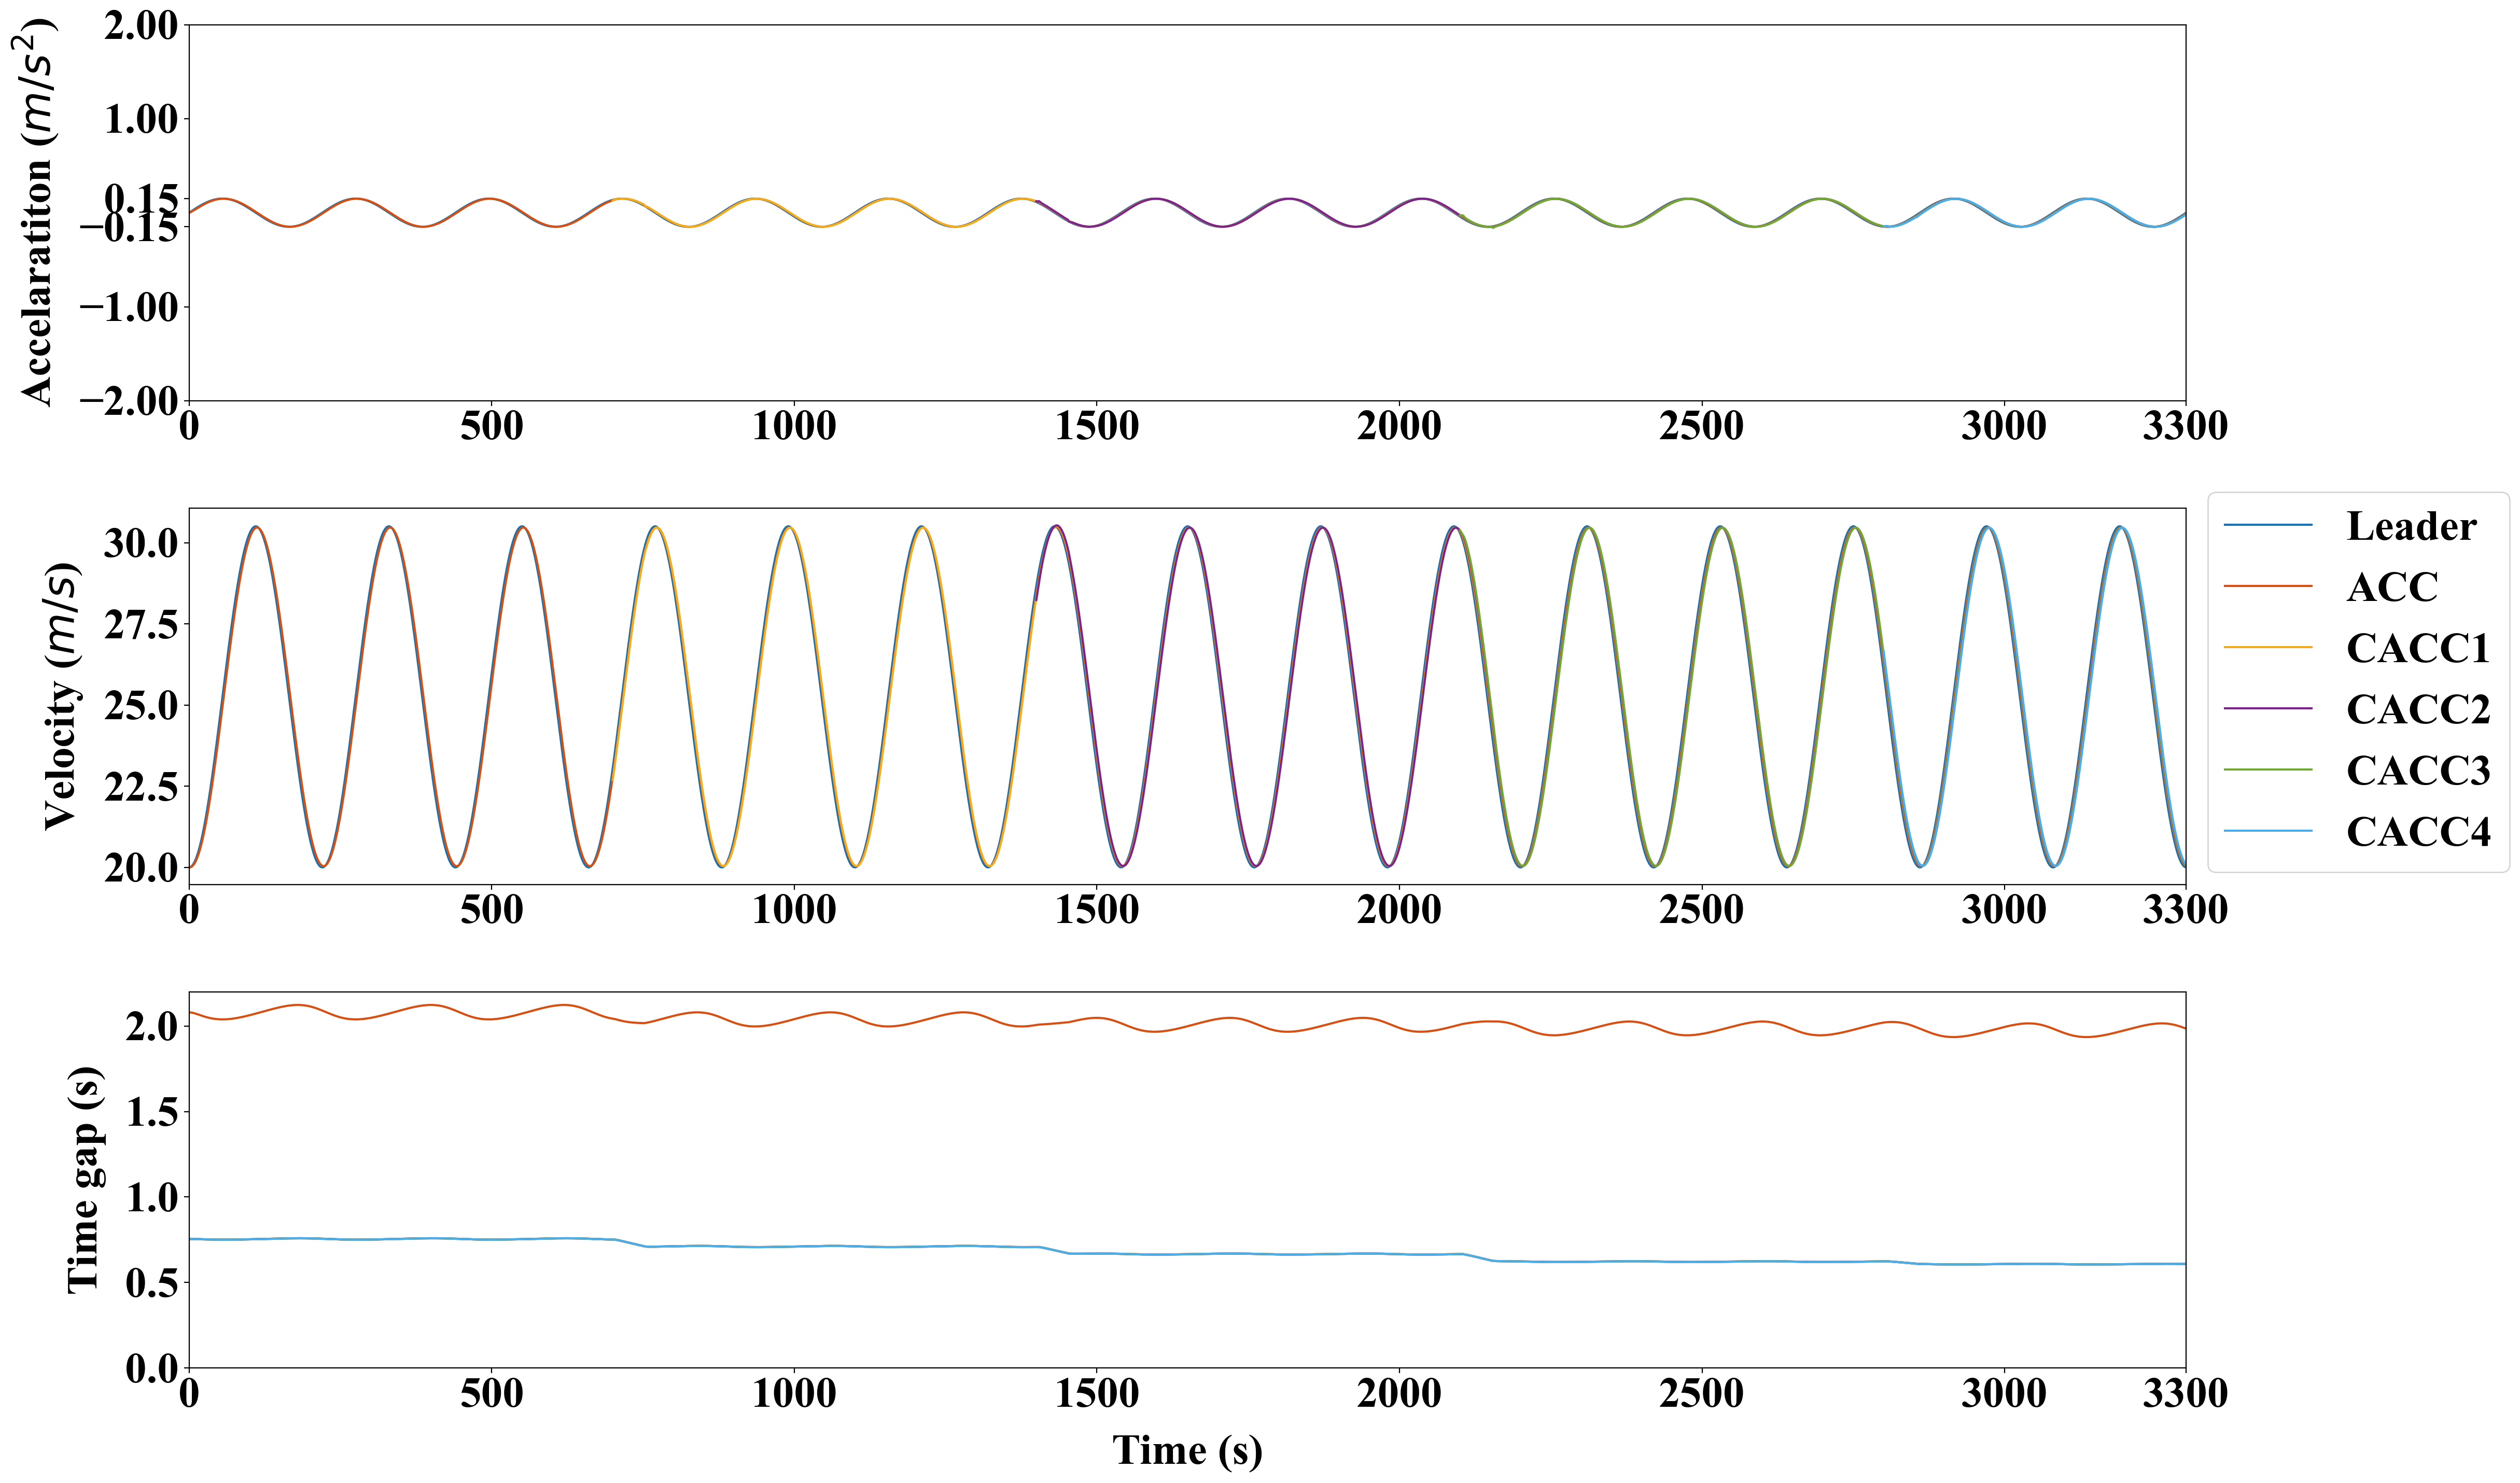
\includegraphics[width=14cm]{figs/extendfig3.png}
% 	\caption{~Simulation results of experiment five: CACPC with YK parameterization under the platoon forming case.}
% 	\label{extend3}
% \end{figure}

% \begin{figure}
% 	\centering
% 		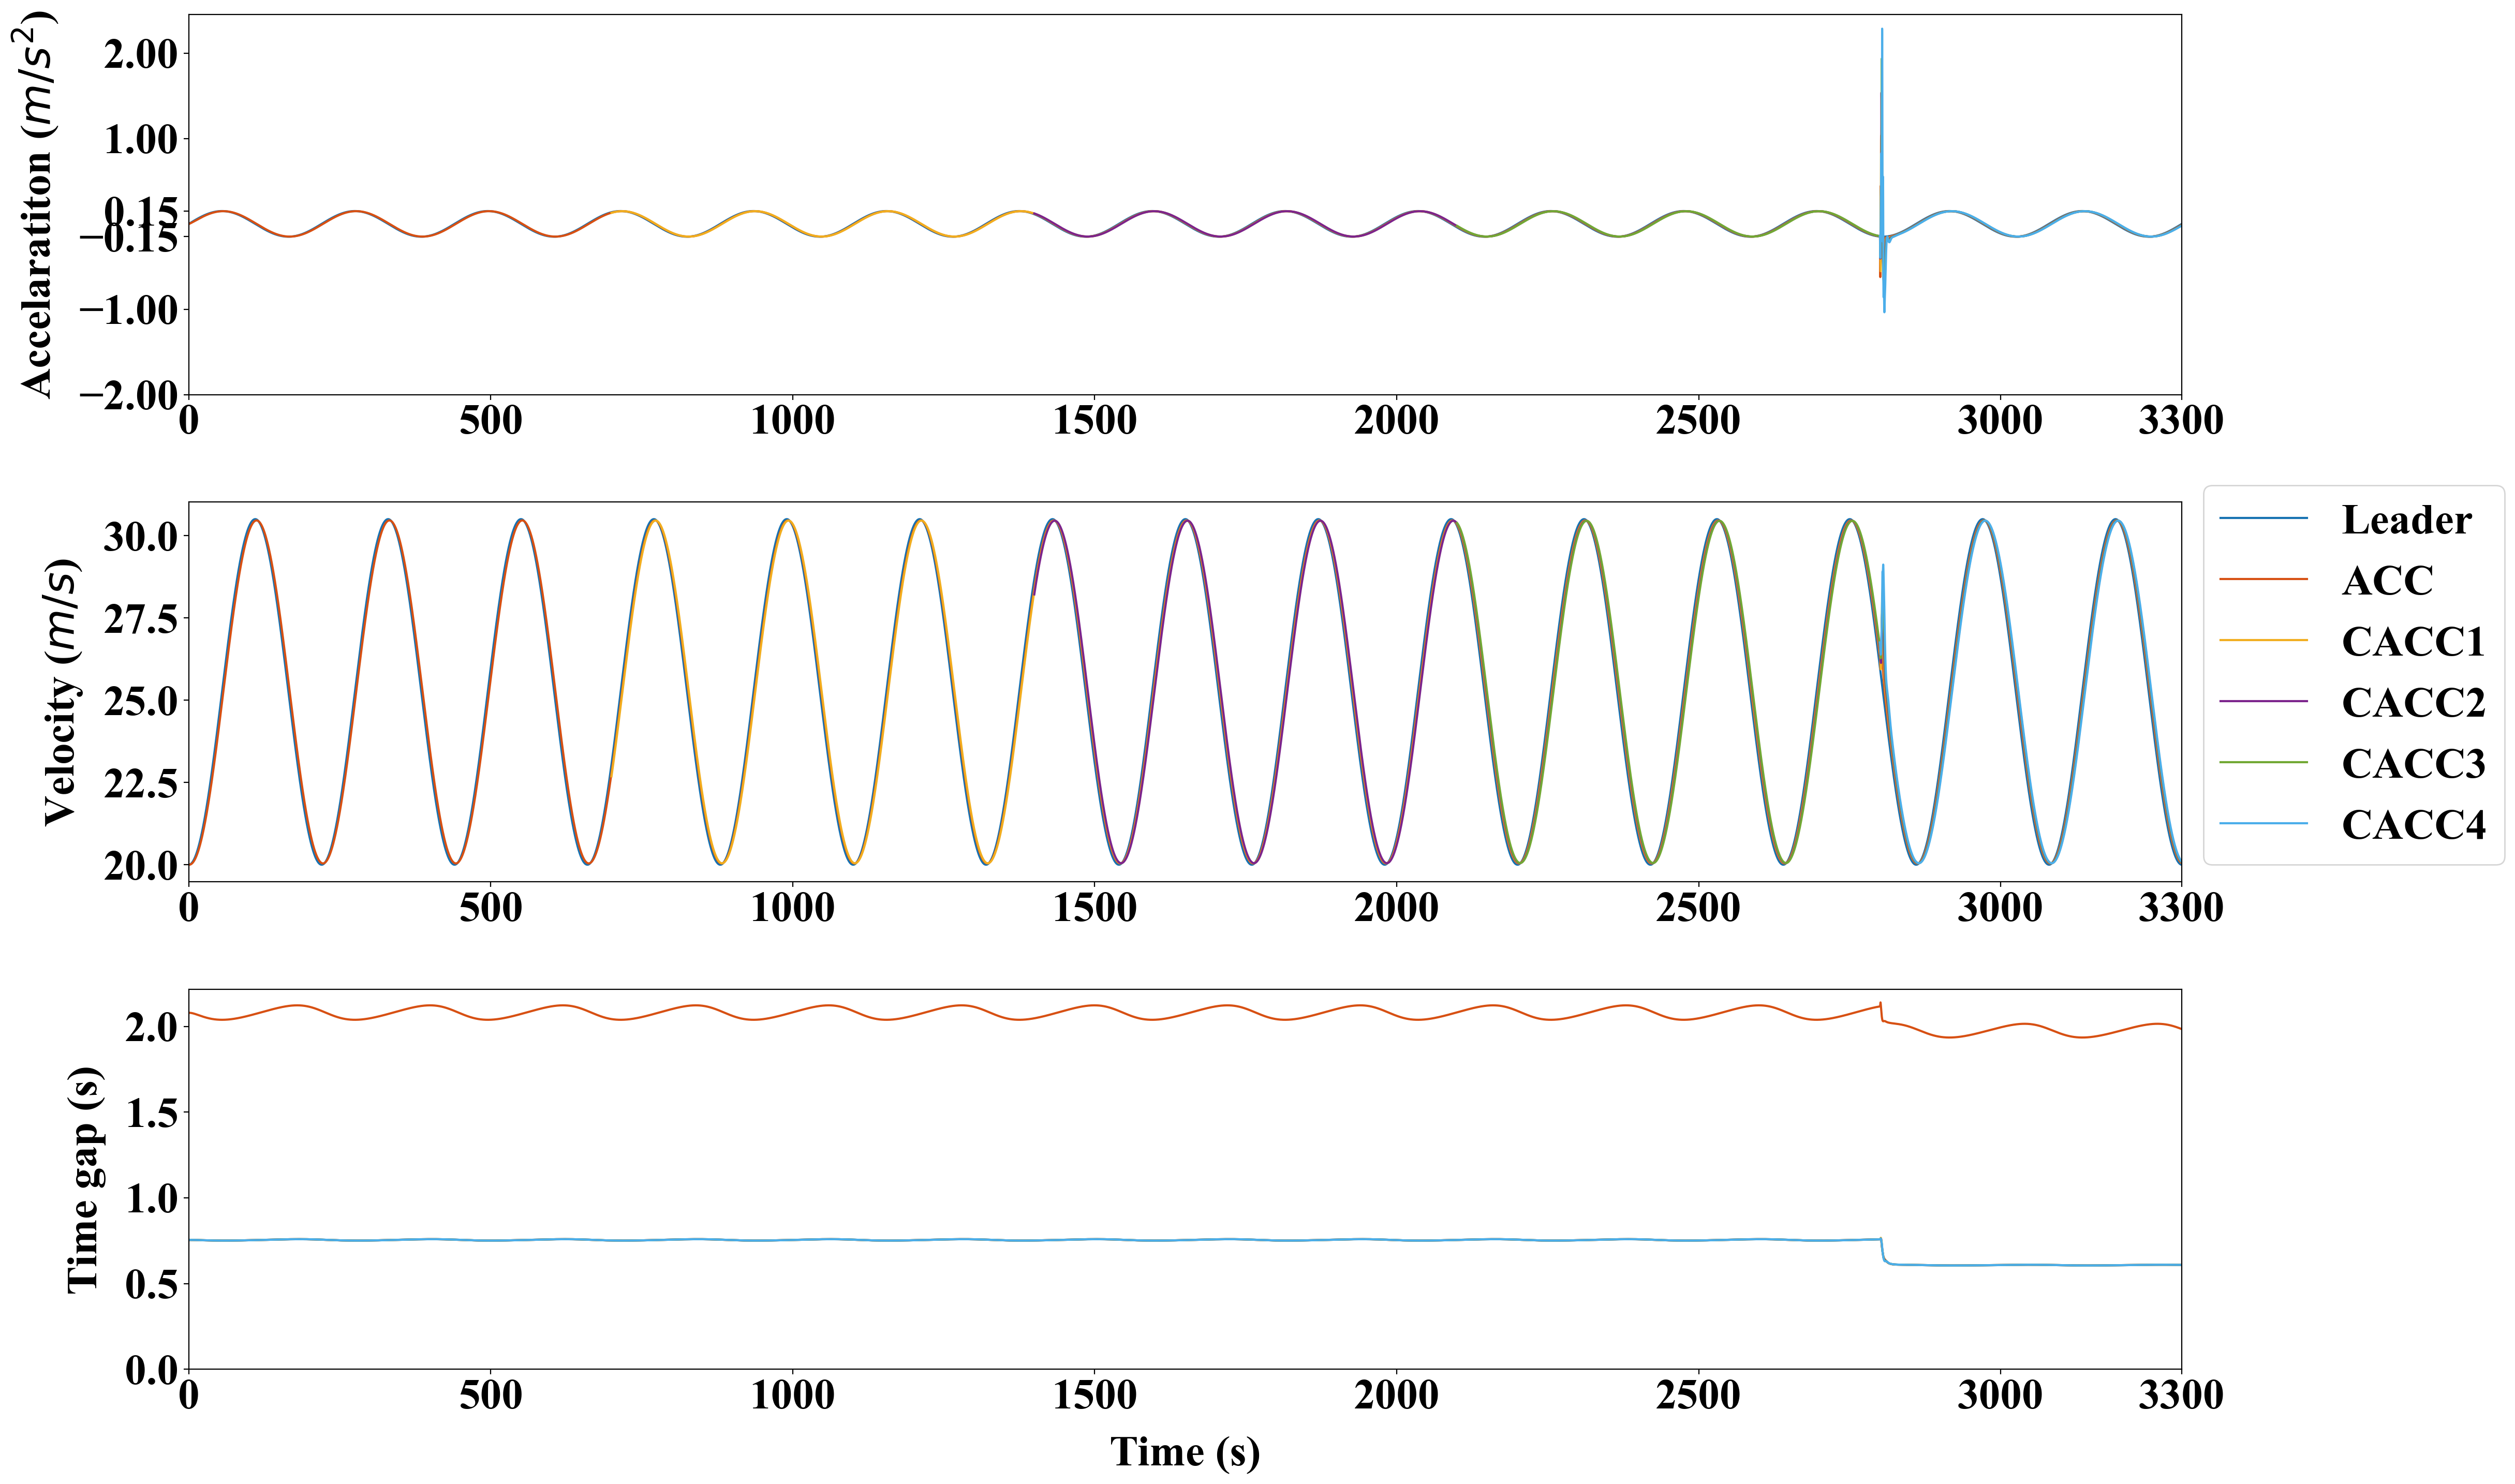
\includegraphics[width=14cm]{figs/extendfig4.png}
% 	\caption{~Simulation results of experiment six: CACPC without YK parameterization under the platoon forming case.}
% 	\label{extend4}
% \end{figure}

% \begin{figure}
% 	\centering
% 		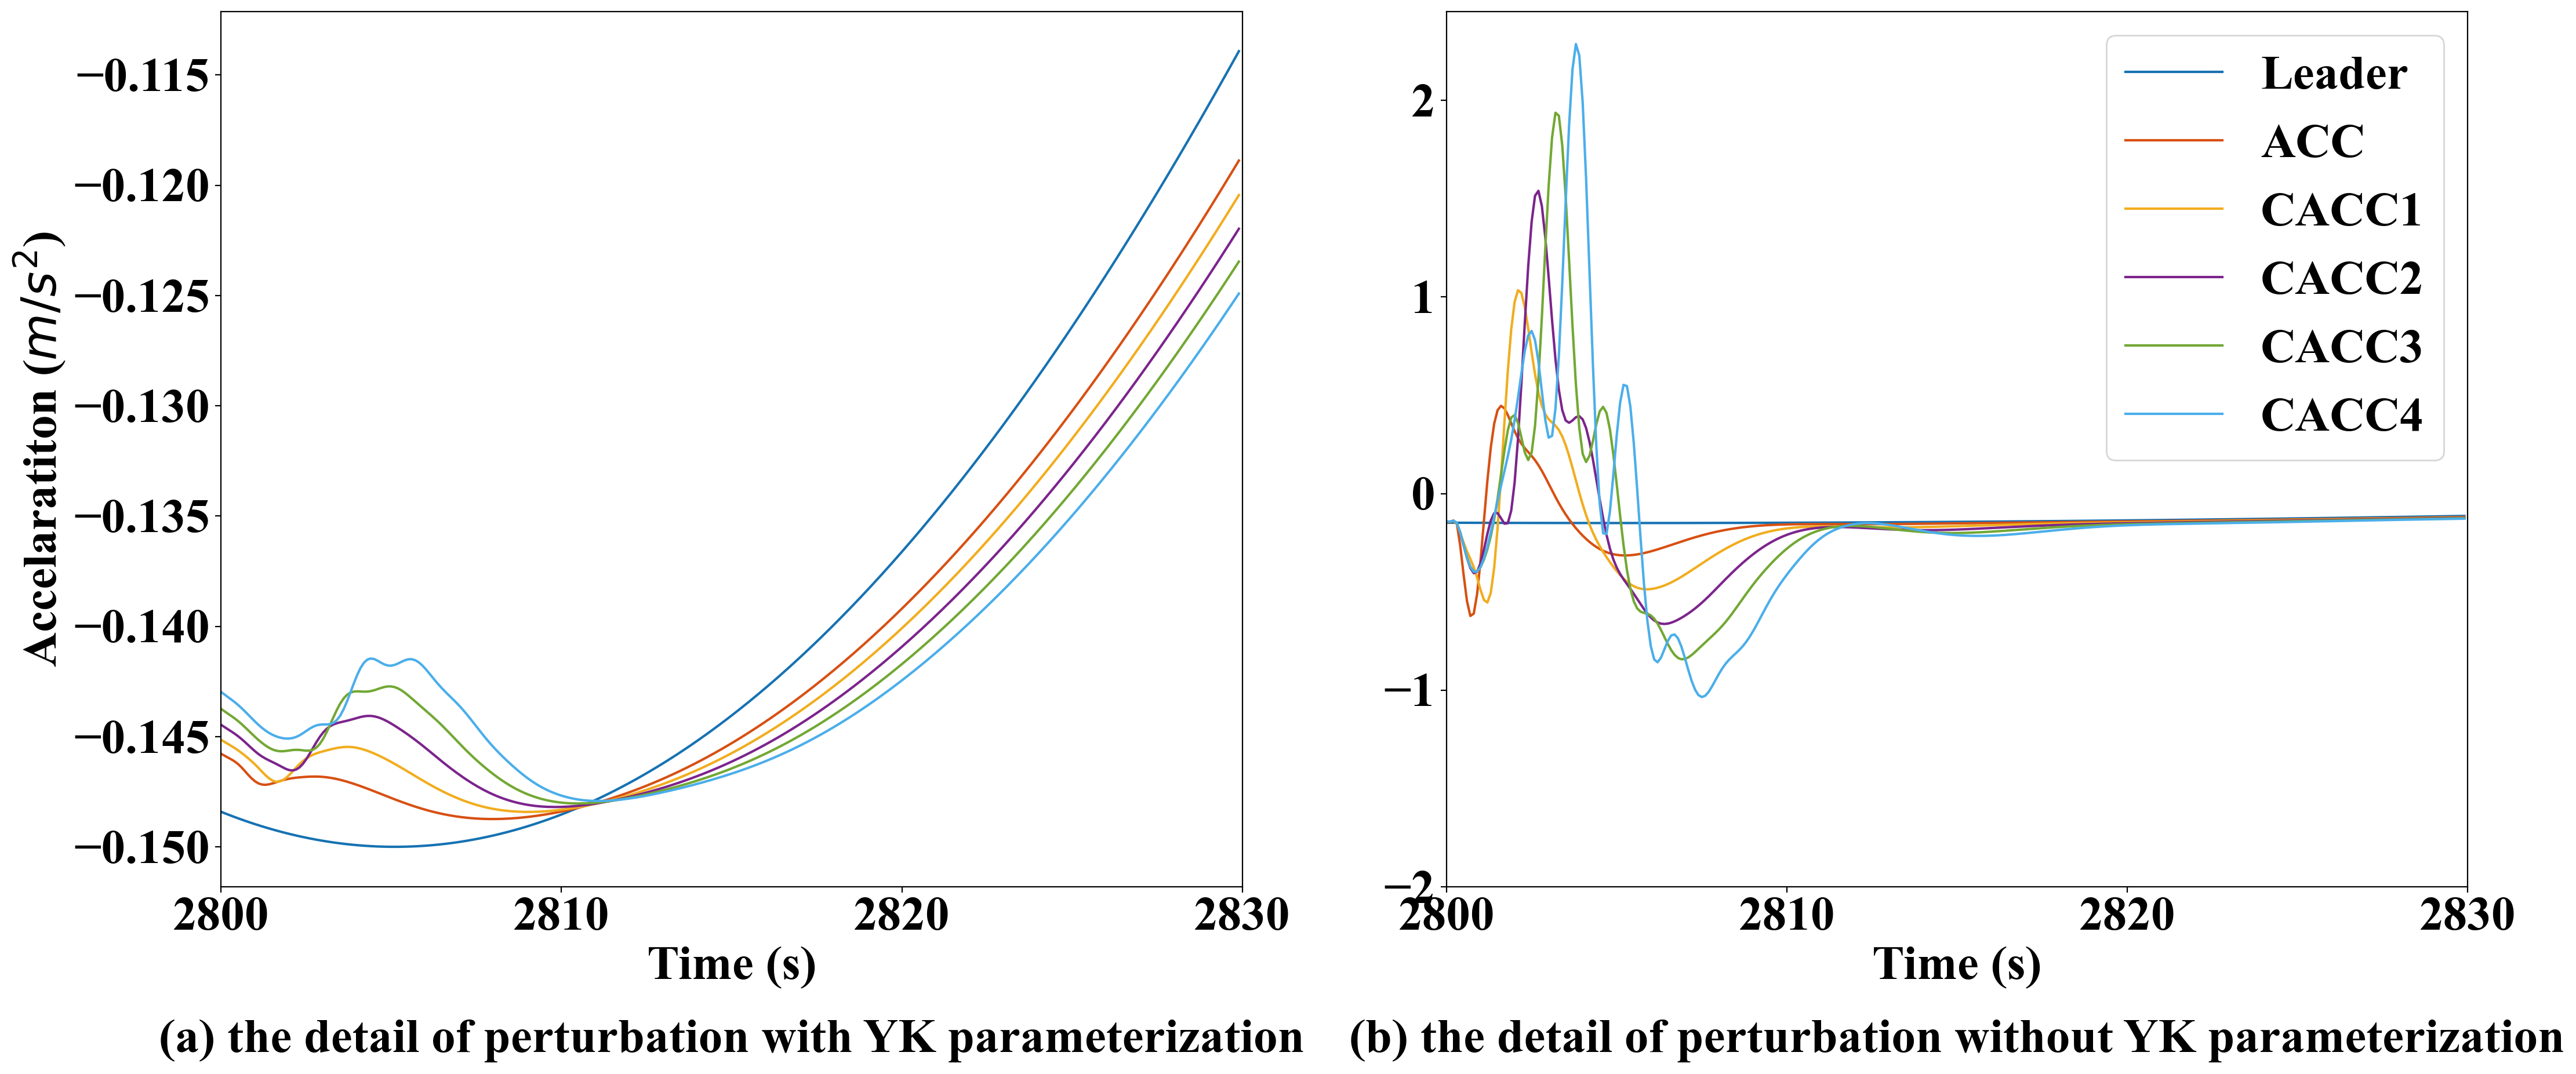
\includegraphics[width=14cm]{figs/extendfig6.png}
% 	\caption{~Detailed perturbation simulation results of experiments five and six: CACPC with or without YK parameterization.}
% 	\label{extend6}
% \end{figure}

\textit{Simulation results}. Fig.~\ref{new5}, \ref{new6} show the results of experiments \uppercase\expandafter{\romannumeral5} and \uppercase\expandafter{\romannumeral6} from global and local perspectives, respectively. The formats of Fig.~\ref{new5}, \ref{new6} are same as Fig.~\ref{new1}, \ref{new2}. For the sake of simplicity, the detailed introduction is omitted. In Fig.~\ref{new5}, the top graph plots the vehicles' accelerations, the median graph plots the vehicles' velocities during the simulation, and the bottom graph plots the time gap during the simulation in each figure.

From Fig.~\ref{new5}, the simulation results under the traffic oscillation scenario are similar to the results with constant velocity. The corresponding detailed simulation results are shown in Fig.~\ref{new6}. The spontaneous perturbations caused by the controller switching are not significant and have the magnitude of 0.015 $m/s^2$ with the YK parameterization, while the perturbation has the magnitude of 2.15$m/s^2$ for the case without YK parameterization under the traffic oscillation scenario. Moreover, a noticeable rise appears in the acceleration subplots, which significantly negatively impacts traffic safety. A conclusion can be drawn that adopting YK parameterization can ensure the smooth switching of the controllers while not adopting it does not, whether it is traffic oscillation or equilibrium state.

\subsubsection{Simulation experiments maintain a constant speed during the multiple CACCs forming processes}
\label{Section 5.2.3}
~\\

\textit{Simulation scenario:} The simulation scenario of experiment \uppercase\expandafter{\romannumeral7} is set as follows: at first, a leader vehicle drives on an infinitely long road under a given speed and acceleration configuration, which is similar to experiment \uppercase\expandafter{\romannumeral1} in Section.~\ref{Section 5.2.1}. There are only three perturbations at the simulation time of 300s, 1000s, and 1700s. Moreover, the forming process of the CACC platoon is that two CACCs join the ACC platoon at the same time, and the forming process repeats twice at the simulation time of 700s and 1400s. Notice that only the case with YK parameterization applied is simulated here because simulation results of the case without YK parameterization are similar to experiment \uppercase\expandafter{\romannumeral2} in Section.~\ref{Section 5.2.1}.

\begin{figure}[htb]
  \centering
  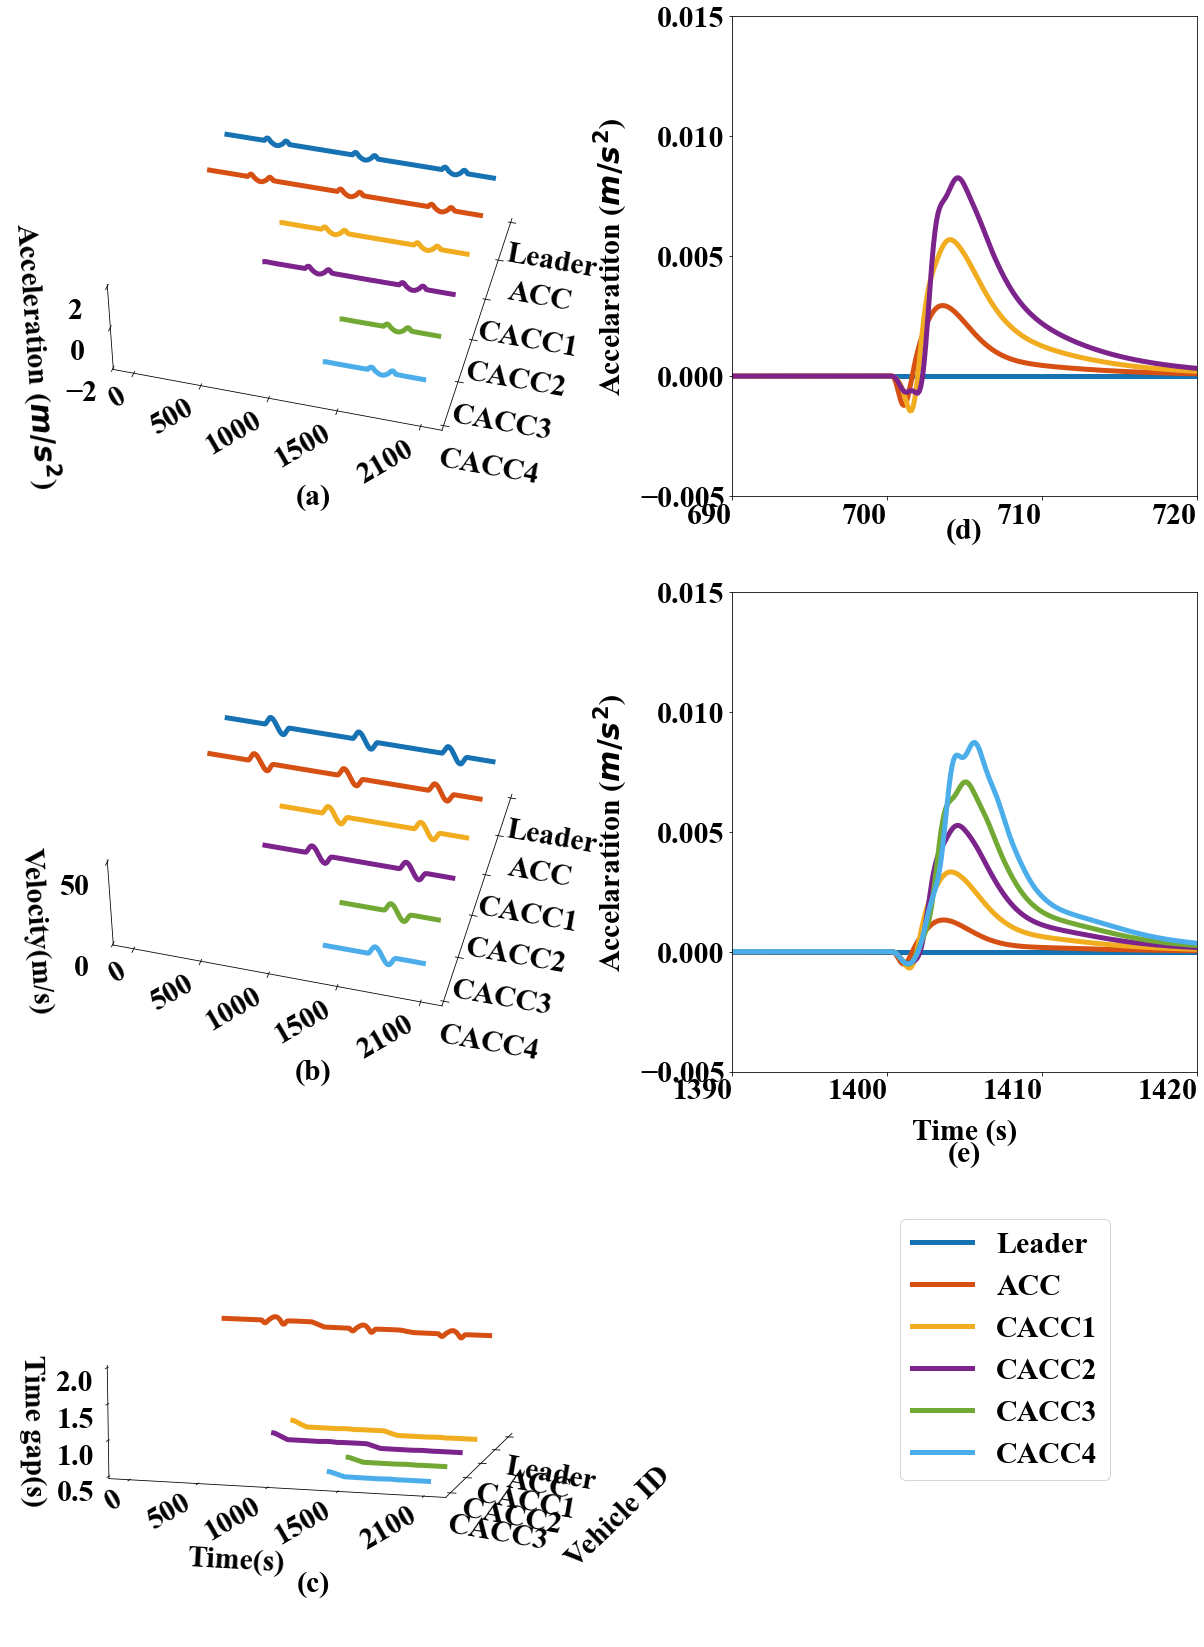
\includegraphics[width=8.5cm]{figs/extendfig7.png}
  \caption{~Simulation results of experiment \uppercase\expandafter{\romannumeral7}: CACPC with YK parameterization under multiple CACCs forming at the same time. (a) Acceleration of simulation results; (b) Velocity of simulation results; (c) Time gap of simulation results; (d) Detailed acceleration of simulation results in 690-720s; (e) Detailed acceleration of simulation results in 1390-1420s}
  \label{extend7}
\end{figure}

\textit{Simulation results}. Fig.~\ref{extend7} shows the results of experiment \uppercase\expandafter{\romannumeral7}. In the left subplot, the top graph plots the vehicles' accelerations, the median graph plots the vehicles' velocities during the simulation, and the bottom graph plots the time gap during the simulation. Moreover, the right subplot shows the detailed acceleration in 690-720s and 1390-1420s to explore the spontaneous perturbation during controllers switching.

Form Fig.~\ref{extend7}, the first conclusion can be drawn that YK parameterization can keep string stability even during the multiple CACCs forming process. The second conclusion can be found in Fig.~\ref{extend7} (d) and (e) that the spontaneous perturbation caused by controllers switching is amplified with multiple CACCs forming. However, the magnitude of the first switching perturbation is still only 0.015 $m/s^2$, which is significantly lower than the case without YK parameterization.






% \subsection{Simulation experiments of the capacity}
% \label{Section 5.3}

% There is no doubt that the most effective and intuitive indicator for evaluating traffic flow is capacity. Therefore, the trends of traffic capacity with and without CACPC are compared through simulation experiments. In addition, CACC MPR is also considered in simulation experiments because CAV-MV heterogeneous traffic flow will continue to exist for a long time. The simulation results are shown in Fig.~\ref{fig13}.

% \begin{figure}
% 	\centering
% 		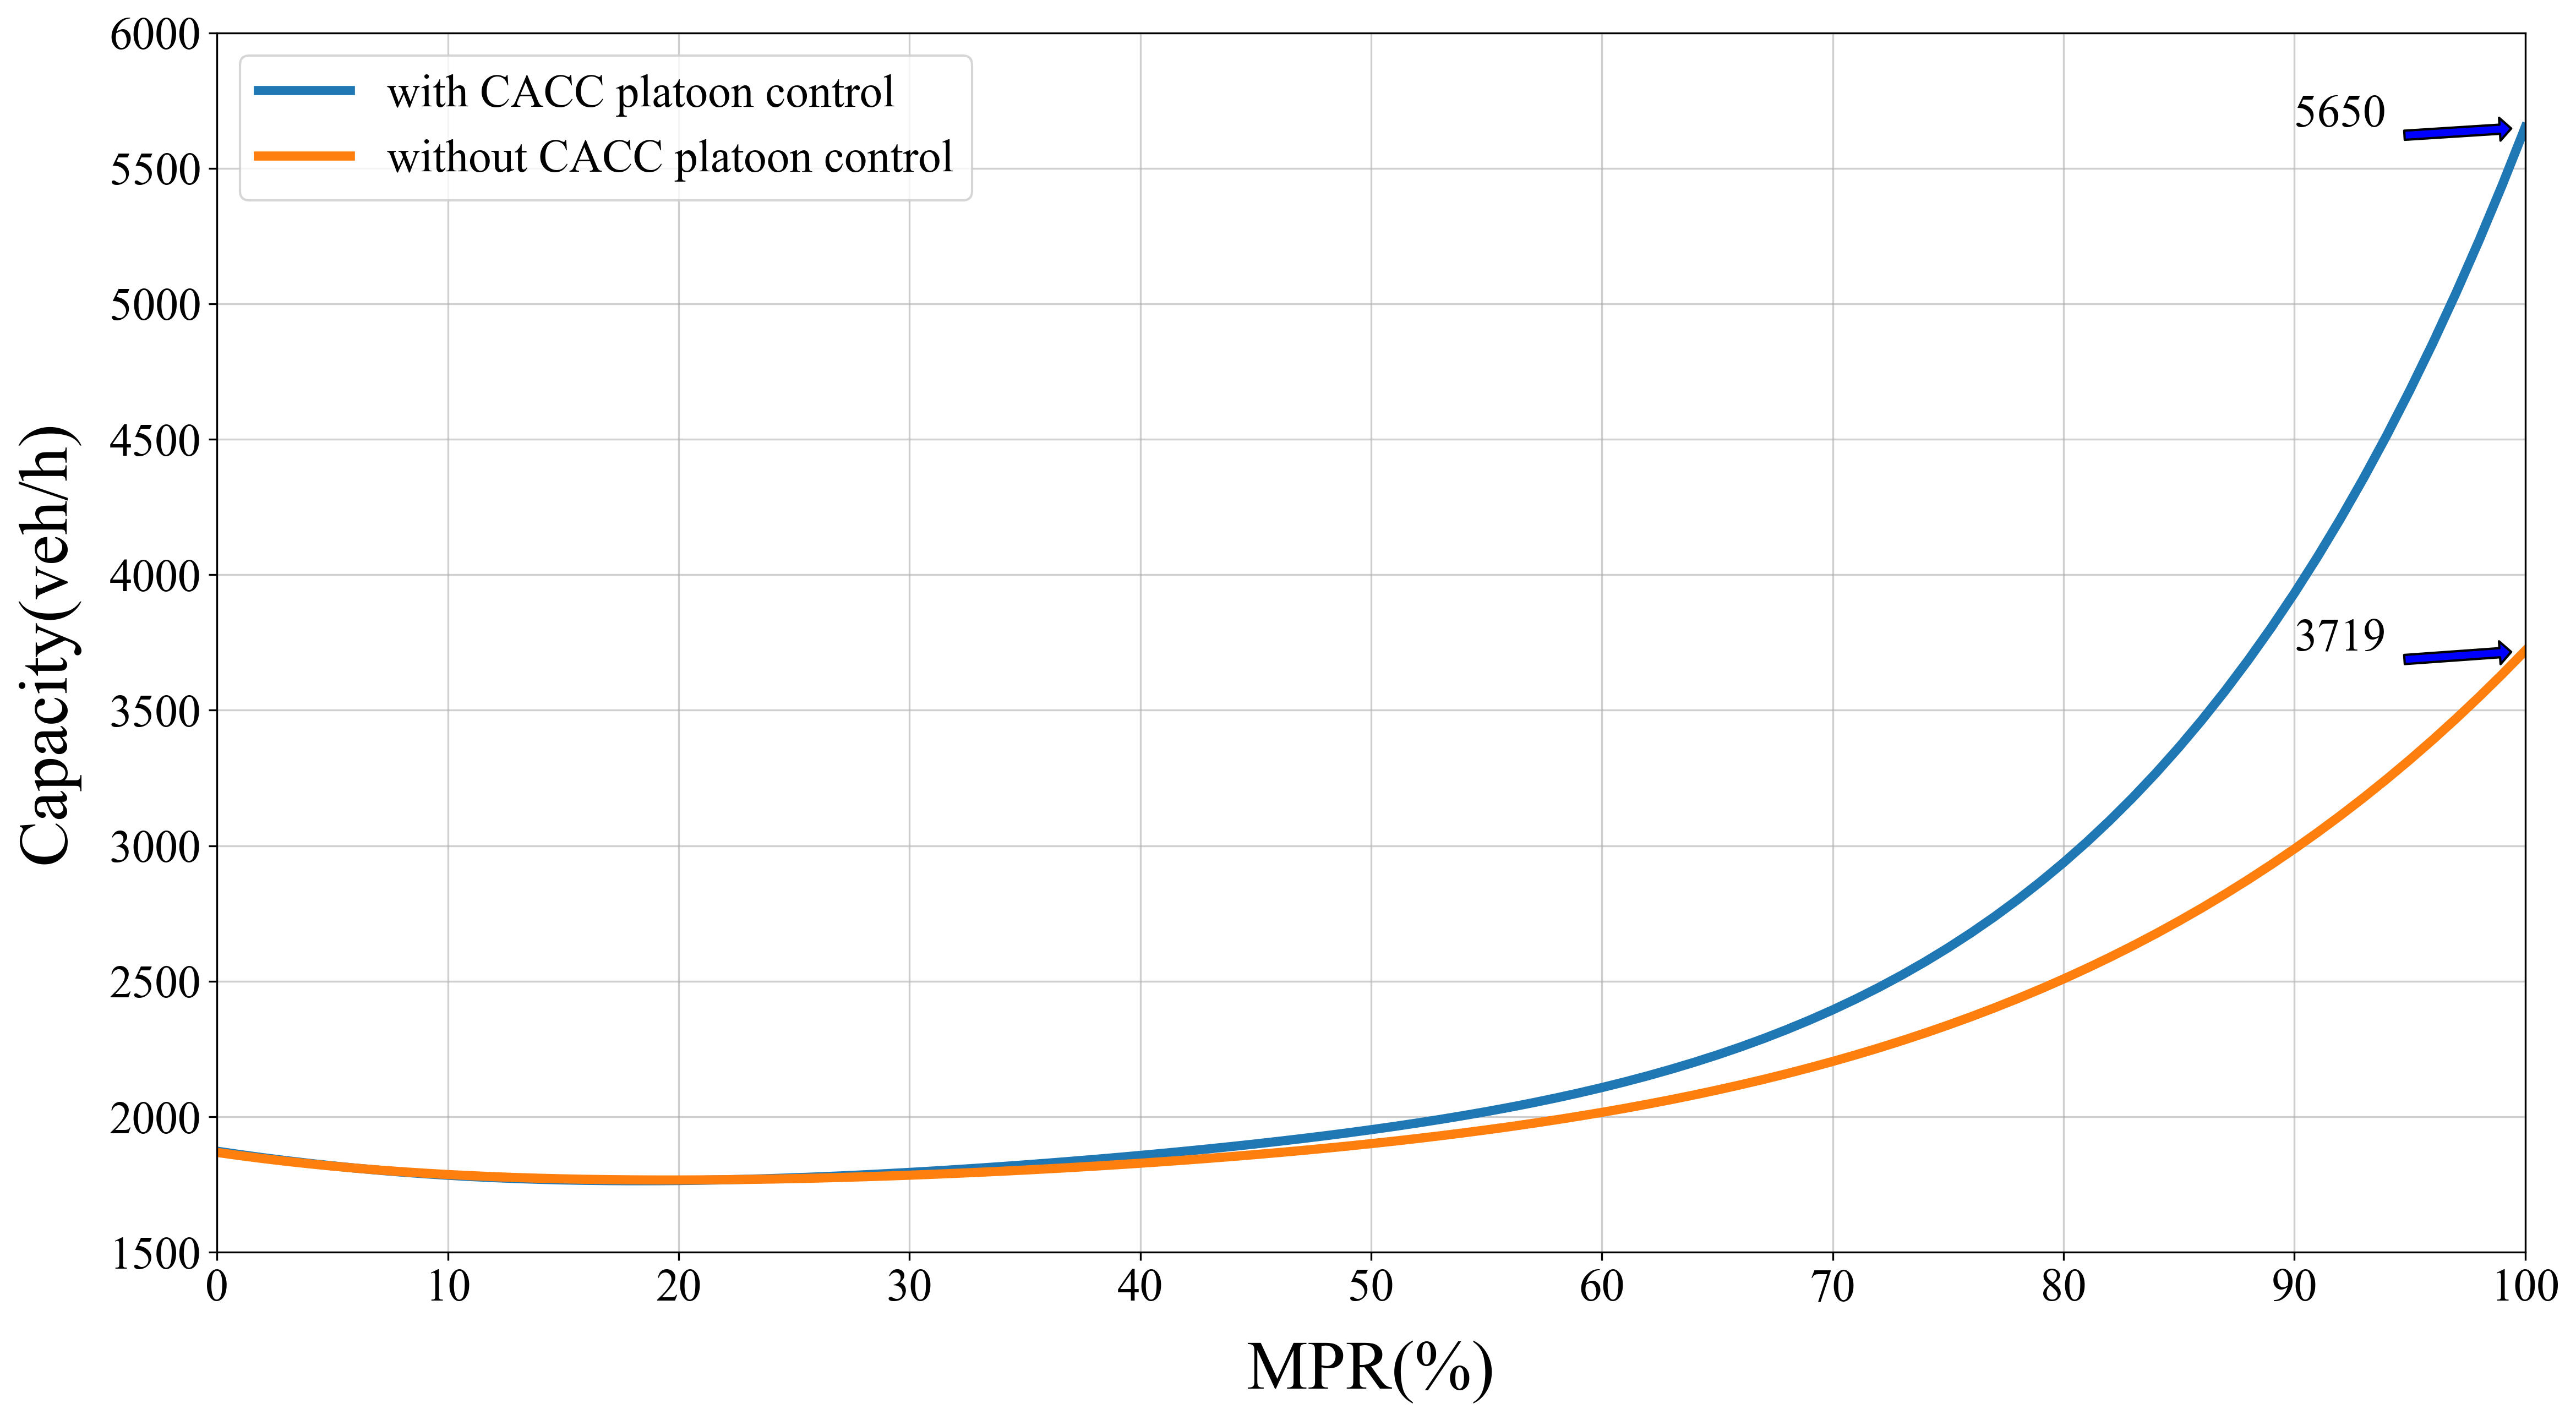
\includegraphics[width=14cm]{figs/fig13.png}
% 	\caption{~Simulation results of the capacity with or without CACPC under different MPR.}
% 	\label{fig13}
% \end{figure}

% A conclusion can be drawn from Fig.~\ref{fig13} that the capacity first increases and then decreases with CAV MPR increasing. It can be found that it will no longer keep the same capacity as the pure MV scenario when the MPR reaches 42\%. When we pay attention to the benefit of CAV involvement on the capacity, we find that as the MPR increases, the capacity gain becomes more obvious, and when the MPR reaches 100\%, the capacity can reach 5650 veh/h, which is 3.02 times that of the pure MV scenario. Moreover, the use of CACPC can improve capacity, and the capacity gain of CACPC will gradually become more significant as the MPR increases since the platoon is more likely to form in the case of high MPR. When the MPR is 100\%, the capacity with CACPC can reach 1.52 times that of the situation without it. From the above analyses, we can conclude that the adoption of CACPC can significantly benefit the traffic capacity, especially under high MPR.

\section{Conclusion}
\label{Section 6}

This paper proposes a switching control model called CACPC to improve the capability by treating the entire CACC platoon as the control object instead of a single vehicle and switching the control as the platoon size changes. In this control model, the string stability of the CACC platoon is analyzed to obtain the margin time gap for different platoon sizes. Then the YK parameterization is applied to ensure the string stability of the CACC platoon when switching between different control modes, and the corresponding tuning function is proposed so that the application of this control mode is not limited by the fixed platoon size. In addition, the effect of YK parameterization on the dynamic performance of CACPC is explored. The following conclusions can be drawn from this paper:
\begin{enumerate}
  \item A new switching control mode for the CACC platoon is proposed capable of adaptively controlling the CACC platoon with different platoon sizes.
  \item CACPC consists of two sets of CACC controllers. YK parameterization ensures stable coupling of the two sets of controllers before and after controller switching to guarantee smooth switching and string stability at different platoon sizes.
  \item The specific process of CACPC control design is given and the corresponding CACPC controller design is carried out.
  \item Combination of tuning function $\gamma$ under different platoon sizes is derived by ensuring that the application range of CACPC is not limited by platoon size.
  \item Adopting YK parameterization can significantly suppress the spontaneous perturbation from 2$m/s^2$ to 0.011$m/s^2$ caused by the controller switch.
  \item YK parameterization can ensure smooth controller switching under the equilibrium state, traffic oscillation, and multiple CACCs forming.
\end{enumerate}





\appendices
\section*{Appendix A. System identification of lower level controller based on field experiments}
\label{AppendixA}

\textit{Experiment preparation}: The experiment was conducted at the Closed test site of National Smart CAV \& C-ITS (Beijing + Hebei) Demonstration Zone Shunyi Base on March 29, 2021. Two cycabs were used for the experiment: autonomous driving vehicles developed by the iDriverplus technology company. The scheme of LiDAR+ millimeter wave + Ultrasonic radar + GPS inertial navigation was adopted as the navigation system, and the distance measurement accuracy is 0.05m. The decision frequency is 20 Hz which equals a 50ms decision interval. Fig.~\ref{experiment} shows the scene of the field experiment.

\begin{figure}
  \centering
  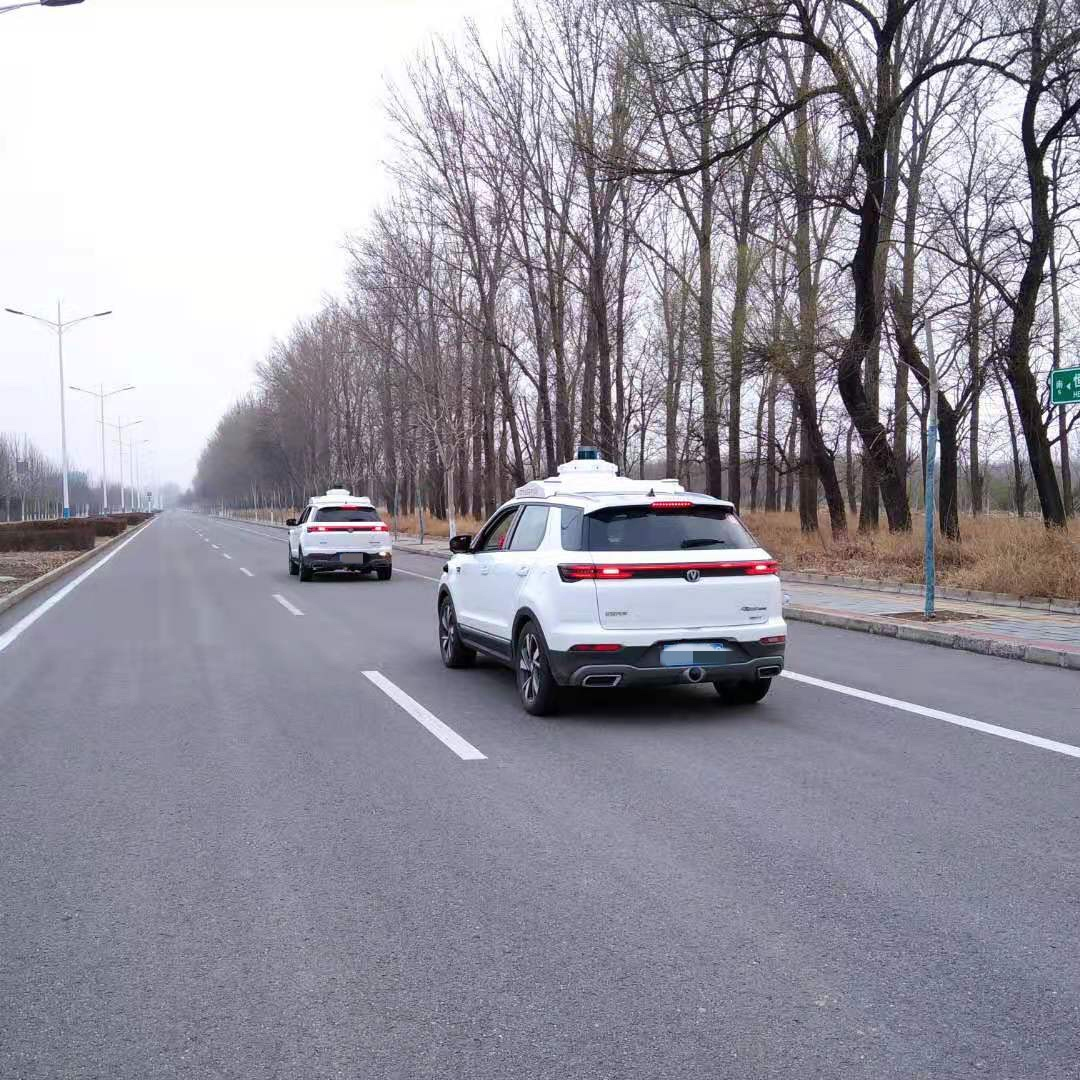
\includegraphics[width=8.5cm]{figs/experiment.jpg}
  \caption{~Field experiment scene.}
  \label{experiment}
\end{figure}

\textit{Experiment scheme}: The experiments were divided into 5 groups. Each group had several rounds, which amounted to a total of 21 rounds of experiments. In each round, the front car drove in accordance with the speed configuration, while the back car used the longitudinal control of the ACC system to follow the front car and record the actual acceleration of the back car. Different groups used different control parameters of the ACC system to ensure that a general conclusion could be drawn.

The control parameters of the ACC system in different experimental groups are shown in communication, and the specific parameter setting is shown in Table.~\ref{table 2}.
\begin{table}
  \caption{~Parameters chosen for different experiment groups.}
  \begin{tabular}{ccccc}
    \hline Index of experiments group & $k_{p}$               & $k_{d}$              & $h_{i}$           & round \\
    \hline $1^{\text {st }}$          & $0.7 \mathrm{s}^{-2}$ & $0  \mathrm{s}^{-1}$ & $2 \mathrm{~s}$   & 2     \\
    \hline $2^{\text {nd }}$          & $0.5 \mathrm{s}^{-2}$ & $0  \mathrm{s}^{-1}$ & $1.8 \mathrm{~s}$ & 5     \\
    \hline $3^{\text {rd }}$          & $0.6 \mathrm{s}^{-2}$ & $0  \mathrm{s}^{-1}$ & $2 \mathrm{~s}$   & 7     \\
    \hline $4^{\text {th }}$          & $0.7 \mathrm{s}^{-2}$ & $0  \mathrm{s}^{-1}$ & $2 \mathrm{~s}$   & 4     \\
    \hline $5^{\text {th }}$          & $0.4 \mathrm{s}^{-2}$ & $0  \mathrm{s}^{-1}$ & $2 \mathrm{~s}$   & 3     \\
    \hline
  \end{tabular}
  \label{table 2}
\end{table}

The experiment data of command acceleration and actual acceleration in the first round are shown in Fig.~\ref{fig14}, where $a_{cmd}$ means the command acceleration and $a_{actual}$ means the actual acceleration.

\begin{figure}
  \centering
  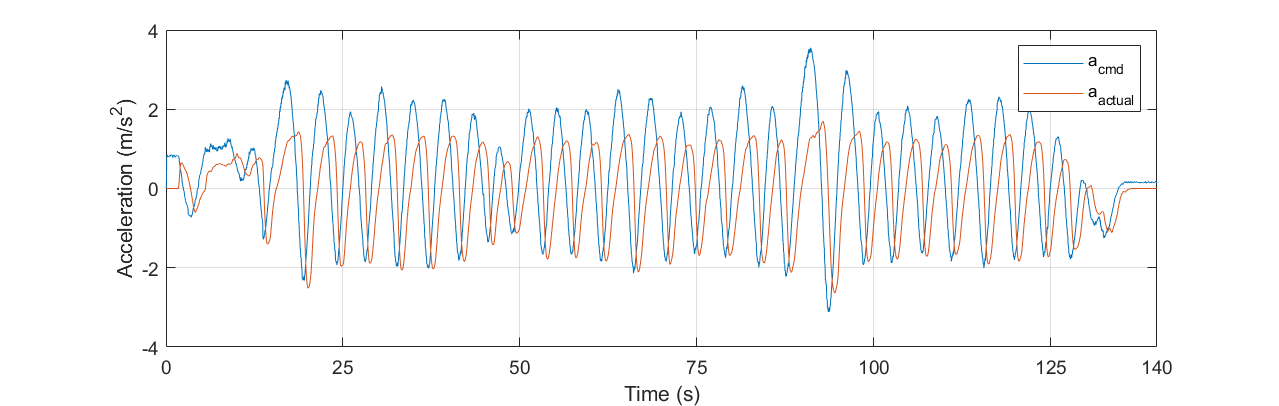
\includegraphics[width=8.5cm]{figs/fig14.png}
  \caption{~Experiment data of the command acceleration and the actual acceleration in first round, where $a_{cmd}$ means the command acceleration and $a_{actual}$ means the actual acceleration.}
  \label{fig14}
\end{figure}

In order to calibrate the transfer function of the lower controller $G_i (s)$, the command acceleration and actual acceleration of the back car in each round are regarded as input and output respectively. Notice that since the output of the lower controller $G_i (s)$ in Fig.~\ref{fig2} is position instead of acceleration, additional second-order integration is applied. Using the System Identification toolbox in MATLAB and setting the desired system type, the transfer function is fitted as follows:
\begin{equation}
  G_{i}(s)=\frac{k_{G}}{s^{2}\left(\tau_{i} s+1\right)} e^{-\phi_{i} s}=\frac{0.9403}{s^{2}(0.7862 s+1)} e^{-0.2 s},
\end{equation}
which keeps fit error to minimun: FPE=0.08699 and MSE=0.0868.

\section*{Appendix B. Proof of the Equation (\ref{Eq17}-\ref{Eq18})}
\label{AppendixB}

The Equation (\ref{Eq17}-\ref{Eq18}) must satisfy the following identities:

\begin{enumerate}
  \item $G=N M^{-1}=\tilde{M}^{-1} \tilde{N}$,
  \item $K_{i}=U_{i} V_{i}^{-1}=\tilde{V}_{i}^{-1} \tilde{U}_{i}$,
  \item    $ \left[\begin{array}{cc}
              \tilde{V}_{i} & -\tilde{U}_{i} \\
              -\tilde{N}    & \tilde{M}
            \end{array}\right]\left[\begin{array}{cc}
              M & U_{i} \\
              N & V_{i}
            \end{array}\right]\\
          =\left[\begin{array}{cc}
              M & U_{i} \\
              N & V_{i}
            \end{array}\right]\left[\begin{array}{cc}
              \tilde{V}_{i} & -\tilde{U}_{i} \\
              -\tilde{N}    & \tilde{M}
            \end{array}\right]\\
          =\left[\begin{array}{cc}
              I & 0 \\
              0 & I
            \end{array}\right].$
\end{enumerate}


\textbf{Proof.} Proof of (a) $G=\tilde{M}^{-1} \tilde{N}$:

\begin{equation}
  \begin{aligned}
     & \tilde{M}^{-1} \tilde{N}                                                                      \\
     & =\left[\begin{array}{cc|c}
        A+B D_{i}^{c} C & B    C_{i}^{c} & B    D_{i}^{c} \\
        B_{i}^{c}   C   & A_{i}^{c}      & B_{i}^{c}      \\
        \hline   C      & -F_{i}^{c}     & I              \\
      \end{array}\right]^{-1} \left[\begin{array}{cc|c}
        A+B    D_{i}^{c} C & B    C_{i}^{c} & B \\
        B_{i}^{c}   C      & A_{i}^{c}      & 0 \\
        \hline    C        & -F_{i}^{c}     & 0 \\
      \end{array}\right] \\
     & =\left[\begin{array}{cc|c}
        A          & B    (C_{i}^{c}+D_{i}^{c}F_{i}^{c}) & -B    D_{i}^{c} \\
        0          & A_{i}^{c}+B_{i}^{c}  F_{i}^{c}      & -B_{i}^{c}      \\
        \hline   C & -F_{i}^{c}                          & I               \\
      \end{array}\right]  \left[\begin{array}{cc|c}
        A+B    D_{i}^{c} C & B    C_{i}^{c} & B \\
        B_{i}^{c}   C      & A_{i}^{c}      & 0 \\
        \hline    C        & -F_{i}^{c}     & 0 \\
      \end{array}\right]     \\
    % 开始写两矩阵相乘
     & =\left[\begin{array}{cccc|c}
        A          & B    (C_{i}^{c}+D_{i}^{c}F_{i}^{c}) & -B    D_{i}^{c}C   & B    D_{i}^{c}F_{i}^{c} & 0 \\
        0          & A_{i}^{c}+B_{i}^{c}   F_{i}^{c}     & -B_{i}^{c}  C      & B_{i}^{c}  F_{i}^{c}    & 0 \\
        0          & 0                                   & A+B    D_{i}^{c} C & B    C_{i}^{c}          & B \\
        0          & 0                                   & B_{i}^{c}   C      & A_{i}^{c}               & 0 \\
        \hline   C & -F_{i}^{c}                          & C                  & -F_{i}^{c}              & 0 \\
      \end{array}\right]                                                  \\
     & =\left[\begin{array}{cccc|c}
        A          & B    (C_{i}^{c}+D_{i}^{c}F_{i}^{c}) & 0                  & 0           & B \\
        0          & A_{i}^{c}+B_{i}^{c} F_{i}^{c}       & 0                  & 0           & 0 \\
        0          & 0                                   & A+B    D_{i}^{c} C & B C_{i}^{c} & B \\
        0          & 0                                   & B_{i}^{c}   C      & A_{i}^{c}   & 0 \\
        \hline   C & -F_{i}^{c}                          & 0                  & 0           & 0 \\
      \end{array}\right]                                                 \\
    % 补充矩阵讲解推导公式
     & =\left[\begin{array}{c|c}
        A        & B \\
        \hline C & 0 \\
      \end{array}\right] ,
  \end{aligned}
  % \label{Eq18}
\end{equation}
where $\mathbf{T}=\left[\begin{array}{cccc}\mathbf{I} & 0 & -\mathbf{I} & 0 \\ 0 & \mathbf{I} & 0 & -\mathbf{I} \\ 0 & 0 & \mathbf{I} & 0 \\ 0 & 0 & 0 & \mathbf{I}\end{array}\right], \quad \mathbf{T}^{-1}=\left[\begin{array}{cccc}\mathbf{I} & 0 & \mathbf{I} & 0 \\ 0 & \mathbf{I} & 0 & \mathbf{I} \\ 0 & 0 & \mathbf{I} & 0 \\ 0 & 0 & 0 & \mathbf{I}\end{array}\right]$  is adopted in the similarity transformation.
The proofs that $G=N M^{-1}$ and (ii) are analogous.

\textbf{Proof.} Proof of (c) $\left[\begin{array}{cc}
      M & U_{i} \\
      N & V_{i}
    \end{array}\right]\left[\begin{array}{cc}
      \tilde{V}_{i} & -\tilde{U}_{i} \\
      -\tilde{N}    & \tilde{M}
    \end{array}\right]=\left[\begin{array}{cc}
      I & 0 \\
      0 & I
    \end{array}\right].$

\begin{equation}
  \begin{aligned}
     & \left[\begin{array}{cc}
        M & U_{i} \\
        N & V_{i}
      \end{array}\right]^{-1}  \\
     & =\left[\begin{array}{cc|cc}
        A+B F     & 0                             & -B & 0         \\
        0         & A_{i}^{c}+B_{i}^{c} F_{i}^{c} & 0  & B_{i}^{c} \\
        \hline -F & C_{i}^{c}+D_{i}^{c} F_{i}^{c} & I  & D_{i}^{c} \\
        -C        & F_{i}^{c}                     & 0  & I
      \end{array}\right]^{-1} \\
     & =\left[\begin{array}{cc|cc}
        A+B  D_{i}^{c} C          & B  C_{i}^{c} & -B & B  D_{i}^{c} \\
        B_{i}^{c} C               & A_{i}^{c}    & 0  & B_{i}^{c}    \\
        \hline F_{i}- D_{i}^{c} C & -C_{i}^{c}   & I  & -D_{i}^{c}   \\
        C                         & -F_{i}^{c}   & 0  & I            \\
      \end{array}\right]      \\
     & =\left[\begin{array}{cc}
        \tilde{V}_{i} & -\tilde{U}_{i} \\
        -\tilde{N}    & \tilde{M}
      \end{array}\right].
  \end{aligned}
\end{equation}

\textbf{Q.E.D.}

% if have a single appendix:
%\appendix[Proof of the Zonklar Equations]
% or
%\appendix % for no appendix heading
% do not use \section anymore after \appendix, only \section*
% is possibly needed

% use appendices with more than one appendix
% then use \section to start each appendix
% you must declare a \section before using any
% \subsection or using \label (\appendices by itself
% starts a section numbered zero.)
%


% \appendices
% \section{Proof of the First Zonklar Equation}
% Appendix one text goes here.

% you can choose not to have a title for an appendix
% if you want by leaving the argument blank
% \section{}
% Appendix two text goes here.


% use section* for acknowledgment
\section*{Acknowledgment}


This research was sponsored by National Science Foundation of China (No. 51878161, No. 71931002, No.72288101 and No.52072067).


% Can use something like this to put references on a page
% by themselves when using endfloat and the captionsoff option.
\ifCLASSOPTIONcaptionsoff
  \newpage
\fi



% trigger a \newpage just before the given reference
% number - used to balance the columns on the last page
% adjust value as needed - may need to be readjusted if
% the document is modified later
%\IEEEtriggeratref{8}
% The "triggered" command can be changed if desired:
%\IEEEtriggercmd{\enlargethispage{-5in}}

% references section
% can use a bibliography generated by BibTeX as a .bbl file
% BibTeX documentation can be easily obtained at:
% http://mirror.ctan.org/biblio/bibtex/contrib/doc/
% The IEEEtran BibTeX style support page is at:
% http://www.michaelshell.org/tex/ieeetran/bibtex/
\bibliographystyle{IEEEtran}
% argument is your BibTeX string definitions and bibliography database(s)
%\bibliography{IEEEabrv,../bib/paper}
%\bibliography{cas-refs}
% <OR> manually copy in the resultant .bbl file
% set second argument of \begin to the number of references
% (used to reserve space for the reference number labels box)

\bibliography{cas-refs}
% \begin{thebibliography}{34}
% \providecommand{\natexlab}[1]{#1}
% \providecommand{\url}[1]{\texttt{#1}}
% \expandafter\ifx\csname urlstyle\endcsname\relax
%   \providecommand{\doi}[1]{doi: #1}\else
%   \providecommand{\doi}{doi: \begingroup \urlstyle{rm}\Url}\fi

% \bibitem[Wang et~al.(2019)Wang, Bian, Shladover, Wu, Li, and
%   Barth]{wang2019survey}
% Ziran Wang, Yougang Bian, Steven~E Shladover, Guoyuan Wu, Shengbo~Eben Li, and
%   Matthew~J Barth.
% \newblock A survey on cooperative longitudinal motion control of multiple
%   connected and automated vehicles.
% \newblock \emph{IEEE Intelligent Transportation Systems Magazine}, 12\penalty0
%   (1):\penalty0 4--24, 2019.

% \bibitem[Shladover et~al.(2015)Shladover, Nowakowski, Lu, and
%   Ferlis]{shladover2015cooperative}
% Steven~E Shladover, Christopher Nowakowski, Xiao-Yun Lu, and Robert Ferlis.
% \newblock Cooperative adaptive cruise control: Definitions and operating
%   concepts.
% \newblock \emph{Transportation Research Record}, 2489\penalty0 (1):\penalty0
%   145--152, 2015.

% \bibitem[Wang et~al.(2020{\natexlab{b}})Wang, Zheng, Xu, Wang, and
%   Li]{wang2020controllability}
% Jiawei Wang, Yang Zheng, Qing Xu, Jianqiang Wang, and Keqiang Li.
% \newblock Controllability analysis and optimal control of mixed traffic flow
%   with human-driven and autonomous vehicles.
% \newblock \emph{IEEE Transactions on Intelligent Transportation Systems},
%   2020{\natexlab{b}}.

% \bibitem[Hall and Chin(2005)]{hall2005vehicle}
% Randolph Hall and Chinan Chin.
% \newblock Vehicle sorting for platoon formation: Impacts on highway entry and
%   throughput.
% \newblock \emph{Transportation Research Part C: Emerging Technologies},
%   13\penalty0 (5-6):\penalty0 405--420, 2005.


% \bibitem[Yanyan~Qin(2021)]{qin2021LWR}
% Daiheng~Ni Yanyan~Qin, Hao~Wang.
% \newblock Lwr model for traffic flow mixed with cacc vehicles.
% \newblock \emph{Transportation Science}, 2021.


% \bibitem[Zhang et~al.(2020)Zhang, Bai, Hu, and Wang]{zhang2020control}
% Yu~Zhang, Yu~Bai, Jia Hu, and Meng Wang.
% \newblock Control design, stability analysis, and traffic flow implications for
%   cooperative adaptive cruise control systems with compensation of
%   communication delay.
% \newblock \emph{Transportation Research Record}, 2674\penalty0 (8):\penalty0
%   638--652, 2020.


% \bibitem[Navas and Milan{\'e}s(2019)]{navas2019mixing}
% Francisco Navas and Vicente Milan{\'e}s.
% \newblock Mixing v2v-and non-v2v-equipped vehicles in car following.
% \newblock \emph{Transportation research part C: emerging technologies},
%   108:\penalty0 167--181, 2019.

% \bibitem[Wang et~al.(2020{\natexlab{a}})Wang, Gong, Zhou, Li, and
%   Peeta]{wang2020cooperative}
% Chaojie Wang, Siyuan Gong, Anye Zhou, Tao Li, and Srinivas Peeta.
% \newblock Cooperative adaptive cruise control for connected autonomous vehicles
%   by factoring communication-related constraints.
% \newblock \emph{Transportation Research Part C: Emerging Technologies},
%   113:\penalty0 124--145, 2020{\natexlab{a}}.

% \bibitem[Li et~al.(2020)Li, Bian, Li, Xu, and Wang]{li2020distributed}
% Keqiang Li, Yougang Bian, Shengbo~Eben Li, Biao Xu, and Jianqiang Wang.
% \newblock Distributed model predictive control of multi-vehicle systems with
%   switching communication topologies.
% \newblock \emph{Transportation Research Part C: Emerging Technologies},
%   118:\penalty0 102717, 2020.

% \bibitem[Zhou et~al.(2020)Zhou, Gong, Wang, and Peeta]{zhou2020smooth}
% Anye Zhou, Siyuan Gong, Chaojie Wang, and Srinivas Peeta.
% \newblock Smooth-switching control-based cooperative adaptive cruise control by
%   considering dynamic information flow topology.
% \newblock \emph{Transportation Research Record}, 2674\penalty0 (4):\penalty0
%   444--458, 2020.

% \bibitem[Zheng et~al.(2015)Zheng, Li, Wang, Cao, and Li]{zheng2015stability}
% Yang Zheng, Shengbo~Eben Li, Jianqiang Wang, Dongpu Cao, and Keqiang Li.
% \newblock Stability and scalability of homogeneous vehicular platoon: Study on
%   the influence of information flow topologies.
% \newblock \emph{IEEE Transactions on intelligent transportation systems},
%   17\penalty0 (1):\penalty0 14--26, 2015.

% \bibitem[Jia et~al.(2015)Jia, Lu, Wang, Zhang, and Shen]{jia2015survey}
% Dongyao Jia, Kejie Lu, Jianping Wang, Xiang Zhang, and Xuemin Shen.
% \newblock A survey on platoon-based vehicular cyber-physical systems.
% \newblock \emph{IEEE communications surveys \& tutorials}, 18\penalty0
%   (1):\penalty0 263--284, 2015.

% \bibitem[Ma et~al.(2020)Ma, Wang, Yang, Wu, Zhu, Gelbal, Aksun-Guvenc, and
%   Guvenc]{ma2020stability}
% Fangwu Ma, Jiawei Wang, Yu~Yang, Liang Wu, Sheng Zhu, Sukru~Yaren Gelbal, Bilin
%   Aksun-Guvenc, and Levent Guvenc.
% \newblock Stability design for the homogeneous platoon with communication time
%   delay.
% \newblock \emph{Automotive Innovation}, 3:\penalty0 101--110, 2020.

% \bibitem[Zheng et~al.(2014)Zheng, Li, Wang, Li, et~al.]{zheng2014influence}
% Yang Zheng, Shengbo~Eben Li, Jianqiang Wang, Keqiang Li, et~al.
% \newblock Influence of information flow topology on closed-loop stability of
%   vehicle platoon with rigid formation.
% \newblock In \emph{17th International IEEE Conference on Intelligent
%   Transportation Systems (ITSC)}, pages 2094--2100. IEEE, 2014.

% \bibitem[Farah and Koutsopoulos(2014)]{farah2014cooperative}
% Haneen Farah and Haris~N Koutsopoulos.
% \newblock Do cooperative systems make drivers’ car-following behavior safer?
% \newblock \emph{Transportation research part C: emerging technologies},
%   41:\penalty0 61--72, 2014.

% \bibitem[Yu and Shi(2015)]{yu2015effects}
% Shaowei Yu and Zhongke Shi.
% \newblock The effects of vehicular gap changes with memory on traffic flow in
%   cooperative adaptive cruise control strategy.
% \newblock \emph{Physica A: Statistical Mechanics and its Applications},
%   428:\penalty0 206--223, 2015.

% \bibitem[Li et~al.(2015)Li, Li, Xu, and Qian]{li2015stability}
% Zhipeng Li, Wenzhong Li, Shangzhi Xu, and Yeqing Qian.
% \newblock Stability analysis of an extended intelligent driver model and its
%   simulations under open boundary condition.
% \newblock \emph{Physica A: Statistical Mechanics and its Applications},
%   419:\penalty0 526--536, 2015.

% \bibitem[Fernandes and Nunes(2014)]{fernandes2014multiplatooning}
% Pedro Fernandes and Urbano Nunes.
% \newblock Multiplatooning leaders positioning and cooperative behavior
%   algorithms of communicant automated vehicles for high traffic capacity.
% \newblock \emph{IEEE Transactions on Intelligent Transportation Systems},
%   16\penalty0 (3):\penalty0 1172--1187, 2014.

% \bibitem[Milan{\'e}s and Shladover(2014)]{milanes2014modeling}
% Vicente Milan{\'e}s and Steven~E Shladover.
% \newblock Modeling cooperative and autonomous adaptive cruise control dynamic
%   responses using experimental data.
% \newblock \emph{Transportation Research Part C: Emerging Technologies},
%   48:\penalty0 285--300, 2014.

% \bibitem[Milan{\'e}s et~al.(2013)Milan{\'e}s, Shladover, Spring, Nowakowski,
%   Kawazoe, and Nakamura]{milanes2013cooperative}
% Vicente Milan{\'e}s, Steven~E Shladover, John Spring, Christopher Nowakowski,
%   Hiroshi Kawazoe, and Masahide Nakamura.
% \newblock Cooperative adaptive cruise control in real traffic situations.
% \newblock \emph{IEEE Transactions on intelligent transportation systems},
%   15\penalty0 (1):\penalty0 296--305, 2013.

% \bibitem[Dey et~al.(2015)Dey, Yan, Wang, Wang, Shen, Chowdhury, Yu, Qiu, and
%   Soundararaj]{dey2015review}
% Kakan~C Dey, Li~Yan, Xujie Wang, Yue Wang, Haiying Shen, Mashrur Chowdhury, Lei
%   Yu, Chenxi Qiu, and Vivekgautham Soundararaj.
% \newblock A review of communication, driver characteristics, and controls
%   aspects of cooperative adaptive cruise control (cacc).
% \newblock \emph{IEEE Transactions on Intelligent Transportation Systems},
%   17\penalty0 (2):\penalty0 491--509, 2015.

% \bibitem[Ngoduy(2013)]{ngoduy2013analytical}
% Dong Ngoduy.
% \newblock Analytical studies on the instabilities of heterogeneous intelligent
%   traffic flow.
% \newblock \emph{Communications in Nonlinear Science and Numerical Simulation},
%   18\penalty0 (10):\penalty0 2699--2706, 2013.

% \bibitem[Yao et~al.(2021)Yao, Xu, Jiang, and Hu]{yao2021linear}
% Zhihong Yao, Taorang Xu, Yangsheng Jiang, and Rong Hu.
% \newblock Linear stability analysis of heterogeneous traffic flow considering
%   degradations of connected automated vehicles and reaction time.
% \newblock \emph{Physica A: Statistical Mechanics and its Applications},
%   561:\penalty0 125218, 2021.

% \bibitem[Jin and Orosz(2014)]{jin2014dynamics}
% I~Ge Jin and G{\'a}bor Orosz.
% \newblock Dynamics of connected vehicle systems with delayed acceleration
%   feedback.
% \newblock \emph{Transportation Research Part C: Emerging Technologies},
%   46:\penalty0 46--64, 2014.

% \bibitem[Sun et~al.(2018)Sun, Zheng, and Sun]{sun2018stability}
% Jie Sun, Zuduo Zheng, and Jian Sun.
% \newblock Stability analysis methods and their applicability to car-following
%   models in conventional and connected environments.
% \newblock \emph{Transportation research part B: methodological}, 109:\penalty0
%   212--237, 2018.

% \bibitem[Chang et~al.(2020)Chang, Li, Rong, Zhao, et~al.]{chang2020analysis}
% Xin Chang, Haijian Li, Jian Rong, Xiaohua Zhao, et~al.
% \newblock Analysis on traffic stability and capacity for mixed traffic flow
%   with platoons of intelligent connected vehicles.
% \newblock \emph{Physica A: Statistical Mechanics and its Applications},
%   557:\penalty0 124829, 2020.

% \bibitem[Li et~al.(2017)Li, Wang, Wang, Xing, Liu, and Wei]{li2017evaluation}
% Ye~Li, Hao Wang, Wei Wang, Lu~Xing, Shanwen Liu, and Xueyan Wei.
% \newblock Evaluation of the impacts of cooperative adaptive cruise control on
%   reducing rear-end collision risks on freeways.
% \newblock \emph{Accident Analysis \& Prevention}, 98:\penalty0 87--95, 2017.

% \bibitem[Kesting et~al.(2008)Kesting, Treiber, Sch{\"o}nhof, and
%   Helbing]{kesting2008adaptive}
% Arne Kesting, Martin Treiber, Martin Sch{\"o}nhof, and Dirk Helbing.
% \newblock Adaptive cruise control design for active congestion avoidance.
% \newblock \emph{Transportation Research Part C: Emerging Technologies},
%   16\penalty0 (6):\penalty0 668--683, 2008.

% \bibitem[Kesting et~al.(2007)Kesting, Treiber, Sch{\"o}nhof, Kranke, and
%   Helbing]{kesting2007jam}
% Arne Kesting, Martin Treiber, Martin Sch{\"o}nhof, Florian Kranke, and Dirk
%   Helbing.
% \newblock Jam-avoiding adaptive cruise control (acc) and its impact on traffic
%   dynamics.
% \newblock In \emph{Traffic and Granular Flow’05}, pages 633--643. Springer,
%   2007.

% \bibitem[Hafeez et~al.(2013)Hafeez, Zhao, Ma, and Mark]{hafeez2013performance}
% Khalid~Abdel Hafeez, Lian Zhao, Bobby Ma, and Jon~W Mark.
% \newblock Performance analysis and enhancement of the dsrc for vanet's safety
%   applications.
% \newblock \emph{IEEE Transactions on Vehicular Technology}, 62\penalty0
%   (7):\penalty0 3069--3083, 2013.

% \bibitem[Gong et~al.(2016)Gong, Shen, and Du]{gong2016constrained}
% Siyuan Gong, Jinglai Shen, and Lili Du.
% \newblock Constrained optimization and distributed computation based car
%   following control of a connected and autonomous vehicle platoon.
% \newblock \emph{Transportation Research Part B: Methodological}, 94:\penalty0
%   314--334, 2016.

% \bibitem[Li et~al.(2014)Li, Cui, An, and Parsafard]{li2014stop}
% Xiaopeng Li, Jianxun Cui, Shi An, and Mohsen Parsafard.
% \newblock Stop-and-go traffic analysis: Theoretical properties, environmental
%   impacts and oscillation mitigation.
% \newblock \emph{Transportation Research Part B: Methodological}, 70:\penalty0
%   319--339, 2014.

% \bibitem[Panis et~al.(2006)Panis, Broekx, and Liu]{panis2006modelling}
% Luc~Int Panis, Steven Broekx, and Ronghui Liu.
% \newblock Modelling instantaneous traffic emission and the influence of traffic
%   speed limits.
% \newblock \emph{Science of the total environment}, 371\penalty0 (1-3):\penalty0
%   270--285, 2006.

% \end{thebibliography}


% biography section
% 
% If you have an EPS/PDF photo (graphicx package needed) extra braces are
% needed around the contents of the optional argument to biography to prevent
% the LaTeX parser from getting confused when it sees the complicated
% \includegraphics command within an optional argument. (You could create
% your own custom macro containing the \includegraphics command to make things
% simpler here.)
%\begin{IEEEbiography}[{\includegraphics[width=1in,height=1.25in,clip,keepaspectratio]{mshell}}]{Michael Shell}
% or if you just want to reserve a space for a photo:

% \begin{IEEEbiography}{Michael Shell}
% Biography text here.
% \end{IEEEbiography}

% % if you will not have a photo at all:
% \begin{IEEEbiographynophoto}{John Doe}
% Biography text here.
% \end{IEEEbiographynophoto}

% insert where needed to balance the two columns on the last page with
% biographies
%\newpage

% \begin{IEEEbiographynophoto}{Jane Doe}
% Biography text here.
% \end{IEEEbiographynophoto}

% You can push biographies down or up by placing
% a \vfill before or after them. The appropriate
% use of \vfill depends on what kind of text is
% on the last page and whether or not the columns
% are being equalized.

%\vfill

% Can be used to pull up biographies so that the bottom of the last one
% is flush with the other column.
%\enlargethispage{-5in}



% that's all folks
\end{document}


